\documentclass[11pt,a4paper,oneside]{book}

% Load all styling and custom packages
% Preamble for IITM Financial Forensics (BSMS4003)
% Common Preamble for IITM BS Textbook Project
\usepackage[utf8]{inputenc}
\usepackage[T1]{fontenc}
\usepackage{geometry}
\geometry{
    a4paper,
    left=0.9in,
    right=0.9in,
    top=1.0in,
    bottom=1.0in
}

% Typography
\usepackage{palatino} % Clean serif body font
\usepackage[scaled]{helvet} % Helvetica for sans-serif
\usepackage{microtype} % Better word spacing and justifications

% Math Packages
\usepackage{amsmath}
\usepackage{amssymb}
\usepackage{amsthm}
\usepackage{mathtools}
\usepackage{bm} % Bold math symbols
\usepackage{array}
\usepackage{booktabs}
\usepackage{pgfplots}
\pgfplotsset{compat=1.18}
\IfFileExists{venndiagram.sty}{%
  \usepackage{venndiagram}%
}{%
  \makeatletter
  \newenvironment{venndiagram2sets}[1][]{%
    \begin{tikzpicture}[scale=0.55, transform shape]%
      \draw[thick] (-2,-1.5) rectangle (3.5,1.5);
      \node at (3.1,1.1) {$S$};
      \draw[thick] (0,0) circle (1.2cm);
      \draw[thick] (1.5,0) circle (1.2cm);
      \node at (-0.5,0.7) {$A$};
      \node at (2.0,0.7) {$B$};
      \providecommand{\fillA}{\fill[gray!40,opacity=0.6] (0,0) circle (1.2cm);}%
      \providecommand{\fillB}{\fill[gray!40,opacity=0.6] (1.5,0) circle (1.2cm);}%
      \providecommand{\fillACapB}{%
        \begin{scope}%
          \clip (0,0) circle (1.2cm);%
          \fill[gray!60] (1.5,0) circle (1.2cm);%
        \end{scope}%
      }%
      \providecommand{\fillOnlyA}{%
        \begin{scope}%
          \clip (-2,-1.5) rectangle (3.5,1.5);%
          \fill[gray!40] (0,0) circle (1.2cm);%
          \fill[white] (1.5,0) circle (1.2cm);%
          \draw[thick] (0,0) circle (1.2cm);%
          \draw[thick] (1.5,0) circle (1.2cm);%
        \end{scope}%
      }%
      \providecommand{\fillNotA}{%
        \fill[gray!30] (-2,-1.5) rectangle (3.5,1.5);%
        \fill[white] (0,0) circle (1.2cm);%
        \draw[thick] (0,0) circle (1.2cm);%
        \draw[thick] (1.5,0) circle (1.2cm);%
      }%
  }{%
    \end{tikzpicture}%
  }
  \makeatother
}

% Headings styling
\usepackage{titlesec}
\titleformat{\chapter}[display]
  {\normalfont\sffamily\huge\bfseries\color{primarydark}}
  {\chaptername\ \thechapter}{20pt}{\Huge}
\titleformat{\section}
  {\normalfont\sffamily\Large\bfseries\color{primarydark}}
  {\thesection}{1em}{}
\titleformat{\subsection}
  {\normalfont\sffamily\large\bfseries\color{primarydark}}
  {\thesubsection}{1em}{}

% Colors
\usepackage{xcolor}
% Tailored Slate Blue/Navy for Theorems
\definecolor{primarydark}{HTML}{1e293b}
\definecolor{primarylight}{HTML}{eff6ff}
\definecolor{primaryborder}{HTML}{3b82f6}

% Tailored Teal for Definitions
\definecolor{tealdef}{HTML}{0f766e}
\definecolor{tealbg}{HTML}{f0fdfa}
\definecolor{tealborder}{HTML}{14b8a6}

% Tailored Purple for Examples
\definecolor{purpleex}{HTML}{6b21a8}
\definecolor{purplebg}{HTML}{faf5ff}
\definecolor{purpleborder}{HTML}{a855f7}

% Tailored Coral for Key Formulas
\definecolor{coralformula}{HTML}{c2410c}
\definecolor{coralbg}{HTML}{fff7ed}
\definecolor{coralborder}{HTML}{f97316}

% Tailored Amber for Warnings
\definecolor{amberwarning}{HTML}{b45309}
\definecolor{amberbg}{HTML}{fffbeb}
\definecolor{amberborder}{HTML}{f59e0b}

% Tailored Crimson/Ruby for Exam Gotchas & Misconceptions
\definecolor{traprad}{HTML}{991b1b}
\definecolor{trapbg}{HTML}{fef2f2}
\definecolor{trapborder}{HTML}{ef4444}

% Semantic Accent & Forest Colors for TikZ
\definecolor{forest}{HTML}{166534}
\definecolor{accent}{HTML}{2563eb}

% YouTube Dark Slate card
\definecolor{ytcardbg}{HTML}{f8fafc}
\definecolor{ytcardborder}{HTML}{cbd5e1}
\definecolor{yttext}{HTML}{ef4444} % YouTube Red for links

% Indexing, QR Codes, Listings & Lists
\usepackage{imakeidx}
\IfFileExists{qrcode.sty}{
    \usepackage{qrcode}
}{
    \newcommand{\qrcode}[2][]{}
}
\usepackage{listings}
\usepackage[inline]{enumitem}

% Hyperref configuration (loaded BEFORE custom tcolorbox environments using \href)
\usepackage{hyperref}
\hypersetup{
    colorlinks=true,
    linkcolor=blue,
    filecolor=magenta,      
    urlcolor=blue,
    pdftitle={IITM BS Textbook},
    pdfpagemode=FullScreen,
}

% Custom tcolorboxes
\usepackage[most]{tcolorbox}
\usetikzlibrary{shadows, calc, arrows.meta, shapes.geometric, positioning}

% Definition Box
\newtcolorbox{definitionbox}[1]{
    colback=tealbg,
    colframe=tealborder,
    coltitle=white,
    fonttitle=\bfseries\sffamily,
    title={Definition: #1},
    enhanced,
    attach boxed title to top left={yshift=-2mm, xshift=4mm},
    boxed title style={colback=tealdef, colframe=tealborder, arc=1mm},
    arc=2mm,
    boxrule=0.8mm,
    top=4mm,
    bottom=3mm,
    left=3mm,
    right=3mm,
    drop shadow={opacity=0.1, color=black}
}

% Theorem/Rule Box
\newtcolorbox{theorembox}[1]{
    colback=primarylight,
    colframe=primaryborder,
    coltitle=white,
    fonttitle=\bfseries\sffamily,
    title={Theorem/Rule: #1},
    enhanced,
    attach boxed title to top left={yshift=-2mm, xshift=4mm},
    boxed title style={colback=primarydark, colframe=primaryborder, arc=1mm},
    arc=2mm,
    boxrule=0.8mm,
    top=4mm,
    bottom=3mm,
    left=3mm,
    right=3mm,
    drop shadow={opacity=0.1, color=black}
}

% Example Box
\newtcolorbox{examplebox}[1]{
    colback=purplebg,
    colframe=purpleborder,
    coltitle=white,
    fonttitle=\bfseries\sffamily,
    title={Example: #1},
    enhanced,
    attach boxed title to top left={yshift=-2mm, xshift=4mm},
    boxed title style={colback=purpleex, colframe=purpleborder, arc=1mm},
    arc=2mm,
    boxrule=0.8mm,
    top=4mm,
    bottom=3mm,
    left=3mm,
    right=3mm,
    drop shadow={opacity=0.1, color=black}
}

% Intuition Box
\newtcolorbox{intuitionbox}[1]{
    colback=purple!5!white,
    colframe=purple!75!black,
    coltitle=white,
    fonttitle=\bfseries\sffamily,
    title={Core Intuition: #1},
    enhanced,
    attach boxed title to top left={yshift=-2mm, xshift=4mm},
    boxed title style={colback=purple!75!black, colframe=purple!90!black, arc=1mm},
    arc=2mm,
    boxrule=0.8mm,
    top=4mm,
    bottom=3mm,
    left=3mm,
    right=3mm,
    drop shadow={opacity=0.1, color=black}
}

% Key Formula Box
\newtcolorbox{formulabox}[1]{
    colback=coralbg,
    colframe=coralborder,
    coltitle=white,
    fonttitle=\bfseries\sffamily,
    title={Key Formula: #1},
    enhanced,
    attach boxed title to top left={yshift=-2mm, xshift=4mm},
    boxed title style={colback=coralformula, colframe=coralborder, arc=1mm},
    arc=2mm,
    boxrule=0.8mm,
    top=4mm,
    bottom=3mm,
    left=3mm,
    right=3mm,
    drop shadow={opacity=0.1, color=black}
}

% Warning Box (Common Mistakes)
\newtcolorbox{warningbox}[1]{
    colback=amberbg,
    colframe=amberborder,
    coltitle=white,
    fonttitle=\bfseries\sffamily,
    title={Warning: #1},
    enhanced,
    attach boxed title to top left={yshift=-2mm, xshift=4mm},
    boxed title style={colback=amberwarning, colframe=amberborder, arc=1mm},
    arc=2mm,
    boxrule=0.8mm,
    top=4mm,
    bottom=3mm,
    left=3mm,
    right=3mm,
    drop shadow={opacity=0.1, color=black}
}

% Exam Trap & Common Misconception Box (Ruby/Crimson)
\newtcolorbox{trapbox}[1]{
    colback=trapbg,
    colframe=trapborder,
    coltitle=white,
    fonttitle=\bfseries\sffamily,
    title={Exam Trap \& Common Misconception: #1},
    enhanced,
    attach boxed title to top left={yshift=-2mm, xshift=4mm},
    boxed title style={colback=traprad, colframe=trapborder, arc=1mm},
    arc=2mm,
    boxrule=0.8mm,
    top=4mm,
    bottom=3mm,
    left=3mm,
    right=3mm,
    drop shadow={opacity=0.1, color=black}
}

% YouTube Video Resource Card
\newtcolorbox{videocard}[2]{
    colback=ytcardbg,
    colframe=ytcardborder,
    enhanced,
    boxrule=0.5mm,
    arc=1.5mm,
    left=3mm,
    right=3mm,
    top=3mm,
    bottom=3mm,
    fontupper=\small\sffamily,
    title={\href{#2}{\textcolor{yttext}{\textbf{Video Resource:}} \textcolor{primarydark}{#1}} \hfill \raisebox{-1.5mm}{\qrcode[height=0.6cm]{#2}}},
    coltitle=primarydark,
    colbacktitle=ytcardbg,
    attach boxed title to top left={yshift=-2mm, xshift=2mm},
    boxed title style={colback=ytcardbg, colframe=ytcardbg},
    underlay={
        \path[draw=ytcardborder, line width=0.5mm] (frame.north west) -- (frame.south west);
    },
    title style={bottom=1mm}
}

% Python Code Snippets Styling
\definecolor{codegreen}{HTML}{10B981}
\definecolor{codegray}{HTML}{6B7280}
\definecolor{codepurple}{HTML}{8B5CF6}
\definecolor{codebg}{HTML}{F8FAFC}
\lstdefinestyle{pystyle}{
    language=Python,
    backgroundcolor=\color{codebg},   
    commentstyle=\color{codegray}\itshape,
    keywordstyle=\color{codepurple}\bfseries,
    numberstyle=\tiny\color{codegray},
    stringstyle=\color{codegreen},
    basicstyle=\ttfamily\footnotesize,
    breakatwhitespace=false,         
    breaklines=true,                 
    captionpos=b,                    
    keepspaces=true,                 
    numbers=left,                    
    numbersep=5pt,                  
    showspaces=false,                
    showstringspaces=false,
    showtabs=false,                  
    tabsize=4,
    frame=single,
    rulecolor=\color{ytcardborder},
    xleftmargin=10pt,
    xrightmargin=10pt
}
\lstset{style=pystyle}

% Custom Math Macros (Common across all courses)
\newcommand{\N}{\mathbb{N}}
\newcommand{\Z}{\mathbb{Z}}
\newcommand{\Q}{\mathbb{Q}}
\newcommand{\R}{\mathbb{R}}
\newcommand{\C}{\mathbb{C}}
\newcommand{\set}[1]{\left\{#1\right\}}
\newcommand{\abs}[1]{\left|#1\right|}
\newcommand{\func}[3]{#1 \colon #2 \to #3}
\newcommand{\limit}[2]{\lim_{#1 \to #2}}
\newcommand{\deriv}[2]{\frac{d#1}{d#2}}
\newcommand{\pderiv}[2]{\frac{\partial#1}{\partial#2}}
\newcommand{\dx}{\,dx}


% Domain-specific packages for Financial Forensics
\usepackage{tabularx}
\usepackage{longtable}

% Custom macros for financial mathematics and fraud metrics
\newcommand{\EBIT}{\text{EBIT}}
\newcommand{\EBITDA}{\text{EBITDA}}
\newcommand{\CFO}{\text{CFO}}
\newcommand{\FCFF}{\text{FCFF}}
\newcommand{\WACC}{\text{WACC}}
\newcommand{\WoE}{\text{WoE}}
\newcommand{\IV}{\text{IV}}
\newcommand{\PD}{\text{PD}}
\newcommand{\LGD}{\text{LGD}}
\newcommand{\EAD}{\text{EAD}}


\title{
    \Huge \bfseries \sffamily \color{primarydark} Financial Forensics \\
    \large \vspace{0.3cm} \color{tealdef} Comprehensive Textbook \& NPTEL Lecture Companion \\
    \vspace{0.2cm} \normalsize \color{primarydark} Course ID: BSMS4003
}
\author{
    \textbf{IIT Madras BS in Data Science and Applications} \\
    \small Based on Lectures by Dr.~Arun Kumar G (Department of Management Studies, IIT Madras) \\
    \small Prepared for Beginner-Friendly Learning, Forensic Accounting, and Applied Machine Learning
}
\date{September 2026}

\makeindex

\begin{document}

\maketitle

\frontmatter
\tableofcontents
\newpage

\chapter*{Introduction to Financial Forensics}
\addcontentsline{toc}{chapter}{Introduction to Financial Forensics}

Welcome to the \textbf{Financial Forensics (BSMS4003)} Comprehensive Textbook for the IIT Madras BS Degree Programme. Financial Forensics sits at the vital intersection of accounting principles, financial investigation, data analysis, and regulatory law. As economic transactions increasingly migrate to complex digital networks, the ability to identify deceptive financial reporting, investigate asset misappropriation, evaluate credit risk, and detect sophisticated fraud using advanced machine learning models is an indispensable capability for modern data scientists.

\section*{Course Organization \& Assessment Mapping}
The course is structured into \textbf{12 Weeks} spanning core accounting foundations to cutting-edge AI explainability:
\begin{itemize}
    \item \textbf{Weeks 1--4 (Accounting Foundations \& Forensic Scoping):} Double-entry bookkeeping, Balance Sheets, Income Statements, Cash Flow statements, financial statement manipulation, and the forensic accountant's investigative workflow.
    \item \textbf{Weeks 5--8 (Financial Analytics \& Transaction Risks):} Ratio analysis, Benford's Law leading-digit distribution, corporate finance principles, receivables aging, Pareto analysis, transaction lifecycles, and credit risk probability of default modeling.
    \item \textbf{Weeks 9--12 (Machine Learning, NLP \& Regulatory Governance):} Supervised and unsupervised fraud detection, temporal anomaly detection in time series, forensic NLP and entity resolution, and explainable AI (SHAP/LIME) within regulated banking environments.
\end{itemize}

\section*{Pedagogical Anatomy \& Mastery Standard}
Every chapter in this textbook is structured under an authoritative, self-contained nine-part pedagogical architecture:
\begin{itemize}
    \item \textcolor{primarydark}{\textbf{Part 1: Executive Roadmap \& Learning Objectives:}} Prerequisites, core competencies, and formal mathematical notation.
    \item \textcolor{tealdef}{\textbf{Part 2: Mathematical \& Computational Foundations:}} Rigorous definitions, governing theorems, accounting equations, and statistical invariants.
    \item \textcolor{primarydark}{\textbf{Part 3: Visual \& Geometric Intuition:}} Native TikZ architecture schematics, transaction flows, and decision boundaries.
    \item \textcolor{purpleex}{\textbf{Part 4: Deep Intuition \& Conceptual Derivations:}} Concrete mental models, step-by-step mathematical proofs, and empirical forensics.
    \item \textcolor{amberwarning}{\textbf{Part 5: Explicit Gotchas \& Diagnostic Misconceptions:}} Curated \texttt{trapbox} warnings exposing forensic traps and analytical blind spots.
    \item \textcolor{tealdef}{\textbf{Part 6: Comparative Synthesis \& Summary Table:}} Multi-dimensional comparison matrices evaluating competing methodologies and forensic criteria.
    \item \textcolor{primarydark}{\textbf{Part 7: Python / Scientific Computing Lab:}} Production-ready, runnable scientific Python and Pandas implementations.
    \item \textcolor{purpleex}{\textbf{Part 8: Comprehensive Practice Problems:}} Part A multi-part computational and analytical scenarios, alongside Part B diagnostic multiple-choice questions.
    \item \textcolor{coralformula}{\textbf{Part 9: Detailed Solutions \& Distractor Rationales:}} Comprehensive derivations and full four-option distractor analyses in the Appendix.
\end{itemize}

\chapter*{Forensic Indicator \& Formula Quick Reference}
\addcontentsline{toc}{chapter}{Forensic Indicator \& Formula Quick Reference}

This quick-reference guide summarizes the foundational formulas, statistical decision thresholds, and regulatory benchmarks utilized across Financial Forensics.

\section*{1. Earnings Quality \& Financial Manipulation}

\begin{tcolorbox}[colback=primarylight, colframe=primarydark, title={\textbf{Beneish M-Score (8-Variable Manipulation Probabilistic Model)}}]
\begin{align*}
\text{M-Score} &= -4.84 + 0.920 \cdot \text{DSRI} + 0.528 \cdot \text{GMI} + 0.404 \cdot \text{AQI} + 0.892 \cdot \text{SGI} \\
&\quad + 0.115 \cdot \text{DEPI} - 0.172 \cdot \text{SGAI} + 4.037 \cdot \text{TATA} + 0.0327 \cdot \text{LVGI}
\end{align*}
\textbf{Decision Rule:} $\text{M-Score} > -1.78 \implies$ \textcolor{red}{\textbf{High Probability of Financial Manipulation}}.
\end{tcolorbox}

\begin{tcolorbox}[colback=tealbg, colframe=tealborder, title={\textbf{Sloan Cash Flow Accrual Ratio}}]
\begin{equation*}
\text{Accrual Ratio}_{\text{CF}} = \frac{\text{Net Income} - \text{CFO}}{\text{Average Total Assets}}
\end{equation*}
\textbf{Decision Rule:} $\text{Accrual Ratio} > +0.10 \implies$ \textcolor{red}{\textbf{Low Earnings Quality (Accrual Disconnect)}}.
\end{tcolorbox}

\section*{2. Corporate Solvency \& Bankruptcy Forensics}

\begin{tcolorbox}[colback=coralbg, colframe=coralborder, title={\textbf{Altman $Z$-Score (Manufacturing Distress Model)}}]
\begin{equation*}
Z = 1.2 X_1 + 1.4 X_2 + 3.3 X_3 + 0.6 X_4 + 0.999 X_5
\end{equation*}
\begin{itemize}
    \item $X_1 = \frac{\text{Working Capital}}{\text{Total Assets}}$, $X_2 = \frac{\text{Retained Earnings}}{\text{Total Assets}}$, $X_3 = \frac{\text{EBIT}}{\text{Total Assets}}$, $X_4 = \frac{\text{Market Equity}}{\text{Total Liabilities}}$, $X_5 = \frac{\text{Sales}}{\text{Total Assets}}$
\end{itemize}
\textbf{Decision Boundaries:}
\begin{itemize}
    \item $Z < 1.81$: \textcolor{red}{\textbf{Distress Zone}} (High probability of insolvency within 2 years).
    \item $1.81 \le Z \le 2.99$: \textcolor{amberwarning}{\textbf{Grey Zone}} (Moderate financial distress; elevated scrutiny).
    \item $Z > 2.99$: \textcolor{tealdef}{\textbf{Safe Zone}} (Healthy solvency profile).
\end{itemize}
\end{tcolorbox}

\section*{3. Statistical Audit Tests}

\begin{tcolorbox}[colback=purplebg, colframe=purpleborder, title={\textbf{Benford's Law (First-Digit Probability Table)}}]
\begin{equation*}
P(D_1 = d) = \log_{10}\left(1 + \frac{1}{d}\right), \quad d \in \{1, 2, \dots, 9\}
\end{equation*}
\begin{center}
\begin{tabular}{lccccccccc}
\toprule
\textbf{Digit ($d$)} & \textbf{1} & \textbf{2} & \textbf{3} & \textbf{4} & \textbf{5} & \textbf{6} & \textbf{7} & \textbf{8} & \textbf{9} \\
\midrule
\textbf{Theoretical $P(d)$} & $30.1\%$ & $17.6\%$ & $12.5\%$ & $9.7\%$ & $7.9\%$ & $6.7\%$ & $5.8\%$ & $5.1\%$ & $4.6\%$ \\
\bottomrule
\end{tabular}
\end{center}
\textbf{Goodness-of-Fit Statistic:} $\chi^2 = \sum_{d=1}^9 \frac{(O_d - E_d)^2}{E_d} \quad (df = 8, \text{ Critical } \chi^2_{0.05} = 15.51, \chi^2_{0.01} = 20.09)$.
\end{tcolorbox}

\begin{tcolorbox}[colback=amberbg, colframe=amberborder, title={\textbf{Robust Outlier Detection: Modified $Z$-Score}}]
\begin{equation*}
\text{Modified } Z_i = \frac{0.6745 \cdot (x_i - \text{median}(x))}{\text{MAD}}, \quad \text{where } \text{MAD} = \text{median}(|x_i - \text{median}(x)|)
\end{equation*}
\textbf{Decision Rule:} $|\text{Modified } Z_i| > 3.5 \implies$ \textcolor{red}{\textbf{Statistical Outlier (Flag for Substantive Audit)}}.
\end{tcolorbox}

\section*{4. Credit Risk \& Machine Learning Forensics}

\begin{tcolorbox}[colback=primarylight, colframe=primarydark, title={\textbf{Credit Risk Expected Loss \& Information Value}}]
\begin{equation*}
\text{Expected Loss (EL)} = \text{PD} \times \text{LGD} \times \text{EAD}
\end{equation*}
\begin{equation*}
\text{WoE}_i = \ln\left(\frac{G_i / G_{\text{total}}}{B_i / B_{\text{total}}}\right), \quad \text{IV} = \sum_{i=1}^m \left(\frac{G_i}{G_{\text{total}}} - \frac{B_i}{B_{\text{total}}}\right) \times \text{WoE}_i
\end{equation*}
\textbf{Information Value ($\text{IV}$) Scale:}
\begin{itemize}
    \item $\text{IV} < 0.02$: Unpredictive; discard feature.
    \item $0.02 \le \text{IV} < 0.10$: Weak predictive power.
    \item $0.10 \le \text{IV} < 0.30$: Medium predictive power.
    \item $0.30 \le \text{IV} < 0.50$: \textcolor{tealdef}{\textbf{Strong predictive power (Ideal for scorecards)}}.
    \item $\text{IV} \ge 0.50$: Suspicious; investigate target leakage.
\end{itemize}
\end{tcolorbox}

\begin{tcolorbox}[colback=tealbg, colframe=tealborder, title={\textbf{Axioms of Shapley Feature Attribution}}]
\begin{equation*}
\phi_i(v) = \sum_{S \subseteq N \setminus \{i\}} \frac{|S|!(|N| - |S| - 1)!}{|N|!} \left[ v(S \cup \{i\}) - v(S) \right]
\end{equation*}
\begin{enumerate}
    \item \textbf{Efficiency:} $\sum_{i=1}^M \phi_i = f(\mathbf{x}) - E[f(X)]$
    \item \textbf{Symmetry:} $v(S \cup \{i\}) = v(S \cup \{j\}) \implies \phi_i = \phi_j$
    \item \textbf{Dummy Player:} $v(S \cup \{i\}) = v(S) \implies \phi_i = 0$
    \item \textbf{Additivity:} $\phi_i(f_1 + f_2) = \phi_i(f_1) + \phi_i(f_2)$
\end{enumerate}
\end{tcolorbox}


\mainmatter

% Include all 12 weekly chapters
\chapter{Introduction to Finance, Accounting \& the Business Arena}

\begin{tcolorbox}[colback=primarylight, colframe=primarydark, title={\textbf{What You Will Learn in this Chapter}}]
\begin{itemize}
    \item The role of finance and accounting in modern enterprise decision-making
    \item The fundamental accounting equation and the double-entry bookkeeping system
    \item Core accounting principles: Entity concept, Accrual principle, and Matching principle
    \item The tripartite structure of financial reporting (Balance Sheet, Income Statement, Cash Flows)
    \item Foundations of forensic accounting: why conventional audits miss intentional fraud
    \item Practical Python implementation of a self-balancing ledger and verification algorithm
\end{itemize}
\end{tcolorbox}

\section{The Dual Pillars: Finance vs. Accounting}

In enterprise management, \index{accounting}\textbf{accounting} and \index{finance}\textbf{finance} serve complementary yet fundamentally distinct purposes:
\begin{itemize}
    \item \textbf{Accounting} is retrospective: It is the systematic language of measuring, recording, summarizing, and reporting past economic events according to recognized standards (GAAP or IFRS).
    \item \textbf{Finance} is prospective: It is the science of capital allocation, valuation, risk assessment, and resource optimization under future uncertainty.
\end{itemize}

\begin{intuitionbox}{The Rearview Mirror and the Windshield}
Think of running a corporation like navigating a ship through fog. Accounting is the ship's logbook and navigational chart of where the vessel has travelled, the fuel consumed, and cargo accounted for. Finance is the captain's compass and radar, evaluating forward weather patterns, route risks, and deciding how much speed to maintain to safely reach the destination. A forensic analyst must master the logbook to determine if previous recordings were fabricated or concealed.
\end{intuitionbox}

\begin{videocard}{IITM BS Lecture: Course Overview -- Financial Forensics}{https://www.youtube.com/watch?v=IYVhHXl1CBY}
Introduction to the Financial Forensics course curriculum, expectations, and pedagogical roadmap by Dr.~Arun Kumar G.
\end{videocard}

\begin{videocard}{IITM BS Lecture: Introduction to Finance \& Accounting -- Part 1}{https://www.youtube.com/watch?v=X8HX81UD94Q}
Exploration of corporate finance fundamentals, stakeholder agency theory, and capital structure decisions.
\end{videocard}

\begin{videocard}{IITM BS Lecture: Introduction to Finance \& Accounting -- Part 2}{https://www.youtube.com/watch?v=Sd1oY37RQBY}
Deep dive into the operational interface between internal financial metrics and external financial disclosures.
\end{videocard}

\section{The Core Accounting Framework}

Modern accounting operates on the principle of \index{double-entry bookkeeping}\textbf{double-entry bookkeeping}, pioneered by Fra Luca Pacioli in 1494. Every economic transaction affects at least two financial accounts, preserving the fundamental equality of enterprise resources and enterprise obligations.

\begin{definitionbox}{The Fundamental Accounting Equation}
\index{Fundamental Accounting Equation}
At all moments in an operating company's lifecycle, the resources controlled by the firm must be financed either by external obligations (liabilities) or internal owner capital (equity):
\begin{equation}
\text{Assets} = \text{Liabilities} + \text{Equity}
\end{equation}
Equivalently, expanded to reflect business operations:
\begin{equation}
\text{Assets} = \text{Liabilities} + \text{Contributed Capital} + \text{Retained Earnings}_{\text{beginning}} + (\text{Revenues} - \text{Expenses} - \text{Dividends})
\end{equation}
\end{definitionbox}

\begin{videocard}{IITM BS Lecture: Financial Accounting -- Part 1}{https://www.youtube.com/watch?v=sT0KUAx4pzo}
Step-by-step breakdown of transaction recording, debit/credit mechanics, and ledger account management.
\end{videocard}

\begin{videocard}{IITM BS Lecture: Financial Accounting -- Part 2}{https://www.youtube.com/watch?v=wW1k75RqeuY}
Examination of the trial balance, adjustment entries, and the transition from raw ledgers to formal financial statements.
\end{videocard}

\section{Core Conventions and Principles}

To prevent opportunistic representations of economic performance, standard financial reporting rests on several indispensable conventions:

\begin{theorembox}{Guiding Accounting Principles}
\begin{itemize}
    \item \textbf{Separate Entity Assumption:} The financial records of the business enterprise are legally and operationally separate from the personal affairs of its owners.
    \item \textbf{Going Concern Assumption:} The business is assumed to operate indefinitely into the foreseeable future, justifying the deferral of costs and capital expenditure depreciation.
    \item \textbf{Monetary Unit Assumption:} Only economic events expressible in terms of a stable currency are recognized in the primary accounts.
    \item \textbf{Accrual Principle:} Revenues are recognized when earned (performance obligations fulfilled), and expenses are recognized when incurred, irrespective of the physical timing of cash exchanges.
    \item \textbf{Matching Principle:} Expenses incurred to generate specific revenues must be recognized in the exact same financial period as those revenues.
\end{itemize}
\end{theorembox}

\begin{warningbox}{The Accrual Disconnect as a Fraud Incubator}
Because the accrual principle decouples revenue recognition from actual cash receipt, it introduces management discretion into the timing and magnitude of earnings. Unethical executives exploit this subjective leeway through premature revenue recognition (e.g., ``bill-and-hold'' schemes) or deferred expense capitalization.
\end{warningbox}

\begin{examplebox}{Historical Case Study: The Satyam Accounting Scandal (2009)}
\index{Satyam Scandal}
In January 2009, B.~Ramalinga Raju, chairman of India's fourth-largest IT services exporter Satyam Computer Services, confessed to inflating the company's financial accounts over several years:
\begin{itemize}
    \item \textbf{The Fraudulent Scheme:} Satyam reported Rs.~5,361 Crores in cash and bank balances, of which Rs.~5,040 Crores ($94\%$) was completely non-existent. Raju's team generated over $7{,}500$ fake customer invoices and created fabricated Fixed Deposit Receipts (FDRs) to mirror phantom interest income.
    \item \textbf{Ghost Employees:} The payroll system was inflated with over $13{,}000$ non-existent ``ghost employees'', with monthly salaries routed into bank accounts controlled by management.
    \item \textbf{Forensic Takeaway:} Double-entry ledgers inside internal ERP systems can be made mathematically consistent on paper while reflecting complete operational fiction. Forensic auditors must perform direct, independent, third-party confirmations with financial depositories and test interest income yield rates against reported deposit principal balances.
\end{itemize}
\end{examplebox}

\section{Data Science Relevance: Automated Ledger Validation}

In forensic data science audits, analysts rarely review physical paper journals. Instead, automated extract-transform-load (ETL) pipelines ingest high-volume relational transaction databases. Forensic data engineers write deterministic invariant tests to ensure that every single journal batch rigorously satisfies the zero-sum double-entry constraint:
\begin{equation}
\sum_{i=1}^k \text{Debit}_i - \sum_{j=1}^m \text{Credit}_j = 0
\end{equation}

\begin{lstlisting}[caption={Automated General Ledger Audit Engine in Python}]
import pandas as pd
import numpy as np

def verify_journal_batches(journal_df: pd.DataFrame) -> pd.DataFrame:
    """
    Audits a tabular transaction journal for debit-credit equilibrium
    and identifies unbalanced transaction IDs.
    """
    # Group by unique transaction batch ID
    batch_summary = journal_df.groupby('txn_id').agg(
        total_debit=('debit', 'sum'),
        total_credit=('credit', 'sum'),
        entry_count=('account_id', 'count')
    ).reset_index()
    
    # Calculate discrepancy
    batch_summary['imbalance'] = (
        batch_summary['total_debit'] - batch_summary['total_credit']
    ).round(4)
    
    # Flag anomalous non-zero imbalances
    anomalies = batch_summary[batch_summary['imbalance'] != 0.0]
    return anomalies

# Illustrative audit dataset
sample_data = {
    'txn_id': [101, 101, 102, 102, 103, 103, 103],
    'account_id': ['Cash', 'Sales', 'Rent_Exp', 'Cash', 'Inv', 'Cash', 'Payable'],
    'debit': [5000.0, 0.0, 1200.0, 0.0, 8000.0, 0.0, 0.0],
    'credit': [0.0, 5000.0, 0.0, 1200.0, 0.0, 5000.0, 2500.0] # 500 imbalance!
}
df_journal = pd.DataFrame(sample_data)
flagged_txns = verify_journal_batches(df_journal)
print("Unbalanced batches detected:\n", flagged_txns[['txn_id', 'imbalance']])
\end{lstlisting}

\section*{Supplementary Lecture Videos}
\begin{itemize}
    \item \href{https://www.youtube.com/watch?v=IYVhHXl1CBY}{Course Overview: Financial Forensics (Dr.~Arun Kumar G)}
    \item \href{https://www.youtube.com/watch?v=X8HX81UD94Q}{W1\_L1: Introduction to Finance \& Accounting -- Part 1}
    \item \href{https://www.youtube.com/watch?v=Sd1oY37RQBY}{W1\_L2: Introduction to Finance \& Accounting -- Part 2}
    \item \href{https://www.youtube.com/watch?v=sT0KUAx4pzo}{W1\_L3: Financial Accounting -- Part 1}
    \item \href{https://www.youtube.com/watch?v=wW1k75RqeuY}{W1\_L4: Financial Accounting -- Part 2}
\end{itemize}

\newpage
\section{Practice Exercises}
\textit{Detailed step-by-step solutions are available in the Appendix.}

\begin{enumerate}
    \item A tech startup begins the financial year with Assets of Rs.~15,00,000 and Liabilities of Rs.~6,00,000. During the fiscal year, Assets increase by Rs.~4,50,000 while Liabilities decrease by Rs.~1,50,000. If no new equity capital was injected and no dividends were paid, compute the Net Income earned by the firm.
    
    \item In a forensic review of a manufacturing ledger, you discover that the firm received an advance payment of Rs.~8,00,000 from a customer on March 28 for specialized equipment to be manufactured and delivered in August. The CFO recorded a credit to `Sales Revenue' on March 28. Identify which core accounting principle was violated, explain the impact on the current year's reported profits, and formulate the correct adjusting journal entry.
    
    \item Explain the conceptual difference between a routine statutory financial audit and a forensic accounting examination in terms of objectives, scope, evidentiary threshold, and presumption of fraud.
    
    \item Consider an accounting journal batch containing $N = 100{,}000$ line items. Describe an algorithm in Python to detect ``one-sided'' journal entries (entries inserted directly into balance sheet accounts without a corresponding contra-entry) and state the time and space complexity of your solution.
    
    \item An enterprise purchases industrial machinery for Rs.~12,00,000 with an estimated useful life of 5 years and a salvage value of Rs.~2,00,000. Under straight-line depreciation, compute the annual depreciation charge and illustrate the effect on the fundamental accounting equation across Year 1 and Year 2.
\end{enumerate}

\chapter{Balance Sheet, Income Statement \& Fraud Vulnerabilities}

% ----------------------------------------------------------------------
% PART 1: EXECUTIVE ROADMAP & LEARNING OBJECTIVES
% ----------------------------------------------------------------------
\section{Executive Roadmap \& Learning Objectives}

The balance sheet and income statement form the twin structural pillars of financial disclosure. While the balance sheet captures the cumulative stock of enterprise assets, obligations, and net worth at a discrete balance point, the income statement reports the dynamic economic flow of revenues and expenses incurred to generate profit over an operating period. For the forensic investigator, these two statements represent the primary canvas upon which corporate earnings manipulation and asset misrepresentation are executed.

\begin{tcolorbox}[colback=primarylight, colframe=primarydark, title={\textbf{Core Learning Competencies}}]
Upon mastering this chapter, students will be equipped to:
\begin{itemize}
    \item \textbf{Dissect Statement Hierarchies:} Formulate the multi-step income statement waterfall (Gross Profit, Operating Profit/EBIT, EBITDA, Net Income) and the classified balance sheet liquidity ordering.
    \item \textbf{Map the ACFE Fraud Architecture:} Classify enterprise misconduct across the three branches of the Association of Certified Fraud Examiners (ACFE) Fraud Tree: Corruption, Asset Misappropriation, and Financial Statement Fraud.
    \item \textbf{Apply the Fraud Triangle and Diamond Models:} Evaluate corporate fraud risk across the four psycho-structural dimensions: Incentive/Pressure, Opportunity, Rationalization, and Executive Capability.
    \item \textbf{Detect Common Statement Manipulation Typologies:} Identify cookie-jar reserve adjustments, aggressive expense capitalization, channel stuffing, and premature revenue recognition.
    \item \textbf{Execute Computational Statement Forensics:} Implement automated vertical (common-size) and horizontal (trend) ratio analysis engines in Python to flag structural financial anomalies.
\end{itemize}
\end{tcolorbox}

\begin{table}[htbp]
\centering
\small
\begin{tabularx}{\textwidth}{llX}
\toprule
\textbf{Financial Construct} & \textbf{Symbol / Variable} & \textbf{Accounting Identity / Operational Equation} \\
\midrule
Gross Profit & $GP$ & $\text{Net Revenue} - \text{COGS}$ \\
Operating Profit & $\text{EBIT}$ & $GP - \text{SG\&A} - \text{R\&D} - \text{Depreciation}_{\text{operating}}$ \\
Operational EBITDA & $\text{EBITDA}$ & $\text{EBIT} + \text{Depreciation} + \text{Amortization}$ \\
Net Operating Working Capital & $NOWC$ & $(\text{Current Assets} - \text{Cash}) - (\text{Current Liabilities} - \text{Short-Term Debt})$ \\
Vertical Metric (Balance Sheet) & $v_{i,t}^{\text{BS}}$ & $\frac{\text{Line Item}_{i,t}}{\text{Total Assets}_t} \times 100\%$ \\
Vertical Metric (Income Stmt) & $v_{i,t}^{\text{IS}}$ & $\frac{\text{Line Item}_{i,t}}{\text{Total Net Revenue}_t} \times 100\%$ \\
Horizontal Metric & $h_{i,t}$ & $\frac{\text{Line Item}_{i,t} - \text{Line Item}_{i,t-1}}{\text{Line Item}_{i,t-1}} \times 100\%$ \\
\bottomrule
\end{tabularx}
\caption{Mathematical Notation Guide for Financial Statement Decomposition.}
\label{tab:w2_notation}
\end{table}

% ----------------------------------------------------------------------
% PART 2: MATHEMATICAL & COMPUTATIONAL FOUNDATIONS
% ----------------------------------------------------------------------
\section{Mathematical \& Computational Foundations}

\subsection{The Classified Balance Sheet Liquidity Model}
In accordance with standard accounting frameworks (IFRS and US GAAP), balance sheet line items are organized in decreasing order of \index{liquidity}\textbf{liquidity} (for assets) and temporal maturity (for liabilities):
\begin{align}
\text{Total Assets}_t &= \underbrace{\text{Cash}_t + \text{MktSec}_t + \text{AR}_t + \text{Inv}_t + \text{Prepaid}_t}_{\text{Current Assets } (CA_t)} + \underbrace{\text{PP\&E}_t + \text{Intangibles}_t + \text{LT-Inv}_t}_{\text{Non-Current Assets } (NCA_t)} \\
\text{Total Claims}_t &= \underbrace{\text{AP}_t + \text{NotesPay}_t + \text{AccruedExp}_t}_{\text{Current Liabilities } (CL_t)} + \underbrace{\text{BondsPay}_t + \text{LT-Debt}_t}_{\text{Non-Current Liabilities } (NCL_t)} + \text{Equity}_t
\end{align}

Working Capital represents the enterprise's short-term liquidity buffer:
\begin{equation}
WC_t = CA_t - CL_t, \quad \text{Current Ratio}_t = \frac{CA_t}{CL_t}, \quad \text{Quick Ratio}_t = \frac{CA_t - \text{Inv}_t}{CL_t}
\end{equation}

\subsection{The Multi-Step Profit Decomposition}
Unlike a single-step statement, the multi-step income statement isolates gross, operational, financing, and tax dimensions:
\begin{align}
GP &= \text{Sales} - \text{Returns} - \text{Discounts} - \text{COGS} \\
\EBIT &= GP - (\text{Selling, General \& Administrative Expenses}) \\
\text{EBT} &= \EBIT - \text{Interest Expense} + \text{Non-Operating Income} \\
\text{Net Income} &= \text{EBT} - \text{Income Tax Expense}
\end{align}

\subsection{Vertical and Horizontal Analytical Models}
Forensic detection begins with relational normalizations:
\begin{enumerate}
    \item \textbf{Vertical Common-Size Transformation:} Converts absolute monetary values into scale-invariant percentages. A sudden expansion in Accounts Receivable from $12\%$ to $28\%$ of total assets signals aggressive revenue recognition or uncollectible receivables.
    \item \textbf{Horizontal Index Transformation:} Measures year-over-year rate of change:
    \begin{equation}
    g_{R} = \frac{\text{Sales}_t - \text{Sales}_{t-1}}{\text{Sales}_{t-1}}, \quad g_{AR} = \frac{\text{AR}_t - \text{AR}_{t-1}}{\text{AR}_{t-1}}
    \end{equation}
    Under healthy commercial dynamics, $g_{AR} \approx g_{R}$. When $g_{AR} \gg g_R$, it triggers the classic forensic red flag for channel stuffing or unearned revenue accruals.
\end{enumerate}

% ----------------------------------------------------------------------
% PART 3: VISUAL & GEOMETRIC INTUITION
% ----------------------------------------------------------------------
\section{Visual \& Geometric Intuition: The Fraud Diamond Architecture}

The behavioral and organizational prerequisites for corporate financial deceit are formalized through the \textbf{Fraud Triangle} (Donald Cressey) and its modern extension, the \textbf{Fraud Diamond} (David Wolfe and Dana Hermanson). Figure~\ref{fig:fraud_diamond} visualizes these four interacting vectors.

\begin{figure}[htbp]
\centering
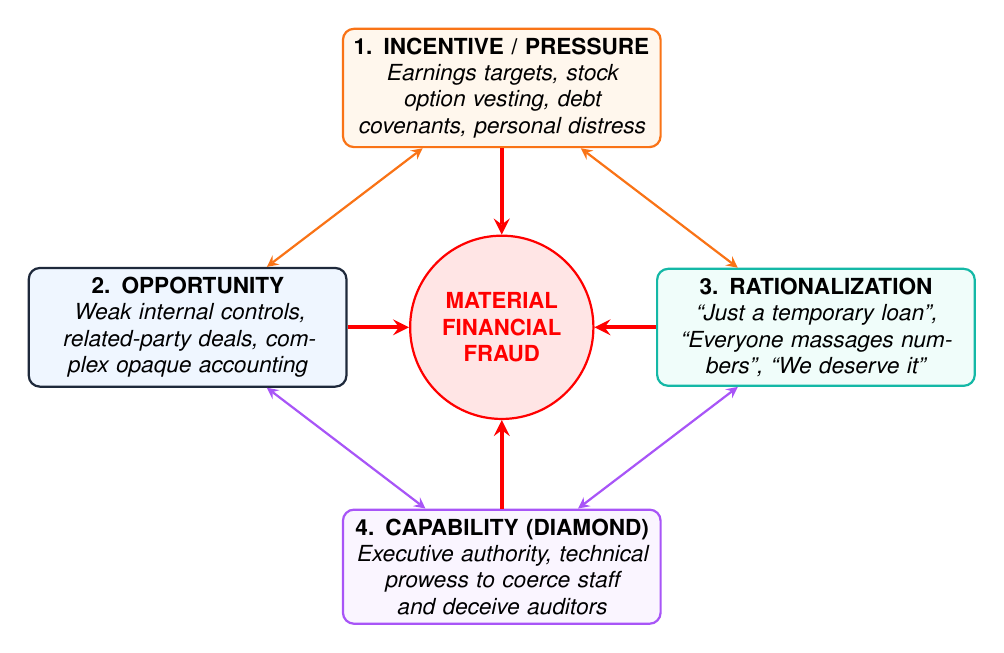
\begin{tikzpicture}[
    scale=0.95,
    font=\sffamily\footnotesize,
    node distance=2.2cm,
    every node/.style={align=center}
]

% Diamond Nodes
\node[draw=coralborder, fill=coralbg, thick, rounded corners=4pt, text width=3.8cm, minimum height=1.3cm] (pressure) at (0, 3.2) {
    \textbf{1. INCENTIVE / PRESSURE}\\
    \textit{Earnings targets, stock option vesting, debt covenants, personal distress}
};

\node[draw=primarydark, fill=primarylight, thick, rounded corners=4pt, text width=3.8cm, minimum height=1.3cm] (opportunity) at (-4.2, 0) {
    \textbf{2. OPPORTUNITY}\\
    \textit{Weak internal controls, related-party deals, complex opaque accounting}
};

\node[draw=tealborder, fill=tealbg, thick, rounded corners=4pt, text width=3.8cm, minimum height=1.3cm] (rationalization) at (4.2, 0) {
    \textbf{3. RATIONALIZATION}\\
    \textit{``Just a temporary loan'', ``Everyone massages numbers'', ``We deserve it''}
};

\node[draw=purpleborder, fill=purplebg, thick, rounded corners=4pt, text width=3.8cm, minimum height=1.3cm] (capability) at (0, -3.2) {
    \textbf{4. CAPABILITY (DIAMOND)}\\
    \textit{Executive authority, technical prowess to coerce staff and deceive auditors}
};

% Central Target
\node[draw=red, fill=red!10, circle, thick, inner sep=6pt] (fraud) at (0, 0) {
    \textbf{\textcolor{red}{MATERIAL}}\\
    \textbf{\textcolor{red}{FINANCIAL}}\\
    \textbf{\textcolor{red}{FRAUD}}
};

% Arrows
\draw[<->, >=stealth, thick, color=coralborder] (pressure) -- (opportunity);
\draw[<->, >=stealth, thick, color=coralborder] (pressure) -- (rationalization);
\draw[<->, >=stealth, thick, color=purpleborder] (capability) -- (opportunity);
\draw[<->, >=stealth, thick, color=purpleborder] (capability) -- (rationalization);

\draw[->, >=stealth, line width=1.5pt, color=red] (pressure) -- (fraud);
\draw[->, >=stealth, line width=1.5pt, color=red] (opportunity) -- (fraud);
\draw[->, >=stealth, line width=1.5pt, color=red] (rationalization) -- (fraud);
\draw[->, >=stealth, line width=1.5pt, color=red] (capability) -- (fraud);

\end{tikzpicture}
\caption{The Fraud Diamond: Structural Synthesis of Pressure, Opportunity, Rationalization, and Executive Capability.}
\label{fig:fraud_diamond}
\end{figure}

% ----------------------------------------------------------------------
% PART 4: DEEP INTUITION & CONCEPTUAL DERIVATIONS
% ----------------------------------------------------------------------
\section{Deep Intuition \& Conceptual Derivations}

\subsection{The Mechanics of Earnings Manipulation Schemes}
Corporate financial statement manipulation generally follows two distinct strategies:

\subsubsection{1. Cookie-Jar Reserve Accounting}
During exceptionally profitable quarters, management artificially suppresses reported earnings by recognizing inflated estimated accruals (e.g., excessive provisions for bad debts, restructuring reserves, or inventory writedowns):
\begin{align*}
\text{Debit: } & \text{Bad Debt Expense} \quad \text{Rs.~10 Crores} \\
\text{Credit: } & \text{Allowance for Doubtful Accounts (Contra-Asset)} \quad \text{Rs.~10 Crores}
\end{align*}
In future lean quarters, when operating earnings slump, management reverses these reserves directly into income ($\text{Credit: Bad Debt Expense}$ or $\text{Operating Income}$), smoothing corporate performance and giving investors the illusion of low earnings volatility.

\subsubsection{2. Channel Stuffing and Bill-and-Hold Manipulations}
To satisfy aggressive quarterly revenue expectations, sales executives entice distributors to accept bulk orders beyond normal market absorption capacity, offering lenient return privileges, deferred payment terms, or deep price discounts:
\begin{align*}
\text{Debit: } & \text{Accounts Receivable} \quad \text{Rs.~50 Crores} \\
\text{Credit: } & \text{Revenue} \quad \text{Rs.~50 Crores}
\end{align*}
Because the customers hold right of return without economic risk, the transfer of control under IFRS 15 / ASC 606 is incomplete. In the subsequent quarter, massive inventory returns occur, triggering severe top-line collapse.

% ----------------------------------------------------------------------
% PART 5: EXPLICIT GOTCHAS & DIAGNOSTIC MISCONCEPTIONS
% ----------------------------------------------------------------------
\section{Explicit Gotchas \& Diagnostic Misconceptions}

\begin{trapbox}{Gotcha 1: Confusing Liquidity with Solvency}
\textbf{The Trap:} Assuming a firm with a high Current Ratio ($CA/CL > 3.0$) is immune to bankruptcy.\\
\textbf{Forensic Reality:} Current ratio can be heavily contaminated by illiquid, uncollectible, or fictitious current assets. An enterprise carrying Rs.~$100$ Crores in obsolete inventory and Rs.~$80$ Crores in uncollectible receivables against Rs.~$50$ Crores in current payables exhibits a Current Ratio of $3.6$, yet faces catastrophic insolvency when short-term debts mature.
\end{trapbox}

\begin{trapbox}{Gotcha 2: Treating EBITDA as a Proxy for Cash Flow}
\textbf{The Trap:} Evaluating corporate debt service capability using EBITDA ($\EBIT + \text{D\&A}$) under the belief that ``EBITDA equals cash earnings''.\\
\textbf{Forensic Reality:} EBITDA ignores working capital investments (e.g., cash tied up in soaring unpaid customer receivables), mandatory tax outflows, interest payments, and required replacement capital expenditures. As Warren Buffett famously noted: \textit{``Does management think the tooth fairy pays for capital expenditures?''}
\end{trapbox}

\begin{trapbox}{Gotcha 3: The Danger of Common-Size Trend Reversals}
\textbf{The Trap:} Relying exclusively on vertical common-size percentages when top-line revenues are themselves artificially inflated.\\
\textbf{Forensic Reality:} If an executive inflates revenue by $40\%$ through fictitious bill-and-hold invoices, an operating expense line that grew by $30\%$ in absolute terms will deceptively appear to have \textit{shrunk} as a percentage of revenue ($30\% / 140\% < \text{baseline}$). Vertical analysis must always be cross-calibrated against horizontal physical-unit indices.
\end{trapbox}

\begin{trapbox}{Gotcha 4: Rationalization vs.~Intent in Forensic Legal Proceedings}
\textbf{The Trap:} Assuming that proving executive rationalization (e.g., ``the CEO believed the market would recover next quarter'') exonerates the perpetrator of fraudulent misstatement.\\
\textbf{Forensic Reality:} In criminal jurisprudence, rationalization is a psychological enabler, not a legal defense. Intent (\textit{mens rea}) is established by the deliberate act of booking entries known to lack economic substance, regardless of whether the executive hoped to fix the shortfall later.
\end{trapbox}

% ----------------------------------------------------------------------
% PART 6: COMPARATIVE SYNTHESIS & SUMMARY TABLE
% ----------------------------------------------------------------------
\section{Comparative Synthesis \& Summary Table}

Table~\ref{tab:comparison_fraud_categories} compares the three core branches of the ACFE Fraud Tree across frequency, median financial loss, detection mechanisms, and algorithmic forensic signals.

\begin{table}[htbp]
\centering
\small
\begin{tabularx}{\textwidth}{lXXX}
\toprule
\textbf{Forensic Metric} & \textbf{Asset Misappropriation} & \textbf{Corruption Schemes} & \textbf{Financial Statement Fraud} \\
\midrule
\textbf{Incidence Rate} & Most frequent ($\approx 85\%$ of corporate fraud cases). & Intermediate frequency ($\approx 35\%$ of corporate fraud cases). & Least frequent ($\approx 10\%$ of corporate fraud cases). \\
\addlinespace
\textbf{Median Financial Loss} & Smallest loss ($\approx \$100{,}000$ median loss per scheme). & Moderate loss ($\approx \$250{,}000$ median loss per scheme). & Catastrophic loss ($\approx \$1{,}000{,}000+$ to enterprise collapse). \\
\addlinespace
\textbf{Primary Perpetrators} & Lower-level staff, payroll clerks, procurement officers. & Middle management, purchasing agents, contract negotiators. & C-Suite executives (CEO, CFO, Controllers, Board Promoters). \\
\addlinespace
\textbf{Core Mechanism} & Ghost employees, skimming cash, billing schemes, theft of inventory. & Bribery, kickbacks, conflicts of interest, illegal bid rigging. & Fictitious revenues, hidden liabilities, cookie jars, asset overvaluation. \\
\addlinespace
\textbf{Forensic Analytics} & Duplicate payments, ghost vendor phone/address matches. & Vendor concentration analysis, shell company beneficial ownership graph. & Horizontal/vertical statement variances, Beneish M-Score, accrual divergences. \\
\bottomrule
\end{tabularx}
\caption{Systemic Comparison of Corporate Fraud Categories (ACFE Taxonomy).}
\label{tab:comparison_fraud_categories}
\end{table}

% ----------------------------------------------------------------------
% PART 7: PYTHON / SCIENTIFIC COMPUTING LAB
% ----------------------------------------------------------------------
\section{Python / Scientific Computing Lab: Vertical \& Horizontal Statement Engine}

Listing~\ref{lst:financial_statement_analysis} provides an automated Python engine for processing multi-year financial statements, computing common-size distributions, evaluating horizontal expansion rates, and highlighting divergence red flags.

\begin{lstlisting}[language=Python, caption={Vertical and Horizontal Financial Statement Analysis in Python}, label={lst:financial_statement_analysis}]
import pandas as pd
import numpy as np

def analyze_financial_statements(fs_df: pd.DataFrame, revenue_col: str = 'Revenue') -> pd.DataFrame:
    """
    Performs forensic vertical (common-size) and horizontal (YoY growth) 
    analysis on multi-year financial statement items.
    
    Parameters:
        fs_df (pd.DataFrame): DataFrame indexed by line items, with fiscal year columns.
        revenue_col (str): Line item name representing total scale baseline.
        
    Returns:
        pd.DataFrame: Augmented DataFrame with vertical shares, growth rates, and flags.
    """
    years = [col for col in fs_df.columns if col.startswith('FY')]
    years.sort()
    
    results = fs_df.copy()
    
    # 1. Vertical Analysis (Common-Size % of Revenue)
    for yr in years:
        total_rev = fs_df.loc[revenue_col, yr]
        results[f'{yr}_Vertical%'] = (fs_df[yr] / total_rev * 100.0).round(2)
        
    # 2. Horizontal Analysis (Year-over-Year % Growth)
    for i in range(1, len(years)):
        prev_yr, curr_yr = years[i-1], years[i]
        results[f'YoY_Growth_{curr_yr}%'] = (
            (fs_df[curr_yr] - fs_df[prev_yr]) / fs_df[prev_yr] * 100.0
        ).round(2)
        
    # 3. Forensic Divergence Check: Flag AR growth exceeding Revenue growth by > 15%
    if 'Accounts_Receivable' in fs_df.index:
        for i in range(1, len(years)):
            prev_yr, curr_yr = years[i-1], years[i]
            rev_growth = results.loc[revenue_col, f'YoY_Growth_{curr_yr}%']
            ar_growth = results.loc['Accounts_Receivable', f'YoY_Growth_{curr_yr}%']
            
            flag_col = f'Flag_AR_Divergence_{curr_yr}'
            results[flag_col] = False
            if (ar_growth - rev_growth) > 15.0:
                results.loc['Accounts_Receivable', flag_col] = True
                
    return results

# -------------------------------------------------------------
# Test Dataset with Channel Stuffing Anomaly
# -------------------------------------------------------------
if __name__ == '__main__':
    statement_data = {
        'FY2023': [1000.0, 600.0, 400.0, 150.0, 250.0, 120.0, 50.0],
        'FY2024': [1100.0, 660.0, 440.0, 165.0, 275.0, 140.0, 55.0],
        'FY2025': [1250.0, 720.0, 530.0, 180.0, 350.0, 260.0, 45.0]  # AR spikes to 260!
    }
    line_items = [
        'Revenue', 'COGS', 'Gross_Profit', 'SG&A', 'EBIT', 
        'Accounts_Receivable', 'Operating_Cash_Flow'
    ]
    df = pd.DataFrame(statement_data, index=line_items)
    audit_report = analyze_financial_statements(df)
    
    print("Forensic Vertical and Horizontal Analysis:")
    print(audit_report[['FY2024_Vertical%', 'FY2025_Vertical%', 'YoY_Growth_FY2025%']])
    if 'Flag_AR_Divergence_FY2025' in audit_report.columns:
        print("\nAR Divergence Flagged in FY2025:", 
              audit_report.loc['Accounts_Receivable', 'Flag_AR_Divergence_FY2025'])
\end{lstlisting}

% ----------------------------------------------------------------------
% PART 8: COMPREHENSIVE PRACTICE PROBLEMS
% ----------------------------------------------------------------------
\section{Comprehensive Practice Problems}
\textit{Complete mathematical derivations and diagnostic MCQ distractor rationales are located in the Appendix.}

\subsection*{Part A: Analytical \& Computational Problems}

\begin{enumerate}[label=\textbf{P2.\arabic*}]
    \item \textbf{Multi-Step Income Statement Reconciliation:}\\
    An Indian telecommunications enterprise presents the following trial balance extracts for the financial year (all figures in Rs.~Crores):
    \begin{center}
    \begin{tabular}{lr|lr}
    \toprule
    \textbf{Account} & \textbf{Debit} & \textbf{Account} & \textbf{Credit} \\
    \midrule
    Gross Sales Revenue & --- & Gross Sales Revenue & $2{,}400$ \\
    Sales Returns \& Allowances & $80$ & Non-Operating Interest Income & $35$ \\
    Cost of Goods Sold (COGS) & $1{,}240$ & Gain on Disposal of Tower Assets & $25$ \\
    Administrative Expenses & $220$ & Equity Capital & $500$ \\
    Sales \& Marketing Expenses & $180$ & Long-Term Debt ($9\%$ coupon) & $400$ \\
    Depreciation on Capital Assets & $140$ & Trade Payables & $190$ \\
    Corporate Income Tax Expense ($25\%$) & ? & Retained Earnings & $750$ \\
    \bottomrule
    \end{tabular}
    \end{center}
    \begin{enumerate}[label=(\alph*)]
        \item Compute Net Sales Revenue, Gross Profit, and Operating Profit (EBIT).
        \item Compute EBITDA and Net Profit After Tax.
        \item If management capitalized Rs.~$60$ Crores of marketing costs into intangible assets during the year, reconstruct true EBIT and quantify the percentage overstatement.
    \end{enumerate}

    \item \textbf{Working Capital \& Window Dressing Forensics:}\\
    At fiscal year-end (March 30), a consumer electronics firm reports Current Assets of Rs.~$60{,}00{,}000$ and Current Liabilities of Rs.~$30{,}00{,}000$ (Current Ratio $= 2.0$). To satisfy a bank loan covenant requiring a Current Ratio $\ge 2.2$, the CFO borrows Rs.~$20{,}00{,}000$ in short-term bank overdraft on March 31 and uses Rs.~$15{,}00{,}000$ of available cash to settle trade payables.
    \begin{enumerate}[label=(\alph*)]
        \item Compute the final Current Ratio on March 31 following these actions.
        \item Did the CFO's actions successfully meet the covenant threshold?
        \item Explain why paying off liabilities with cash mathematically improves a Current Ratio that is initially greater than $1.0$.
    \end{enumerate}

    \item \textbf{Common-Size Horizontal Forensic Analysis:}\\
    Over a three-year period, a pharmaceutical company reports the following financial figures (in Rs.~Lakhs):
    \begin{center}
    \begin{tabular}{lrrr}
    \toprule
    \textbf{Metric} & \textbf{Year 1} & \textbf{Year 2} & \textbf{Year 3} \\
    \midrule
    Sales Revenue & $5{,}000$ & $5{,}800$ & $6{,}400$ \\
    Accounts Receivable & $600$ & $950$ & $1{,}600$ \\
    Inventory & $800$ & $1{,}100$ & $1{,}750$ \\
    Allowance for Bad Debts & $60$ & $40$ & $30$ \\
    \bottomrule
    \end{tabular}
    \end{center}
    \begin{enumerate}[label=(\alph*)]
        \item Compute the horizontal percentage growth of Sales, Accounts Receivable, and Inventory from Year 1 to Year 3.
        \item Calculate the Days Sales Outstanding (DSO) for each year assuming a 365-day year.
        \item Analyze the forensic red flags revealed by the trajectory of the Allowance for Bad Debts relative to Receivables.
    \end{enumerate}

    \item \textbf{The Fraud Diamond in Corporate Governance:}\\
    Evaluate the Enron collapse through the lens of the Fraud Diamond. Provide concrete historical evidence illustrating how Incentive, Opportunity, Rationalization, and Capability manifested among Enron's senior leadership (Ken Lay, Jeff Skilling, and Andy Fastow).

    \item \textbf{Off-Balance Sheet Debt \& Operating Leases:}\\
    Prior to IFRS 16 / ASC 842, an airline entered into long-term aircraft operating leases requiring annual lease payments of Rs.~$100$ Crores for the next 10 years. The company's incremental borrowing cost is $8\%$.
    \begin{enumerate}[label=(\alph*)]
        \item Calculate the unrecorded present value of off-balance sheet lease commitments.
        \item Explain how keeping these obligations off the balance sheet distorted the firm's Debt-to-Equity and Return-on-Assets ratios.
    \end{enumerate}
\end{enumerate}

\subsection*{Part B: Diagnostic Multiple-Choice Questions}

\begin{enumerate}[label=\textbf{MCQ 2.\arabic*}]
    \item A manufacturing enterprise artificially inflates its reported Gross Profit margin during Year 2. Forensic investigation reveals that physical production volumes remained constant, unit selling prices did not change, and raw material costs were steady. Which of the following accounting maneuvers directly produces this fraudulent outcome?
    \begin{enumerate}[label=(\alph*)]
        \item Improperly shifting closing inventory valuation from FIFO to a fictitious higher ending inventory balance.
        \item Reclassifying administrative office utility expenses into factory selling expenses.
        \item Writing off obsolete spare parts as an extraordinary impairment loss in the income statement.
        \item Accelerating depreciation on executive office headquarters from straight-line to double-declining balance.
    \end{enumerate}

    \item In the context of the Fraud Diamond, which factor distinguishes Wolfe and Hermanson's model from Cressey's classical Fraud Triangle?
    \begin{enumerate}[label=(\alph*)]
        \item The presence of external financial pressure, such as impending debt covenant defaults.
        \item Executive capability, encompassing technical skill, interpersonal influence, and authoritarian access required to execute and conceal deceit.
        \item Moral rationalization by the perpetrator that the stolen funds are merely a short-term loan.
        \item Deficiencies in corporate governance and an absence of segregation of duties.
    \end{enumerate}
\end{enumerate}

\chapter{Cash Flow Statement \& Forensic Accounting Fundamentals}

% ----------------------------------------------------------------------
% PART 1: EXECUTIVE ROADMAP & LEARNING OBJECTIVES
% ----------------------------------------------------------------------
\section{Executive Roadmap \& Learning Objectives}

Cash flow represents the undeniable lifeblood of enterprise operations. While reported net income is subject to significant accounting discretion, accrual timing conventions, and management estimates, cash receipts and disbursements represent empirical bank settlements. However, contrary to common belief among financial analysts, cash flow statements are not immune to manipulation. Forensic accountants must master the mathematical bridges linking accrual net income to operational cash flow and detect deceptive classification shifts designed to artificially burnish Cash Flow from Operations (CFO).

\begin{tcolorbox}[colback=primarylight, colframe=primarydark, title={\textbf{Core Learning Competencies}}]
Upon mastering this chapter, students will be equipped to:
\begin{itemize}
    \item \textbf{Reconcile Accrual Income to Cash Realization:} Construct and audit the tripartite Statement of Cash Flows across Operating (CFO), Investing (CFI), and Financing (CFF) dimensions under the Direct and Indirect methods.
    \item \textbf{Quantify the Sloan Accrual Disconnect:} Calculate cash-flow and balance-sheet accrual ratios to assess earnings quality and evaluate systemic stock price overvaluation risk.
    \item \textbf{Unmask Cash Flow Manipulation Schemes:} Detect quarter-end accounts receivable factoring, vendor payable stretching, and the illegitimate capitalization of operating disbursements into CFI.
    \item \textbf{Structure Professional Forensic Engagements:} Formulate formal engagement scoping letters, establish strict conflict-of-interest firewalls, and execute objective investigative protocols.
    \item \textbf{Navigate Expert Witness Evidentiary Standards:} Apply legal standards of expert admissibility (Daubert and Frye doctrines) and maintain expert independence under cross-examination.
\end{itemize}
\end{tcolorbox}

\begin{table}[htbp]
\centering
\small
\begin{tabularx}{\textwidth}{llX}
\toprule
\textbf{Financial Symbol} & \textbf{Forensic Construct} & \textbf{Mathematical Definition / Formula} \\
\midrule
$\text{CFO}$ & Cash Flow from Operations & Physical cash generated from primary core commercial activities \\
$\text{CFI}$ & Cash Flow from Investing & Cash inflows/outflows from productive capital assets and securities \\
$\text{CFF}$ & Cash Flow from Financing & Cash flows with debt holders and equity capital providers \\
$\Delta \text{Cash}$ & Net Change in Cash & $\text{CFO} + \text{CFI} + \text{CFF}$ \\
$\text{FCFF}$ & Free Cash Flow to Firm & $\text{CFO} - \text{CapEx}$ \\
$NOA_t$ & Net Operating Assets & $(\text{Total Assets} - \text{Cash}) - (\text{Total Liabilities} - \text{Total Debt})$ \\
$AR_{\text{CF}}$ & Cash Flow Accrual Ratio & $\frac{NI_t - \text{CFO}_t}{(A_t + A_{t-1}) / 2}$ \\
$AR_{\text{BS}}$ & Balance Sheet Accrual Ratio & $\frac{NOA_t - NOA_{t-1}}{(A_t + A_{t-1}) / 2}$ \\
\bottomrule
\end{tabularx}
\caption{Mathematical Notation Guide for Cash Flow and Accruals Forensics.}
\label{tab:w3_notation}
\end{table}

% ----------------------------------------------------------------------
% PART 2: MATHEMATICAL & COMPUTATIONAL FOUNDATIONS
% ----------------------------------------------------------------------
\section{Mathematical \& Computational Foundations}

\subsection{The Tripartite Cash Flow Model}
At any reporting period ending at time $t$, the net movement in an enterprise's cash and cash equivalents ($\Delta \text{Cash}_t$) is decomposed into three mutually exclusive operational flows:
\begin{equation}
\Delta \text{Cash}_t = \text{Cash}_t - \text{Cash}_{t-1} = \text{CFO}_t + \text{CFI}_t + \text{CFF}_t
\label{eq:cash_tripartite}
\end{equation}

\subsection{The Indirect Reconciliatory Formulation}
Under the Indirect Method (codified under IAS 7 / ASC 230), CFO begins with reported Net Income and reverses non-cash expenses, non-operating transaction gains/losses, and operating working capital changes:
\begin{equation}
\text{CFO}_t = NI_t + \sum_{k=1}^m \text{NCC}_{k,t} - \sum_{j=1}^p \text{NonOpGain}_{j,t} - \Delta NOWC_t
\label{eq:indirect_cfo}
\end{equation}
Expanding operating working capital shifts:
\begin{align}
\Delta NOWC_t &= (\Delta \text{Accounts Receivable}_t + \Delta \text{Inventory}_t + \Delta \text{Prepaid Expenses}_t) \nonumber \\
&\quad - (\Delta \text{Accounts Payable}_t + \Delta \text{Accrued Expenses}_t)
\end{align}

\subsection{The Sloan Accrual Anomaly and Earnings Quality}
In 1996, Richard Sloan empirically established that corporate earnings comprised of high non-cash accruals exhibit substantially lower persistence and higher future earnings reversal rates than earnings supported by cash flows.

\begin{definitionbox}{The Cash Flow Accrual Ratio}
\index{Sloan Accrual Ratio}
The Cash Flow Accrual Ratio measures the fraction of operating income unbacked by actual operational cash generation:
\begin{equation}
AR_{\text{CF}, t} = \frac{NI_t - \text{CFO}_t}{\bar{A}_t}, \quad \text{where } \bar{A}_t = \frac{A_t + A_{t-1}}{2}
\label{eq:sloan_accrual}
\end{equation}
\textbf{Forensic Decision Rule:}
\begin{itemize}
    \item $AR_{\text{CF}, t} \le 0$: High earnings quality (CFO meets or exceeds Net Income).
    \item $0 < AR_{\text{CF}, t} \le +0.10$: Normal working capital accrual expansion.
    \item $AR_{\text{CF}, t} > +0.10$: \textcolor{red}{\textbf{Severe Accrual Disconnect}} (high risk of artificial earnings inflation).
\end{itemize}
\end{definitionbox}

% ----------------------------------------------------------------------
% PART 3: VISUAL & GEOMETRIC INTUITION
% ----------------------------------------------------------------------
\section{Visual \& Geometric Intuition: The Cash Flow Waterfall}

Figure~\ref{fig:cash_waterfall} visualizes the indirect transformation of accrual Net Income into operational cash, highlighting where management exploits classification loopholes.

\begin{figure}[htbp]
\centering
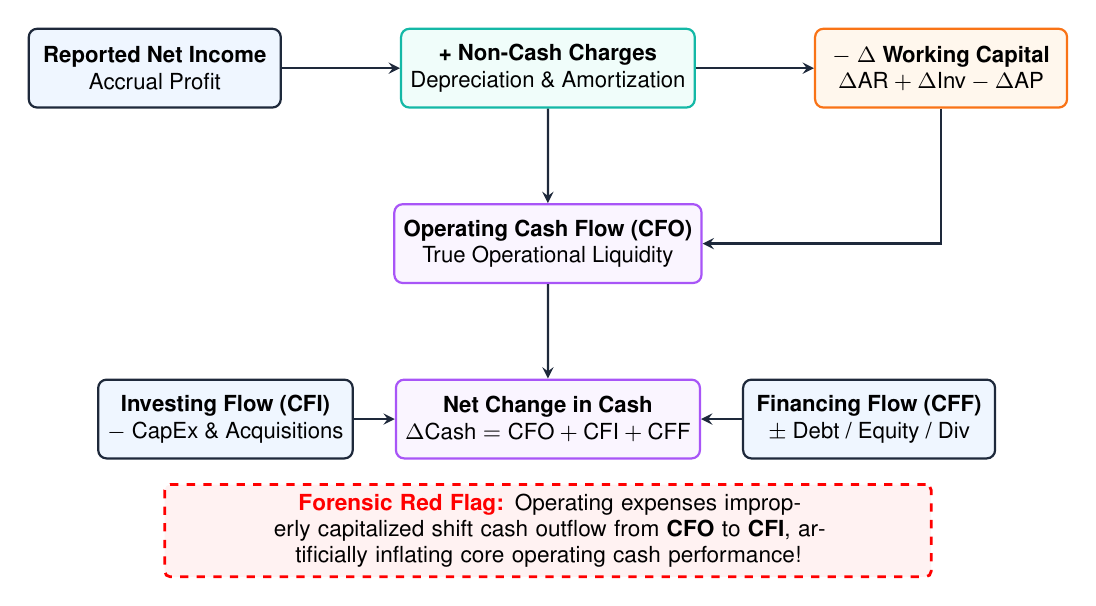
\begin{tikzpicture}[
    scale=0.9,
    font=\sffamily\footnotesize,
    node distance=1.2cm and 1.5cm,
    block/.style={rectangle, draw=primarydark, fill=primarylight, thick, rounded corners=3pt, minimum width=3.2cm, minimum height=1.0cm, align=center},
    add/.style={rectangle, draw=tealborder, fill=tealbg, thick, rounded corners=3pt, minimum width=3.2cm, minimum height=1.0cm, align=center},
    sub/.style={rectangle, draw=coralborder, fill=coralbg, thick, rounded corners=3pt, minimum width=3.2cm, minimum height=1.0cm, align=center},
    target/.style={rectangle, draw=purpleborder, fill=purplebg, thick, rounded corners=3pt, minimum width=3.2cm, minimum height=1.0cm, align=center},
    arr/.style={->, >=stealth, thick, color=primarydark}
]

% Nodes
\node[block] (ni) {\textbf{Reported Net Income}\\Accrual Profit};
\node[add, right=of ni] (dep) {\textbf{+ Non-Cash Charges}\\Depreciation \& Amortization};
\node[sub, right=of dep] (wc) {\textbf{$-$ $\Delta$ Working Capital}\\$\Delta \text{AR} + \Delta \text{Inv} - \Delta \text{AP}$};
\node[target, below=1.2cm of dep] (cfo) {\textbf{Operating Cash Flow (CFO)}\\True Operational Liquidity};

\node[block, below left=1.2cm and 0.5cm of cfo] (cfi) {\textbf{Investing Flow (CFI)}\\$-$ CapEx \& Acquisitions};
\node[block, below right=1.2cm and 0.5cm of cfo] (cff) {\textbf{Financing Flow (CFF)}\\$\pm$ Debt / Equity / Div};
\node[target, below=1.2cm of cfo] (net) {\textbf{Net Change in Cash}\\$\Delta \text{Cash} = \text{CFO} + \text{CFI} + \text{CFF}$};

% Arrows
\draw[arr] (ni) -- (dep);
\draw[arr] (dep) -- (wc);
\draw[arr] (wc) |- (cfo);
\draw[arr] (dep) -- (cfo);
\draw[arr] (cfo) -- (net);
\draw[arr] (cfi) -- (net);
\draw[arr] (cff) -- (net);

% Forensic manipulation warning
\node[draw=red, dashed, line width=1pt, rounded corners=2pt, fill=red!5, below=0.3cm of net, text width=9.5cm, align=center] {
    \textcolor{red}{\textbf{Forensic Red Flag:}} Operating expenses improperly capitalized shift cash outflow from \textbf{CFO} to \textbf{CFI}, artificially inflating core operating cash performance!
};

\end{tikzpicture}
\caption{The Indirect Cash Flow Conversion Architecture and Capitalization Arbitrage.}
\label{fig:cash_waterfall}
\end{figure}

% ----------------------------------------------------------------------
% PART 4: DEEP INTUITION & CONCEPTUAL DERIVATIONS
% ----------------------------------------------------------------------
\section{Deep Intuition \& Conceptual Derivations}

\subsection{Forensic Classification Games within Cash Flows}
Corporate executives under intense market pressure cannot easily falsify the ending cash balance, as it is directly auditable against independent bank confirmations. Instead, they manipulate the \textbf{internal classification} of cash streams between CFO, CFI, and CFF:

\subsubsection{1. Capitalizing Operating Disbursements}
When a company spends cash on routine operating maintenance, the proper entry is:
\begin{align*}
\text{Debit: } & \text{Maintenance Expense} \quad \text{Rs.~50 Crores} \\
\text{Credit: } & \text{Cash} \quad \text{Rs.~50 Crores} \implies \text{Reduces CFO by Rs.~50 Crores}
\end{align*}
If management instead fraudulently capitalizes this disbursement as an asset enhancement:
\begin{align*}
\text{Debit: } & \text{Property, Plant \& Equipment} \quad \text{Rs.~50 Crores} \\
\text{Credit: } & \text{Cash} \quad \text{Rs.~50 Crores} \implies \text{Recorded as CFI (CapEx), leaving CFO untouched!}
\end{align*}
This single classification sleight-of-hand overstates reported Operating Cash Flow by Rs.~$50$ Crores!

\subsubsection{2. Non-Recourse Receivables Factoring at Quarter-End}
To camouflage deteriorating customer collections, an enterprise sells Rs.~$100$ Crores of uncollected customer receivables to a commercial bank two days before fiscal year-end with $10\%$ discount ($90$ Crores cash received). This generates an immediate cash inflow in CFO, temporarily reducing Days Sales Outstanding (DSO). If the transaction is quietly reversed or repurchased in the first week of the new fiscal period, it represents artificial window-dressing.

% ----------------------------------------------------------------------
% PART 5: EXPLICIT GOTCHAS & DIAGNOSTIC MISCONCEPTIONS
% ----------------------------------------------------------------------
\section{Explicit Gotchas \& Diagnostic Misconceptions}

\begin{trapbox}{Gotcha 1: Believing That Cash Flow Cannot Be Falsified}
\textbf{The Trap:} Assuming that because ``cash is fact and profit is opinion'', the Cash Flow from Operations (CFO) is inherently tamper-proof.\\
\textbf{Forensic Reality:} CFO can be aggressively manipulated through:
\begin{enumerate*}[label=(\roman*)]
    \item Disguising bank debt as customer financing advances,
    \item Delaying vendor invoice settlements until the first day of the new quarter,
    \item Selling receivables with unrecorded buyback commitments,
    \item Capitalizing operational software engineering payroll costs into CFI.
\end{enumerate*}
\end{trapbox}

\begin{trapbox}{Gotcha 2: Confusing CFO with Free Cash Flow (FCFF)}
\textbf{The Trap:} Treating a company with robust CFO as financially self-sustaining without factoring in essential capital reinvestment.\\
\textbf{Forensic Reality:} An infrastructure or semiconductor firm generating Rs.~$500$ Crores in CFO while requiring Rs.~$750$ Crores in annual replacement capital expenditures ($\text{CapEx}$) generates \textit{negative} Free Cash Flow ($\text{FCFF} = -\text{Rs.~}250\text{ Crores}$). It must continually issue new debt or equity to survive.
\end{trapbox}

\begin{trapbox}{Gotcha 3: The Hazard of Negative Accrual Ratios in Distressed Turnarounds}
\textbf{The Trap:} Believing that a highly negative accrual ratio ($AR_{\text{CF}} \ll 0$) is unequivocally positive evidence of outstanding earnings health.\\
\textbf{Forensic Reality:} Extreme negative accrual ratios can occur when a dying enterprise liquidates its inventory and halts raw material replenishment, generating a temporary surge in cash inflow as it shrinks toward liquidation.
\end{trapbox}

\begin{trapbox}{Gotcha 4: The Expert Witness Advocacy Trap}
\textbf{The Trap:} Believing that a forensic accountant hired by a legal defense team should act as an aggressive advocate for the client's commercial position.\\
\textbf{Forensic Reality:} Under established evidentiary jurisprudence (including the \textit{Daubert} standard and Federal Rule of Evidence 702), an expert witness owes their primary duty to the court as an objective, independent finder of scientific fact. A forensic accountant who abandons neutrality to become an advocate will be disqualified and their testimony discarded.
\end{trapbox}

% ----------------------------------------------------------------------
% PART 6: COMPARATIVE SYNTHESIS & SUMMARY TABLE
% ----------------------------------------------------------------------
\section{Comparative Synthesis \& Summary Table}

Table~\ref{tab:comparison_cfo_methods} compares the Direct and Indirect methods of cash flow reporting alongside the legal frameworks governing forensic expert witness admissibility.

\begin{table}[htbp]
\centering
\small
\begin{tabularx}{\textwidth}{lXX}
\toprule
\textbf{Dimension} & \textbf{Direct Method (Operating Cash Flows)} & \textbf{Indirect Method (Operating Cash Flows)} \\
\midrule
\textbf{Reporting Mechanism} & Lists gross physical cash collections from customers and gross cash paid to suppliers/employees. & Begins with accrual Net Income and systematically adjusts for non-cash expenses and working capital shifts. \\
\addlinespace
\textbf{Diagnostic Value} & Immediately reveals gross operational cash velocity and actual cash settlement trends. & Directly illuminates the magnitude of the accrual-cash disconnect ($NI - \text{CFO}$). \\
\addlinespace
\textbf{Corporate Adoption} & Rarely adopted voluntarily due to higher ERP accounting system implementation costs. & Universal standard adopted by over $95\%$ of global listed corporations. \\
\addlinespace
\textbf{Forensic Vulnerability} & Misclassifying non-operating receipts into operational customer collection lines. & Arbitrary capitalization of operational outflows into investing activities (CFI). \\
\midrule
\textbf{Legal Evidentiary Rule} & \textbf{Frye Standard (General Acceptance)} & \textbf{Daubert Standard (Scientific Reliability)} \\
\midrule
\textbf{Core Criterion} & Methodology must be generally accepted as reliable by the relevant scientific community. & Judge acts as gatekeeper: testability, peer review, error rates, and professional standards. \\
\bottomrule
\end{tabularx}
\caption{Comparative Synthesis of Cash Flow Reporting Methods and Forensic Admissibility Standards.}
\label{tab:comparison_cfo_methods}
\end{table}

% ----------------------------------------------------------------------
% PART 7: PYTHON / SCIENTIFIC COMPUTING LAB
% ----------------------------------------------------------------------
\section{Python / Scientific Computing Lab: Sloan Accrual \& Earnings Quality Engine}

Listing~\ref{lst:accrual_engine} provides a complete, production-ready Python program that ingests multi-year corporate financials, computes cash-flow and balance-sheet accrual ratios, and flags high-risk divergence periods.

\begin{lstlisting}[language=Python, caption={Sloan Accrual Ratio \& Earnings Quality Analyzer in Python}, label={lst:accrual_engine}]
import pandas as pd
import numpy as np

def compute_accrual_metrics(data: pd.DataFrame) -> pd.DataFrame:
    """
    Computes Sloan Cash Flow and Balance Sheet Accrual Ratios 
    to evaluate corporate earnings persistence and quality.
    
    Parameters:
        data (pd.DataFrame): Financial records with columns ['Year', 'Assets', 
                             'Cash', 'Liabilities', 'Debt', 'Net_Income', 'CFO']
                             
    Returns:
        pd.DataFrame: Augmented metrics containing Accrual Ratios and Forensic Flags.
    """
    df = data.sort_values('Year').copy()
    
    # 1. Compute Average Total Assets
    df['Avg_Assets'] = (df['Assets'] + df['Assets'].shift(1)) / 2.0
    
    # 2. Cash Flow Accrual Ratio: (Net Income - CFO) / Avg Assets
    df['Accrual_CF'] = (df['Net_Income'] - df['CFO']) / df['Avg_Assets']
    
    # 3. Net Operating Assets (NOA): (Assets - Cash) - (Liabilities - Debt)
    df['NOA'] = (df['Assets'] - df['Cash']) - (df['Liabilities'] - df['Debt'])
    df['Delta_NOA'] = df['NOA'].diff()
    
    # Balance Sheet Accrual Ratio: Delta NOA / Avg Assets
    df['Accrual_BS'] = df['Delta_NOA'] / df['Avg_Assets']
    
    # 4. Forensic Red Flag Classification
    # Threshold: Accrual Ratio > +0.10 indicates aggressive earnings disconnect
    df['Flag_CF_Accrual'] = df['Accrual_CF'] > 0.10
    df['Flag_BS_Accrual'] = df['Accrual_BS'] > 0.10
    
    return df

# -------------------------------------------------------------
# Test Harness with Historical Manipulation Scenario
# -------------------------------------------------------------
if __name__ == '__main__':
    records = {
        'Year': [2021, 2022, 2023, 2024, 2025],
        'Assets': [1000.0, 1150.0, 1380.0, 1720.0, 2100.0],
        'Cash': [120.0, 110.0, 95.0, 60.0, 40.0],
        'Liabilities': [450.0, 520.0, 640.0, 830.0, 1050.0],
        'Debt': [200.0, 250.0, 320.0, 450.0, 600.0],
        'Net_Income': [110.0, 140.0, 185.0, 260.0, 340.0],
        'CFO': [115.0, 130.0, 110.0, 75.0, 30.0]  # Severe CFO collapse!
    }
    
    df_corp = pd.DataFrame(records)
    results = compute_accrual_metrics(df_corp)
    
    output_cols = ['Year', 'Net_Income', 'CFO', 'Accrual_CF', 'Accrual_BS', 'Flag_CF_Accrual']
    print("Forensic Earnings Quality & Accrual Audit:")
    print(results[output_cols].to_string(index=False))
\end{lstlisting}

% ----------------------------------------------------------------------
% PART 8: COMPREHENSIVE PRACTICE PROBLEMS
% ----------------------------------------------------------------------
\section{Comprehensive Practice Problems}
\textit{Complete mathematical derivations and diagnostic MCQ distractor rationales are located in the Appendix.}

\subsection*{Part A: Analytical \& Computational Problems}

\begin{enumerate}[label=\textbf{P3.\arabic*}]
    \item \textbf{Indirect Method Cash Flow Construction:}\\
    An industrial automation firm reports Net Income of Rs.~$8{,}40{,}000$ for the fiscal year ending March 31. Additional accounting records provide the following information:
    \begin{itemize}
        \item Depreciation on plant and machinery: Rs.~$1{,}90{,}000$.
        \item Amortization of software patents: Rs.~$45{,}000$.
        \item Profit on sale of surplus industrial land: Rs.~$60{,}000$.
        \item Trade Accounts Receivable increased by Rs.~$1{,}20{,}000$.
        \item Raw material and finished goods inventory decreased by Rs.~$75{,}000$.
        \item Trade Accounts Payable increased by Rs.~$50{,}000$.
        \item Accrued employee salaries payable decreased by Rs.~$30{,}000$.
    \end{itemize}
    \begin{enumerate}[label=(\alph*)]
        \item Calculate Cash Flow from Operating Activities (CFO) under the Indirect Method.
        \item Explain why the gain on land disposal is subtracted from Net Income in calculating CFO.
        \item If the firm purchased new robotic assembly equipment for Rs.~$4{,}00{,}000$, compute the Free Cash Flow to Firm (FCFF).
    \end{enumerate}

    \item \textbf{Sloan Accrual Ratio \& Manipulation Scoring:}\\
    A publicly listed retail chain reports the following balance sheet and operating data over two consecutive fiscal years (in Rs.~Crores):
    \begin{center}
    \begin{tabular}{lrr}
    \toprule
    \textbf{Metric} & \textbf{Year 1} & \textbf{Year 2} \\
    \midrule
    Total Assets & $4{,}000$ & $5{,}200$ \\
    Cash \& Marketable Securities & $400$ & $300$ \\
    Total Liabilities & $1{,}800$ & $2{,}500$ \\
    Total Short-Term \& Long-Term Debt & $800$ & $1{,}200$ \\
    Reported Net Income & $360$ & $520$ \\
    Cash Flow from Operations (CFO) & $380$ & $140$ \\
    \bottomrule
    \end{tabular}
    \end{center}
    \begin{enumerate}[label=(\alph*)]
        \item Compute the Cash Flow Accrual Ratio for Year 2.
        \item Compute the Net Operating Assets (NOA) for Year 1 and Year 2, and determine the Balance Sheet Accrual Ratio.
        \item Formulate a forensic assessment regarding the earnings sustainability of this firm.
    \end{enumerate}

    \item \textbf{Cash Flow Classification Forensics:}\\
    During a financial investigation, you discover that a software firm recorded the following transactions:
    \begin{enumerate}[label=(\alph*)]
        \item Capitalized Rs.~$25$ Crores of routine website bug-fixing payroll costs as ``Intangible Software Development Assets'' (recorded as CapEx in CFI).
        \item Obtained a short-term bank credit line of Rs.~$40$ Crores and recorded the cash inflow under ``Customer Advances'' in Operating Cash Flows.
    \end{enumerate}
    Quantify the artificial inflation in reported CFO and discuss the impact on the firm's perceived operating health.

    \item \textbf{Working Capital Factoring Schemes:}\\
    On December 29, a pharmaceutical company factors Rs.~$80$ Crores of 90-day trade receivables to an independent factoring agency for Rs.~$74$ Crores cash with full recourse (the company must reimburse the factor if customers default). The company derecognizes the receivables and reports Rs.~$74$ Crores in CFO. Evaluate whether derecognition was appropriate under IFRS 9 / ASC 860 and formulate the correct forensic accounting treatment.

    \item \textbf{Evidentiary Standards for Forensic Expert Witnesses:}\\
    In a corporate embezzlement trial, the defense challenges the admissibility of the prosecution's forensic expert report, arguing that the expert utilized proprietary, unpublished machine learning algorithms to detect fraudulent invoices. Analyze this challenge under the \textit{Daubert} standard.
\end{enumerate}

\subsection*{Part B: Diagnostic Multiple-Choice Questions}

\begin{enumerate}[label=\textbf{MCQ 3.\arabic*}]
    \item Which of the following corporate transactions produces an immediate increase in reported Cash Flow from Operations (CFO) under the indirect method while having zero impact on Net Income during the current fiscal period?
    \begin{enumerate}[label=(\alph*)]
        \item Negotiating extended supplier payment terms, leading to a substantial increase in ending Accounts Payable.
        \item Recognizing an extraordinary non-operating gain on the sale of surplus corporate real estate.
        \item Writing off uncollectible customer debts against the pre-existing Allowance for Doubtful Accounts.
        \item Purchasing manufacturing inventory with cash directly from the supplier.
    \end{enumerate}

    \item Under the legal framework established by the United States Supreme Court in \textit{Daubert v. Merrell Dow Pharmaceuticals, Inc.}, which factor is a trial judge mandated to evaluate when determining the admissibility of forensic scientific expert testimony?
    \begin{enumerate}[label=(\alph*)]
        \item Whether the expert witness holds an active equity stake in the plaintiff corporation.
        \item Whether the underlying analytical technique has been tested, subjected to peer review, possesses a known error rate, and maintains established operational standards.
        \item Whether the expert witness agrees to accept a contingency fee tied to the verdict.
        \item Whether the methodology has been explicitly adopted by every statutory auditor in the jurisdiction.
    \end{enumerate}
\end{enumerate}

\chapter{The Forensic Investigation Process \& Cross-Statement Reconciliation}

\begin{tcolorbox}[colback=primarylight, colframe=primarydark, title={\textbf{What You Will Learn in this Chapter}}]
\begin{itemize}
    \item The complete forensic engagement lifecycle: Predication, Scoping, Evidence Gathering, and Reporting
    \item Chain of custody and legal admissibility protocols for digital and paper evidence
    \item Investigative interviewing techniques and cognitive interview frameworks
    \item Inter-statement articulation: Mathematical reconciliation across the three financial statements
    \item Red flag typologies: Round-tripping transactions, hidden related-party deals, and off-balance sheet liabilities
    \item Data Science implementation of cross-statement reconciliation checks
\end{itemize}
\end{tcolorbox}

\section{The Forensic Investigation Lifecycle}

Unlike routine recurring statutory audits, a \index{forensic investigation}\textbf{forensic investigation} is triggered only when there is reasonable justification, known in legal terminology as \index{predication}\textbf{predication}.

\begin{definitionbox}{Predication}
\index{Predication}
Predication is the totality of circumstances, facts, and observations that would lead a reasonable, professionally prudent individual to believe that fraud, embezzlement, or financial misconduct has occurred, is occurring, or will occur. An investigation must never be initiated as a speculative ``fishing expedition'' without valid predication.
\end{definitionbox}

\begin{theorembox}{The Six Phases of a Forensic Investigation}
\begin{enumerate}
    \item \textbf{Predication \& Engagement Acceptance:} Receipt of whistleblower tip, regulatory referral, or anomalous audit finding; conflict-of-interest check; formal engagement letter.
    \item \textbf{Investigation Planning \& Scoping:} Formulating hypotheses, identifying required evidence repositories, defining technical and legal boundaries.
    \item \textbf{Evidence Collection \& Preservation:} Securing digital hard drives, enterprise resource planning (ERP) logs, email communications, and bank statements while maintaining an unbroken chain of custody.
    \item \textbf{Data Analytics \& Substantive Testing:} Applying algorithmic forensic procedures, journal entry testing, reconstructive accounting, and outlier detection.
    \item \textbf{Investigative Interviewing:} Interviewing neutral third parties and corroborative witnesses before conducting confrontation interviews with target subjects.
    \item \textbf{Reporting \& Testimony:} Preparing the comprehensive forensic investigation report and providing expert testimony in criminal/civil proceedings.
\end{enumerate}
\end{theorembox}

\begin{videocard}{IITM BS Lecture: Revisiting Financial Statements -- Part 1}{https://www.youtube.com/watch?v=Kshd51rTjS0}
Revisiting the inter-linkages between corporate balance sheets and operating statements through an audit lens.
\end{videocard}

\begin{videocard}{IITM BS Lecture: Revisiting Financial Statements -- Part 2}{https://www.youtube.com/watch?v=0QY8_CesCoc}
Deep dive into adjustments, accrued liabilities, contingent reserves, and disclosure notes.
\end{videocard}

\section{Evidence Management and Chain of Custody}

In forensic science, physical and electronic records are subject to strict evidentiary scrutiny. If an investigator cannot prove who collected an item of evidence, where it was stored, and that it remained unaltered, the judge will exclude it from trial.

\begin{warningbox}{The Evidentiary Chain of Custody}
\index{Chain of Custody}
For every digital disk image, database export, or document seized:
\begin{itemize}
    \item Record the exact date, time, physical location, and custodian from whom it was acquired.
    \item Generate a cryptographic hash (SHA-256) of electronic evidence immediately upon acquisition.
    \item Work exclusively on bit-stream forensic working copies, never on original source media.
    \item Document every transfer of custody in a formal Chain of Custody Log.
\end{itemize}
\end{warningbox}

\begin{videocard}{IITM BS Lecture: Revisiting Financial Statements -- Part 3}{https://www.youtube.com/watch?v=2vh4Wr7yzbM}
Detailed analysis of working capital distortions, revenue cycle leakage, and audit trails.
\end{videocard}

\begin{videocard}{IITM BS Lecture: Revisiting Financial Statements -- Part 4}{https://www.youtube.com/watch?v=Q_9-lq_wfnY}
Comprehensive case study synthesizing complex multi-year financial statements to isolate accounting irregularities.
\end{videocard}

\section{Inter-Statement Articulation and Reconciliation}

Financial statements do not exist in isolation; they are mathematically bound together through \index{statement articulation}\textbf{statement articulation}:
\begin{enumerate}
    \item \textbf{Net Income} flows directly into \textbf{Retained Earnings} on the Balance Sheet:
    \begin{equation}
    \text{Retained Earnings}_t = \text{Retained Earnings}_{t-1} + \text{Net Income}_t - \text{Dividends}_t
    \end{equation}
    \item \textbf{Cash Flow from Operations} links the accrual Income Statement back to the change in \textbf{Cash and Cash Equivalents} on the Balance Sheet.
    \item \textbf{Depreciation Expense} on the Income Statement ties to \textbf{Accumulated Depreciation} on the Balance Sheet and non-cash add-backs on the Cash Flow Statement.
\end{enumerate}

\begin{figure}[htbp]
\centering
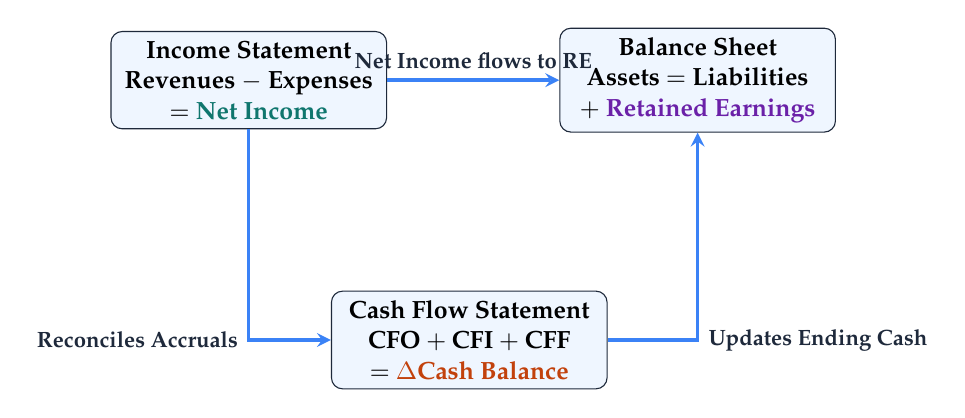
\begin{tikzpicture}[
  node distance=2.5cm,
  stmt/.style={rectangle, draw=primarydark, fill=primarylight, rounded corners, minimum width=3.5cm, minimum height=1.2cm, font=\small\bfseries, align=center},
  flow/.style={->, >=stealth, very thick, primaryborder}
]
\node[stmt] (is) {\textbf{Income Statement}\\Revenues $-$ Expenses\\$=$ \textcolor{tealdef}{Net Income}};
\node[stmt, right of=is, xshift=3.2cm] (bs) {\textbf{Balance Sheet}\\Assets $=$ Liabilities\\$+$ \textcolor{purpleex}{Retained Earnings}};
\node[stmt, below of=is, yshift=-0.8cm, xshift=2.8cm] (cfs) {\textbf{Cash Flow Statement}\\$\text{CFO} + \text{CFI} + \text{CFF}$\\$=$ \textcolor{coralformula}{$\Delta\text{Cash Balance}$}};

\draw[flow] (is) -- node[above, font=\footnotesize\bfseries, color=primarydark] {Net Income flows to RE} (bs);
\draw[flow] (is) |- node[left, font=\footnotesize\bfseries, color=primarydark] {Reconciles Accruals} (cfs);
\draw[flow] (cfs) -| node[right, font=\footnotesize\bfseries, color=primarydark] {Updates Ending Cash} (bs);
\end{tikzpicture}
\caption{Mathematical Inter-Statement Articulation Flow Architecture.}
\end{figure}

\begin{intuitionbox}{Detecting Fabricated Statements via Articulation Invariants}
When fraudsters construct bogus financial statements for loan applications or investor presentations, they frequently alter individual numbers (e.g., arbitrarily inflating revenue and cash) without updating the corresponding contra-accounts or recalculating retained earnings. Testing for mathematical articulation invariants immediately exposes fabricated books.
\end{intuitionbox}

\begin{examplebox}{Historical Case Study: Olympus Corp. ``Tobashi'' Loss-Hiding (2011)}
\index{Olympus Scandal}
Japanese optical equipment giant Olympus concealed over $\$1.5\text{ Billion}$ in investment losses spanning the 1990s and 2000s using a fraudulent practice known as \textit{tobashi} (flying losses away):
\begin{itemize}
    \item \textbf{The Fraudulent Scheme:} To avoid recognizing massive unrealized losses on risky securities during Japan's asset bubble collapse, executives sold the depreciated securities at original inflated book value to off-balance-sheet Cayman and Liechtenstein shell entities funded by loans from Olympus-affiliated banks.
    \item \textbf{The Cover-Up:} Over the next decade, Olympus acquired unrelated shell businesses (e.g., medical waste, face cream makers) at astronomical valuations, paying $\$687\text{ Million}$ in advisory fees to mysterious offshore advisors to secretly funnel cash into the shell entities and settle the hidden bank debts.
    \item \textbf{Forensic Takeaway:} Michael Woodford, the first non-Japanese CEO, blew the whistle after discovering that acquisition advisory fees ($36\%$ of deal value vs.~normal $1-2\%$) completely violated inter-statement sanity checks and M\&A audit benchmarks.
\end{itemize}
\end{examplebox}

\section{Data Science Relevance: Automated Reconciliation Testing}

In a corporate group with dozens of subsidiaries, forensic teams deploy script-based articulation checks across hundreds of entity balance sheets to identify unexplained equity plugs or phantom reserves.

\begin{lstlisting}[caption={Inter-Statement Articulation Checker in Python}]
import pandas as pd

def audit_statement_articulation(financial_panel: pd.DataFrame) -> pd.DataFrame:
    """
    Verifies the fundamental articulation invariants across successive reporting periods:
    1. Retained Earnings Roll-Forward: RE_t = RE_{t-1} + Net_Income_t - Dividends_t
    2. Cash Balance Reconciliation: Cash_t = Cash_{t-1} + Net_Change_Cash_t
    """
    df = financial_panel.copy()
    
    # Lag previous period ending balances
    df['Prev_RE'] = df.groupby('entity_id')['retained_earnings'].shift(1)
    df['Prev_Cash'] = df.groupby('entity_id')['cash'].shift(1)
    
    # Expected Retained Earnings
    df['Expected_RE'] = df['Prev_RE'] + df['net_income'] - df['dividends']
    df['RE_Discrepancy'] = (df['retained_earnings'] - df['Expected_RE']).round(2)
    
    # Expected Cash Balance
    df['Expected_Cash'] = df['Prev_Cash'] + df['cfo'] + df['cfi'] + df['cff']
    df['Cash_Discrepancy'] = (df['cash'] - df['Expected_Cash']).round(2)
    
    # Flag violations
    df['Articulation_Failure'] = (df['RE_Discrepancy'].abs() > 0.01) | (df['Cash_Discrepancy'].abs() > 0.01)
    return df

# Sample audit panel dataset for Subsidiary A
subsidiary_records = pd.DataFrame({
    'entity_id': ['Sub_A', 'Sub_A', 'Sub_A'],
    'year': [2022, 2023, 2024],
    'cash': [100.0, 140.0, 185.0],
    'retained_earnings': [300.0, 360.0, 410.0],
    'net_income': [np.nan, 80.0, 95.0],
    'dividends': [np.nan, 20.0, 30.0],     # In 2024: 360 + 95 - 30 = 425 != 410!
    'cfo': [np.nan, 60.0, 70.0],
    'cfi': [np.nan, -20.0, -35.0],
    'cff': [np.nan, 0.0, 10.0]
})

audit_results = audit_statement_articulation(subsidiary_records)
print(audit_results[['entity_id', 'year', 'RE_Discrepancy', 'Cash_Discrepancy', 'Articulation_Failure']])
\end{lstlisting}

\section{Regulatory Disclosures \& Legal Reporting Protocols}

When forensic reconciliation tests indicate substantive accounting deceit, the investigator must follow formal reporting channels:

\begin{theorembox}{Regulatory Reporting Procedures: Form ADT-4 \& SEBI LODR}
\index{Form ADT-4}\index{SEBI LODR}
\begin{enumerate}
    \item \textbf{Form ADT-4 Escalation Protocol (Ministry of Corporate Affairs):}
    \begin{itemize}
        \item The auditor forwards suspected fraud findings to the company's \textbf{Board of Directors} and \textbf{Audit Committee} seeking their formal reply within 45 days.
        \item On receipt of the reply (or upon expiry of 45 days if no reply is received), the auditor files \textbf{Form ADT-4} directly with the \textbf{Secretary, Ministry of Corporate Affairs (MCA)}, Government of India within 15 days.
    \end{itemize}
    \item \textbf{SEBI LODR Regulation 30 (Listed Companies):}
    Listed entities are legally mandated to make explicit stock exchange disclosures within 24 hours regarding: (1) the initiation of any forensic audit, (2) the reasons for the forensic audit, and (3) the final forensic audit report along with management comments.
\end{enumerate}
\end{theorembox}

\section*{Supplementary Lecture Videos}
\begin{itemize}
    \item \href{https://www.youtube.com/watch?v=Kshd51rTjS0}{W4\_L1: Revisiting Financial Statements -- Part 1 (Audit Adjustments)}
    \item \href{https://www.youtube.com/watch?v=0QY8_CesCoc}{W4\_L2: Revisiting Financial Statements -- Part 2 (Contingent Liabilities)}
    \item \href{https://www.youtube.com/watch?v=2vh4Wr7yzbM}{W4\_L3: Revisiting Financial Statements -- Part 3 (Working Capital Distortions)}
    \item \href{https://www.youtube.com/watch?v=Q_9-lq_wfnY}{W4\_L4: Revisiting Financial Statements -- Part 4 (Full Financial Forensic Synthesis)}
\end{itemize}

\newpage
\section{Practice Exercises}
\textit{Detailed step-by-step solutions are available in the Appendix.}

\begin{enumerate}
    \item Define predication and explain why an anonymous whistleblower allegation containing specific invoice numbers, dates, and bank accounts satisfies the threshold for predication, whereas an anonymous letter stating ``the management is corrupt'' does not.
    
    \item A forensic investigator seizes an accounting department laptop suspected of containing an off-the-books shadow ledger in Microsoft Excel. Outline the step-by-step forensic imaging procedure, explaining write-blockers and cryptographic hashing verification.
    
    \item In auditing the financial statements of Beta Corp., you observe that Retained Earnings at the beginning of 2024 were Rs.~12,50,000. During 2024, the firm reported Net Income of Rs.~4,20,000 and declared cash dividends of Rs.~1,00,000. However, the ending Retained Earnings reported on the December 31, 2024 balance sheet is Rs.~17,80,000. Quantify the reconciliation discrepancy and list three possible fraudulent or erroneous transactions that would produce this imbalance.
    
    \item Explain the concept of a ``round-trip transaction'' (also called ``circular transactions'' or ``swaps''). How do two colluding enterprises artificially inflate top-line revenues without impacting net income or operating cash flows?
    
    \item Compare the objectives and questioning styles of an investigative interview conducted with a neutral third-party witness versus an admission-seeking interview with a target suspect.
\end{enumerate}

\chapter{Financial Ratios, Benford's Law \& Audit Fraud Detection}

% ----------------------------------------------------------------------
% PART 1: EXECUTIVE ROADMAP & LEARNING OBJECTIVES
% ----------------------------------------------------------------------
\section{Executive Roadmap \& Learning Objectives}

Forensic ratio analysis and digital digit distribution analysis represent two foundational quantitative methodologies used to pierce corporate opacity. While financial ratios standardize operational results across scale and expose relational dislocations between operating efficiency, capital structure, and profitability, Benford's Law leverages statistical mechanics to identify anomalous human intervention in financial transaction journals.

\begin{tcolorbox}[colback=primarylight, colframe=primarydark, title={\textbf{Core Learning Competencies}}]
Upon mastering this chapter, students will be equipped to:
\begin{itemize}
    \item \textbf{Deconstruct Corporate Profitability via the DuPont Tree:} Dissect Return on Equity (ROE) into operating profit margin, total asset turnover, and the financial leverage multiplier.
    \item \textbf{Score Earnings Quality with the Beneish M-Score:} Formulate and evaluate the 8-variable probabilistic probit model to calculate financial manipulation probability.
    \item \textbf{Derive Benford's Law Invariants:} Prove the logarithmic probability distribution of leading digits from the principle of scale invariance.
    \item \textbf{Execute Statistical Audit Tests:} Apply Pearson's Chi-Square ($\chi^2$) goodness-of-fit and Mean Absolute Deviation (MAD) against empirical transaction ledgers.
    \item \textbf{Deploy Automated Digit Forensics:} Implement production-ready Python pipelines and Excel functions to flag non-conforming transaction clusters.
\end{itemize}
\end{tcolorbox}

\begin{table}[htbp]
\centering
\small
\begin{tabularx}{\textwidth}{llX}
\toprule
\textbf{Construct / Metric} & \textbf{Symbol} & \textbf{Mathematical Definition / Decision Rule} \\
\midrule
Return on Equity & $\text{ROE}$ & $\frac{\text{Net Income}}{\text{Shareholders' Equity}} = \left(\frac{NI}{\text{Sales}}\right) \times \left(\frac{\text{Sales}}{\text{Assets}}\right) \times \left(\frac{\text{Assets}}{\text{Equity}}\right)$ \\
Beneish M-Score & $M$ & $\boldsymbol{\beta}^T \mathbf{X} > -1.78 \implies \text{High Probability of Manipulation}$ \\
Days Sales Outstanding & $\text{DSO}$ & $\frac{\text{Average Accounts Receivable}}{\text{Net Credit Sales}} \times 365$ \\
Benford 1st-Digit Prob & $P(D_1 = d)$ & $\log_{10}\left(1 + \frac{1}{d}\right) \quad \text{for } d \in \{1, 2, \dots, 9\}$ \\
Benford 2nd-Digit Prob & $P(D_2 = d_2)$ & $\sum_{k=1}^9 \log_{10}\left(1 + \frac{1}{10k + d_2}\right) \quad \text{for } d_2 \in \{0, 1, \dots, 9\}$ \\
Goodness-of-Fit Statistic & $\chi^2$ & $\sum_{d=1}^9 \frac{(O_d - E_d)^2}{E_d} \quad (df = 8)$ \\
Mean Absolute Deviation & $\text{MAD}$ & $\frac{1}{9} \sum_{d=1}^9 |p_d^{\text{obs}} - p_d^{\text{exp}}|$ \\
\bottomrule
\end{tabularx}
\caption{Mathematical Notation Guide for Ratio Decomposition and Benford Forensics.}
\label{tab:w5_notation}
\end{table}

% ----------------------------------------------------------------------
% PART 2: MATHEMATICAL & COMPUTATIONAL FOUNDATIONS
% ----------------------------------------------------------------------
\section{Mathematical \& Computational Foundations}

\subsection{The DuPont 3-Step and 5-Step Decompositions}
Developed by Donaldson Brown at the DuPont Corporation in 1914, the DuPont model separates an enterprise's return on equity into operational, capital efficiency, and leverage dimensions:
\begin{equation}
\text{ROE} = \underbrace{\left(\frac{\text{Net Income}}{\text{Revenue}}\right)}_{\text{Net Profit Margin}} \times \underbrace{\left(\frac{\text{Revenue}}{\text{Total Assets}}\right)}_{\text{Asset Turnover}} \times \underbrace{\left(\frac{\text{Total Assets}}{\text{Shareholders' Equity}}\right)}_{\text{Equity Multiplier}}
\label{eq:dupont_3step}
\end{equation}
The extended 5-step model further isolates operating profit from financing interest burden and corporate taxation:
\begin{equation}
\text{ROE} = \underbrace{\left(\frac{\text{Net Income}}{\text{EBT}}\right)}_{\text{Tax Burden}} \times \underbrace{\left(\frac{\text{EBT}}{\text{EBIT}}\right)}_{\text{Interest Burden}} \times \underbrace{\left(\frac{\text{EBIT}}{\text{Revenue}}\right)}_{\text{Operating Margin}} \times \left(\frac{\text{Revenue}}{\text{Assets}}\right) \times \left(\frac{\text{Assets}}{\text{Equity}}\right)
\label{eq:dupont_5step}
\end{equation}

\subsection{The Beneish M-Score Probabilistic Model}
Formulated by Professor Messod Beneish in 1999, the 8-variable M-Score is a probit model calibrated on known accounting restatement and financial manipulation firms:
\begin{align}
M &= -4.84 + 0.920 \cdot \text{DSRI} + 0.528 \cdot \text{GMI} + 0.404 \cdot \text{AQI} + 0.892 \cdot \text{SGI} \nonumber \\
&\quad + 0.115 \cdot \text{DEPI} - 0.172 \cdot \text{SGAI} + 4.037 \cdot \text{TATA} + 0.0327 \cdot \text{LVGI}
\label{eq:beneish_m}
\end{align}
where:
\begin{itemize}
    \item $\text{DSRI} = \frac{\text{Receivables}_t / \text{Sales}_t}{\text{Receivables}_{t-1} / \text{Sales}_{t-1}}$ (Days Sales in Receivables Index)
    \item $\text{GMI} = \frac{\text{Gross Margin}_{t-1}}{\text{Gross Margin}_t}$ (Gross Margin Deterioration Index)
    \item $\text{AQI} = \frac{1 - (\text{CA}_t + \text{PP\&E}_t + \text{Sec}_t)/\text{Assets}_t}{1 - (\text{CA}_{t-1} + \text{PP\&E}_{t-1} + \text{Sec}_{t-1})/\text{Assets}_{t-1}}$ (Asset Quality Index)
    \item $\text{SGI} = \frac{\text{Sales}_t}{\text{Sales}_{t-1}}$ (Sales Growth Index)
    \item $\text{DEPI} = \frac{\text{DeprRate}_{t-1}}{\text{DeprRate}_t}$ (Depreciation Slowdown Index)
    \item $\text{SGAI} = \frac{\text{SG\&A}_t / \text{Sales}_t}{\text{SG\&A}_{t-1} / \text{Sales}_{t-1}}$ (Sales Overhead Expense Index)
    \item $\text{LVGI} = \frac{\text{Leverage}_t}{\text{Leverage}_{t-1}}$ (Leverage Index)
    \item $\text{TATA} = \frac{\text{Operating Income}_t - \text{CFO}_t}{\text{Total Assets}_t}$ (Total Accruals to Total Assets)
\end{itemize}
\textbf{Decision Threshold:} If $M > -1.78$, the probability of manipulation is statistically elevated ($p > 3.8\%$). In Enron's 2000 financial filings, the Beneish M-Score reached $-1.49$, flagging extensive manipulation prior to bankruptcy.

\subsection{Benford's Law: First and Second-Digit Distributions}
Discovered by Simon Newcomb (1881) and popularized by Frank Benford (1938), Benford's Law describes the natural frequency distribution of leading digits in multi-scale numerical phenomena:
\begin{equation}
P(D_1 = d) = \log_{10}\left(1 + \frac{1}{d}\right) = \log_{10}(d + 1) - \log_{10}(d), \quad d \in \{1, 2, \dots, 9\}
\label{eq:benford_1st}
\end{equation}
The second-digit distribution expands to:
\begin{equation}
P(D_2 = d_2) = \sum_{k=1}^9 \log_{10}\left(1 + \frac{1}{10k + d_2}\right), \quad d_2 \in \{0, 1, \dots, 9\}
\label{eq:benford_2nd}
\end{equation}

% ----------------------------------------------------------------------
% PART 3: VISUAL & GEOMETRIC INTUITION
% ----------------------------------------------------------------------
\section{Visual \& Geometric Intuition: The DuPont Decomposition Tree}

Figure~\ref{fig:dupont_tree} displays the structural hierarchy of Return on Equity, demonstrating how operational profit margins, asset turnover, and balance sheet leverage multiply to determine total equity yield.

\begin{figure}[htbp]
\centering
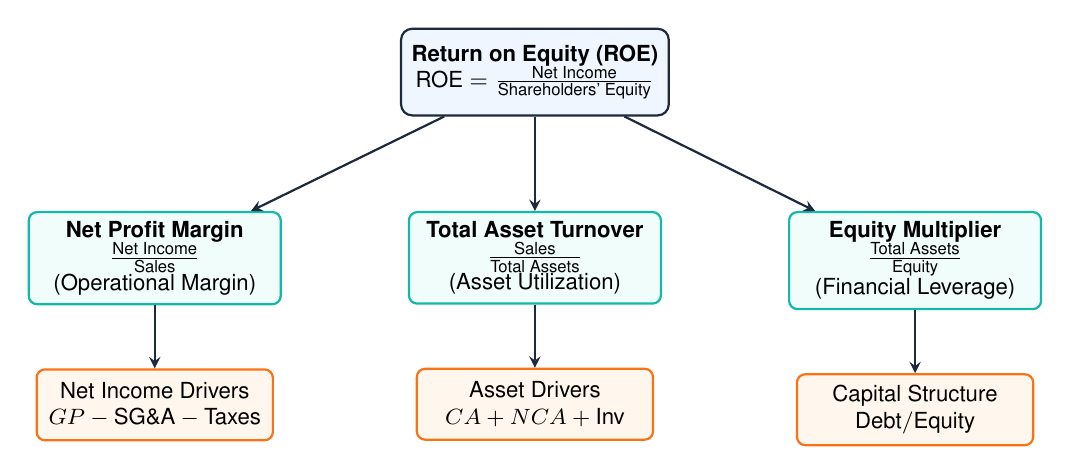
\begin{tikzpicture}[
    font=\sffamily\footnotesize,
    node distance=1.2cm and 1.6cm,
    head/.style={rectangle, draw=primarydark, fill=primarylight, thick, rounded corners=4pt, minimum width=3.4cm, minimum height=1.1cm, align=center},
    dstep/.style={rectangle, draw=tealborder, fill=tealbg, thick, rounded corners=3pt, minimum width=3.2cm, minimum height=1.0cm, align=center},
    leaf/.style={rectangle, draw=coralborder, fill=coralbg, thick, rounded corners=3pt, minimum width=3.0cm, minimum height=0.9cm, align=center},
    arr/.style={->, >=stealth, thick, color=primarydark}
]

% Root
\node[head] (roe) {\textbf{Return on Equity (ROE)}\\$\text{ROE} = \frac{\text{Net Income}}{\text{Shareholders' Equity}}$};

% Level 1
\node[dstep, below left=1.2cm and 1.5cm of roe] (npm) {\textbf{Net Profit Margin}\\$\frac{\text{Net Income}}{\text{Sales}}$\\(Operational Margin)};
\node[dstep, below=1.2cm of roe] (ato) {\textbf{Total Asset Turnover}\\$\frac{\text{Sales}}{\text{Total Assets}}$\\(Asset Utilization)};
\node[dstep, below right=1.2cm and 1.5cm of roe] (em) {\textbf{Equity Multiplier}\\$\frac{\text{Total Assets}}{\text{Equity}}$\\(Financial Leverage)};

% Level 2 Drivers
\node[leaf, below=0.8cm of npm] (ni_driver) {Net Income Drivers\\$GP - \text{SG\&A} - \text{Taxes}$};
\node[leaf, below=0.8cm of ato] (inv_driver) {Asset Drivers\\$CA + NCA + \text{Inv}$};
\node[leaf, below=0.8cm of em] (debt_driver) {Capital Structure\\$\text{Debt} / \text{Equity}$};

% Connectors
\draw[arr] (roe) -- (npm);
\draw[arr] (roe) -- (ato);
\draw[arr] (roe) -- (em);
\draw[arr] (npm) -- (ni_driver);
\draw[arr] (ato) -- (inv_driver);
\draw[arr] (em) -- (debt_driver);

\end{tikzpicture}
\caption{The DuPont Three-Step Profitability Decomposition Tree.}
\label{fig:dupont_tree}
\end{figure}

% ----------------------------------------------------------------------
% PART 4: DEEP INTUITION & CONCEPTUAL DERIVATIONS
% ----------------------------------------------------------------------
\section{Deep Intuition \& Conceptual Derivations}

\subsection{Why Benford's Law Emerges from Scale Invariance}
Why should the digit $1$ appear as the leading digit $30.1\%$ of the time, while digit $9$ appears only $4.6\%$ of the time?

Consider a global currency exchange. If an empirical financial transaction dataset conforms to a universal statistical distribution, the relative probability of leading digits cannot depend on whether transactions are measured in Indian Rupees (INR), US Dollars (USD), or Euros (EUR). That is, the distribution must be \index{scale invariance}\textbf{scale-invariant}:
\begin{equation}
f(\lambda x) \, d(\lambda x) = f(x) \, dx \implies f(\lambda x) \lambda = f(x)
\end{equation}
Setting $x = 1$ and letting $\lambda$ vary yields the functional equation:
\begin{equation}
f(\lambda) = \frac{f(1)}{\lambda} \propto \frac{1}{\lambda}
\end{equation}
Thus, the underlying probability density function must be reciprocal: $f(x) \propto \frac{1}{x}$. Integrating this continuous density over the interval where the first digit equals $d$ within any decade $[10^k, 10^{k+1})$:
\begin{align}
P(D_1 = d) &= \int_{d \cdot 10^k}^{(d+1) \cdot 10^k} \frac{C}{x} \, dx = C \left[ \ln((d+1) \cdot 10^k) - \ln(d \cdot 10^k) \right] \nonumber \\
&= C \ln\left(\frac{d+1}{d}\right) = C \ln\left(1 + \frac{1}{d}\right)
\end{align}
Since $\sum_{d=1}^9 \log_{10}\left(1 + \frac{1}{d}\right) = \log_{10}\left(\prod_{d=1}^9 \frac{d+1}{d}\right) = \log_{10}(10) = 1$, setting base-$10$ logarithms naturally normalizes the distribution!

% ----------------------------------------------------------------------
% PART 5: EXPLICIT GOTCHAS & DIAGNOSTIC MISCONCEPTIONS
% ----------------------------------------------------------------------
\section{Explicit Gotchas \& Diagnostic Misconceptions}

\begin{trapbox}{Gotcha 1: Applying Benford's Law to Constrained Datasets}
\textbf{The Trap:} Running Benford's Law on employee salary bands, flight numbers, pin codes, or retail prices fixed at Rs.~$99$ or Rs.~$499$.\\
\textbf{Forensic Reality:} Benford's Law applies only to data that spans multiple orders of magnitude, is unconstrained by regulatory caps or artificial rounding conventions, and results from multiplicative processes. Applying it to human heights, ZIP codes, or pre-set pricing bands produces severe false-positive fraud flags.
\end{trapbox}

\begin{trapbox}{Gotcha 2: The Large Sample $\chi^2$ P-Value Trap}
\textbf{The Trap:} Concluding that an ERP database of $N = 2{,}000{,}000$ transactions is fraudulent simply because the Chi-Square test yields $p < 0.0001$.\\
\textbf{Forensic Reality:} The Pearson $\chi^2$ statistic is linearly proportional to sample size: $\chi^2 = N \sum \frac{(p_{\text{obs}} - p_{\text{exp}})^2}{p_{\text{exp}}}$. For very large $N$, infinitesimal, commercially benign deviations reject the null hypothesis. Auditors must rely on \textbf{Mean Absolute Deviation (MAD)} or \textbf{Z-score tests per digit} rather than aggregate $\chi^2$ $p$-values.
\end{trapbox}

\begin{trapbox}{Gotcha 3: The Unadjusted DuPont Leverage Distortion}
\textbf{The Trap:} Assuming that a company whose Return on Equity expanded from $14\%$ to $26\%$ has achieved brilliant operational improvement.\\
\textbf{Forensic Reality:} Under the DuPont equation, $\text{ROE} = \text{NPM} \times \text{ATO} \times \text{EM}$. If operating profit margin and asset turnover both halved while management quadrupled debt to repurchase equity, the Equity Multiplier spikes, creating an artificial surge in ROE while pushing the firm to the brink of bankruptcy.
\end{trapbox}

\begin{trapbox}{Gotcha 4: Misinterpreting Beneish M-Score Thresholds}
\textbf{The Trap:} Treating an M-Score of $-1.50$ ($> -1.78$) as definitive proof that the CFO has committed criminal fraud.\\
\textbf{Forensic Reality:} The Beneish M-Score is a statistical screening instrument indicating elevated risk, not legal proof of fraud. Hyper-growth tech companies with rapidly expanding receivables and heavy capital investments often generate high M-Scores without fraudulent accounting.
\end{trapbox}

% ----------------------------------------------------------------------
% PART 6: COMPARATIVE SYNTHESIS & SUMMARY TABLE
% ----------------------------------------------------------------------
\section{Comparative Synthesis \& Summary Table}

Table~\ref{tab:comparison_benford_mad} outlines Nigrini's authoritative Mean Absolute Deviation (MAD) conformity benchmarks for first-digit Benford audit tests.

\begin{table}[htbp]
\centering
\small
\begin{tabularx}{\textwidth}{llXX}
\toprule
\textbf{Conformity Level} & \textbf{First-Digit MAD Range} & \textbf{Audit Interpretation} & \textbf{Recommended Forensic Action} \\
\midrule
\textbf{Close Conformity} & $\text{MAD} \le 0.006$ & Data closely conforms to natural multiplicative distribution. & Standard procedural testing; no anomalous digit clustering. \\
\addlinespace
\textbf{Acceptable Conformity} & $0.006 < \text{MAD} \le 0.012$ & Minor statistical variations within normal enterprise operating bounds. & No immediate red flags; routine audit procedures. \\
\addlinespace
\textbf{Marginally Acceptable} & $0.012 < \text{MAD} \le 0.015$ & Modest digit deviations; potential threshold manipulation. & Expand sample size; examine specific spikes in digits $4, 5, 9$. \\
\addlinespace
\textbf{Non-Conforming} & $\text{MAD} > 0.015$ & Severe distortion of natural leading digit frequencies. & High audit risk; initiate targeted forensic journal vouchers audit. \\
\bottomrule
\end{tabularx}
\caption{Nigrini's Mean Absolute Deviation (MAD) Compliance Benchmarks for First-Digit Audit Testing.}
\label{tab:comparison_benford_mad}
\end{table}

% ----------------------------------------------------------------------
% PART 7: PYTHON / SCIENTIFIC COMPUTING LAB
% ----------------------------------------------------------------------
\section{Python / Scientific Computing Lab: Automated Benford Testing Engine}

Listing~\ref{lst:benford_engine} implements an automated audit engine that computes empirical first-digit distributions, compares them against theoretical Benford probabilities, calculates $\chi^2$ and MAD metrics, and flags high-risk transaction clusters.

\begin{lstlisting}[language=Python, caption={Benford First-Digit Audit Engine with $\chi^2$ and MAD in Python}, label={lst:benford_engine}]
import numpy as np
import pandas as pd
from scipy.stats import chisquare

def audit_benford_first_digit(amounts: np.ndarray, alpha: float = 0.01) -> dict:
    """
    Performs Benford's Law First-Digit Analysis on financial transaction amounts.
    
    Parameters:
        amounts (np.ndarray): Array of financial transaction magnitudes (positive floats).
        alpha (float): Significance level for Chi-Square goodness-of-fit test.
        
    Returns:
        dict: Complete audit report containing observed/expected tables, Chi2, and MAD.
    """
    # 1. Clean data: Filter non-positive values
    valid_amounts = amounts[amounts > 0]
    n = len(valid_amounts)
    if n < 100:
        raise ValueError("Benford audit requires at least 100 observations for statistical validity.")
        
    # 2. Extract first digit using string conversion
    first_digits = np.array([int(str(f"{val:.8e}")[0]) for val in valid_amounts])
    
    # 3. Calculate observed counts and theoretical Benford probabilities
    digits = np.arange(1, 10)
    observed_counts = np.array([np.sum(first_digits == d) for d in digits])
    observed_props = observed_counts / n
    expected_props = np.log10(1.0 + 1.0 / digits)
    expected_counts = expected_props * n
    
    # 4. Compute Test Statistics
    chi2_stat, p_val = chisquare(observed_counts, f_exp=expected_counts)
    mad = np.mean(np.abs(observed_props - expected_props))
    
    # 5. Evaluate Nigrini MAD Compliance
    if mad <= 0.006:
        conformity = "Close Conformity"
    elif mad <= 0.012:
        conformity = "Acceptable Conformity"
    elif mad <= 0.015:
        conformity = "Marginally Acceptable"
    else:
        conformity = "Non-Conforming (High Audit Risk)"
        
    results_df = pd.DataFrame({
        'Digit': digits,
        'Observed_Count': observed_counts,
        'Expected_Count': expected_counts.round(1),
        'Observed_Pct': (observed_props * 100).round(2),
        'Expected_Pct': (expected_props * 100).round(2),
        'Difference_Pct': ((observed_props - expected_props) * 100).round(2)
    })
    
    return {
        'sample_size': n,
        'chi2_statistic': round(chi2_stat, 3),
        'p_value': p_val,
        'mad': round(mad, 5),
        'conformity_status': conformity,
        'flagged': (p_val < alpha) or (mad > 0.015),
        'digit_distribution': results_df
    }

# -------------------------------------------------------------
# Test Dataset with Controlled Approval-Bypassing Cluster
# -------------------------------------------------------------
if __name__ == '__main__':
    np.random.seed(42)
    # Natural log-normal commercial invoice volume
    natural_txns = np.random.lognormal(mean=8.5, sigma=1.8, size=8000)
    # Fraudulent invoice cluster just below the Rs. 50,000 dual-signoff limit
    fraud_cluster = np.random.uniform(48000, 49999, size=1200)
    
    ledger_data = np.concatenate([natural_txns, fraud_cluster])
    audit = audit_benford_first_digit(ledger_data)
    
    print(f"Total Transactions: {audit['sample_size']}")
    print(f"Chi-Square: {audit['chi2_statistic']}, p-val: {audit['p_value']:.4e}")
    print(f"MAD: {audit['mad']} -> {audit['conformity_status']}")
    print(f"Audit Status: {'FLAGGED FOR INVESTIGATION' if audit['flagged'] else 'CLEAN'}\n")
    print(audit['digit_distribution'].to_string(index=False))
\end{lstlisting}

% ----------------------------------------------------------------------
% PART 8: COMPREHENSIVE PRACTICE PROBLEMS
% ----------------------------------------------------------------------
\section{Comprehensive Practice Problems}
\textit{Complete mathematical derivations and diagnostic MCQ distractor rationales are located in the Appendix.}

\subsection*{Part A: Analytical \& Computational Problems}

\begin{enumerate}[label=\textbf{P5.\arabic*}]
    \item \textbf{Benford Distribution Probability Proof \& Digit Calculations:}\\
    Using the foundational Benford formulation $P(D_1 = d) = \log_{10}(1 + 1/d)$:
    \begin{enumerate}[label=(\alph*)]
        \item Compute exact theoretical probabilities for $d = 1$, $d = 3$, and $d = 8$ to four decimal places.
        \item Prove analytically that the sum of probabilities across all nine digits $\sum_{d=1}^9 P(D_1 = d) \equiv 1.0$.
        \item Formulate the second-digit formula $P(D_2 = d_2)$ and compute the probability that $D_2 = 0$.
    \end{enumerate}

    \item \textbf{Substantive Chi-Square \& MAD Goodness-of-Fit Test:}\\
    An internal audit department extracts $N = 10{,}000$ expense vouchers submitted by an executive sales division. The observed leading digit counts for digits $1$ through $9$ are:
    \begin{equation*}
    [2100, 1400, 1100, 1900, 1300, 800, 600, 450, 350]
    \end{equation*}
    \begin{enumerate}[label=(\alph*)]
        \item Calculate the expected theoretical Benford counts for each digit $d \in \{1, \dots, 9\}$.
        \item Compute the Pearson Chi-Square test statistic $\chi^2$ and test the null hypothesis of conformity at $\alpha = 0.01$ ($df = 8$, critical value $\chi^2_{0.01} = 20.09$).
        \item Calculate the Mean Absolute Deviation (MAD) and evaluate Nigrini's compliance rating.
        \item Which digit accounts for the greatest anomaly, and what forensic hypothesis explains this spike?
    \end{enumerate}

    \item \textbf{DuPont Decomposition \& Capital Structure Arbitrage:}\\
    Company $A$ and Company $B$ both report a Return on Equity (ROE) of $24\%$ in FY2025. Financial records reveal:
    \begin{center}
    \begin{tabular}{lrr}
    \toprule
    \textbf{Metric} & \textbf{Company A} & \textbf{Company B} \\
    \midrule
    Net Sales Revenue & Rs.~$1{,}000$ Crores & Rs.~$400$ Crores \\
    Net Income & Rs.~$120$ Crores & Rs.~$24$ Crores \\
    Total Assets & Rs.~$600$ Crores & Rs.~$800$ Crores \\
    Shareholders' Equity & Rs.~$500$ Crores & Rs.~$100$ Crores \\
    \bottomrule
    \end{tabular}
    \end{center}
    \begin{enumerate}[label=(\alph*)]
        \item Deconstruct the ROE of both firms using the 3-Step DuPont model.
        \item Contrast the financial risk, operational margin, and earnings sustainability of the two firms.
    \end{enumerate}

    \item \textbf{Beneish M-Score Earnings Quality Assessment:}\\
    A healthcare provider reports Days Sales in Receivables Index ($\text{DSRI} = 1.62$), Gross Margin Index ($\text{GMI} = 1.35$), Asset Quality Index ($\text{AQI} = 1.28$), Sales Growth Index ($\text{SGI} = 1.45$), Depreciation Index ($\text{DEPI} = 1.12$), SG\&A Expense Index ($\text{SGAI} = 0.95$), Total Accruals to Total Assets ($\text{TATA} = 0.09$), and Leverage Index ($\text{LVGI} = 1.25$).
    \begin{enumerate}[label=(\alph*)]
        \item Calculate the Beneish 8-variable M-Score.
        \item Interpret the result against the $-1.78$ threshold and identify the three most aggressive variables.
    \end{enumerate}

    \item \textbf{Receivables Aging Latency \& Days Sales Outstanding (DSO):}\\
    A wholesale distributor reports credit sales of Rs.~$73$ Crores and ending accounts receivable of Rs.~$24$ Crores in Year 3. In Year 1, credit sales were Rs.~$60$ Crores with ending receivables of Rs.~$8$ Crores.
    \begin{enumerate}[label=(\alph*)]
        \item Compute DSO for Year 1 and Year 3 assuming 365 days.
        \item Formulate three forensic hypotheses explaining why DSO expanded threefold.
    \end{enumerate}
\end{enumerate}

\subsection*{Part B: Diagnostic Multiple-Choice Questions}

\begin{enumerate}[label=\textbf{MCQ 5.\arabic*}]
    \item When auditing an enterprise general ledger containing $1{,}500{,}000$ procurement transactions, an auditor computes the Pearson Chi-Square statistic against Benford's Law, obtaining $\chi^2 = 34.2$ with $p = 0.00002$. However, the calculated Mean Absolute Deviation (MAD) is $0.0038$. What is the correct forensic interpretation?
    \begin{enumerate}[label=(\alph*)]
        \item The procurement ledger is severely fraudulent because the $p$-value is far below $0.01$.
        \item The rejection of the null hypothesis is an artifact of the very large sample size; the low MAD confirms close conformity with natural Benford distribution.
        \item The dataset must be discarded because Benford's Law is statistically invalid for datasets over $50{,}000$ transactions.
        \item The auditor should immediately refer the procurement team for criminal indictment based on the low $p$-value.
    \end{enumerate}

    \item In the 8-variable Beneish M-Score model, which of the following metrics carries the single highest positive regression weight, meaning an increase in this variable most aggressively raises the probability of financial manipulation?
    \begin{enumerate}[label=(\alph*)]
        \item Total Accruals to Total Assets (TATA), with a weight of $+4.037$.
        \item Sales Growth Index (SGI), with a weight of $+0.892$.
        \item Asset Quality Index (AQI), with a weight of $+0.404$.
        \item Gross Margin Index (GMI), with a weight of $+0.528$.
    \end{enumerate}
\end{enumerate}

\chapter{Corporate Finance Foundations, Aging Analysis \& Outlier Detection}

% ----------------------------------------------------------------------
% PART 1: EXECUTIVE ROADMAP & LEARNING OBJECTIVES
% ----------------------------------------------------------------------
\section{Executive Roadmap \& Learning Objectives}

Corporate financial management governs the allocation of scarce capital over time, anchored in the Time Value of Money (TVM) and rigorous capital budgeting hurdle rates. In forensic accounting and internal audit investigations, financial risk is frequently concentrated within working capital cycles---most notably within Accounts Receivable aging schedules and procurement disbursement streams. To detect anomalous transaction clusters, forensic data scientists must combine financial accounting rules with robust statistical outlier detection algorithms.

\begin{tcolorbox}[colback=primarylight, colframe=primarydark, title={\textbf{Core Learning Competencies}}]
Upon mastering this chapter, students will be equipped to:
\begin{itemize}
    \item \textbf{Evaluate Capital Budgeting Invariants:} Calculate Present Value ($PV$), Net Present Value ($NPV$), and Internal Rate of Return ($IRR$) to audit project cash flows and unmask inflated capitalization projections.
    \item \textbf{Construct Accounts Receivable Aging Matrices:} Stratify customer receivables across temporal aging buckets ($0$--$30$, $31$--$60$, $61$--$90$, $>90$ days) and compute expected credit loss allowances.
    \item \textbf{Apply Pareto 80/20 Stratification:} Isolate high-impact transactions through cumulative ABC spending stratification while auditing low-value anomaly tails.
    \item \textbf{Compare Outlier Detection Methodologies:} Contrast parametric $Z$-scores, non-parametric Tukey Interquartile Ranges ($IQR$), and robust Modified $Z$-scores based on Median Absolute Deviation ($MAD$).
    \item \textbf{Deploy Automated Anomaly Detectors:} Program Python engines to ingest transaction journals, compute aging latencies, and flag multivariate statistical outliers.
\end{itemize}
\end{tcolorbox}

\begin{table}[htbp]
\centering
\small
\begin{tabularx}{\textwidth}{llX}
\toprule
\textbf{Construct / Metric} & \textbf{Symbol} & \textbf{Mathematical Definition / Formula} \\
\midrule
Present Value & $PV$ & $\frac{FV}{(1 + r/m)^{m \cdot t}} \quad \text{or} \quad FV \cdot e^{-rt}$ (continuous) \\
Net Present Value & $NPV$ & $\sum_{t=0}^n \frac{CF_t}{(1 + k)^t} = -CF_0 + \sum_{t=1}^n \frac{CF_t}{(1 + k)^t}$ \\
Internal Rate of Return & $IRR$ & Discount rate setting $NPV \equiv 0$: $\sum_{t=0}^n \frac{CF_t}{(1 + IRR)^t} = 0$ \\
Standard $Z$-Score & $Z_i$ & $\frac{x_i - \bar{x}}{s} \quad \text{(sensitive to extreme values)}$ \\
Tukey IQR Boundaries & $[L_B, U_B]$ & $[Q_1 - 1.5 \cdot IQR, \; Q_3 + 1.5 \cdot IQR] \quad \text{where } IQR = Q_3 - Q_1$ \\
Median Absolute Deviation & $MAD$ & $\text{median}\left(|x_i - \text{median}(x)|\right)$ \\
Modified $Z$-Score & $M_i$ & $\frac{0.6745 \cdot (x_i - \text{median}(x))}{MAD} \quad (|M_i| > 3.5 \implies \text{Outlier})$ \\
\bottomrule
\end{tabularx}
\caption{Mathematical Notation Guide for Valuation, Aging, and Statistical Outliers.}
\label{tab:w6_notation}
\end{table}

% ----------------------------------------------------------------------
% PART 2: MATHEMATICAL & COMPUTATIONAL FOUNDATIONS
% ----------------------------------------------------------------------
\section{Mathematical \& Computational Foundations}

\subsection{The Time Value of Money and Discounted Cash Flows}
The fundamental postulate of corporate finance asserts that a monetary unit received today commands greater economic value than an identical unit promised in the future. For discrete compounding at nominal rate $r$ compounded $m$ times annually over $t$ years:
\begin{equation}
FV_t = PV_0 \left(1 + \frac{r}{m}\right)^{m \cdot t} \iff PV_0 = FV_t \left(1 + \frac{r}{m}\right)^{-m \cdot t}
\label{eq:tvm_discrete}
\end{equation}
In the continuous compounding limit ($m \to \infty$):
\begin{equation}
\lim_{m \to \infty} \left(1 + \frac{r}{m}\right)^{m \cdot t} = e^{rt} \implies PV_0 = FV_t \cdot e^{-rt}
\label{eq:tvm_continuous}
\end{equation}

\subsection{Capital Budgeting Hurdle Rates: NPV vs.~IRR}
Enterprises evaluate capital allocation through Net Present Value ($NPV$), discounting project net cash flows at the enterprise hurdle rate $k$:
\begin{equation}
NPV(k) = -CF_0 + \sum_{t=1}^n \frac{CF_t}{(1 + k)^t}
\label{eq:npv_formula}
\end{equation}
The Internal Rate of Return ($IRR$) is the unique root of the polynomial equation $NPV(IRR) = 0$. In capital budgeting forensics, project sponsors often manipulate forward cash flow estimates to push projected $IRR$ above internal hurdle rates, justifying fraudulent or unviable capital expenditure allocations.

\subsection{Statistical Outlier Detection Frameworks}
In enterprise ledgers, transactions can be evaluated through three distinct statistical paradigms:
\begin{enumerate}
    \item \textbf{Parametric Gaussian $Z$-Score:}
    \begin{equation}
    Z_i = \frac{x_i - \bar{x}}{s}, \quad \text{where } \bar{x} = \frac{1}{n} \sum_{i=1}^n x_i, \quad s = \sqrt{\frac{1}{n-1} \sum_{i=1}^n (x_i - \bar{x})^2}
    \label{eq:z_score}
    \end{equation}
    Under Gaussian assumptions, observations with $|Z_i| > 3.0$ occur with probability $p \approx 0.0027$.
    \item \textbf{Non-Parametric Tukey Boxplot (IQR):}
    \begin{equation}
    \text{Inner Fences} = [Q_1 - 1.5 \cdot IQR, \; Q_3 + 1.5 \cdot IQR]
    \label{eq:tukey_iqr}
    \end{equation}
    \begin{equation}
    \text{Outer Fences} = [Q_1 - 3.0 \cdot IQR, \; Q_3 + 3.0 \cdot IQR]
    \end{equation}
    Values beyond the outer fences represent severe outliers requiring substantive voucher testing.
    \item \textbf{Boris Iglewicz and David Hoaglin Modified $Z$-Score:}
    To prevent extreme fraudulent transactions from masking other outliers by inflating $\bar{x}$ and $s$, the Modified $Z$-score replaces sample moments with order statistics:
    \begin{equation}
    M_i = \frac{0.6745 \cdot (x_i - \tilde{x})}{MAD}, \quad \tilde{x} = \text{median}(x), \quad MAD = \text{median}(|x_i - \tilde{x}|)
    \label{eq:modified_z}
    \end{equation}
    The factor $0.6745$ ensures asymptotic equivalence to the standard deviation under a normal distribution because $\Phi(0.6745) = 0.75 \implies \text{P}(|X - \mu| \le 0.6745 \sigma) = 0.50$.
\end{enumerate}

% ----------------------------------------------------------------------
% PART 3: VISUAL & GEOMETRIC INTUITION
% ----------------------------------------------------------------------
\section{Visual \& Geometric Intuition: The Accounts Receivable Aging Risk Ladder}

Figure~\ref{fig:ar_aging_ladder} visualizes the temporal degradation of accounts receivable and the escalating loss provisioning rates required as invoices age past due.

\begin{figure}[htbp]
\centering
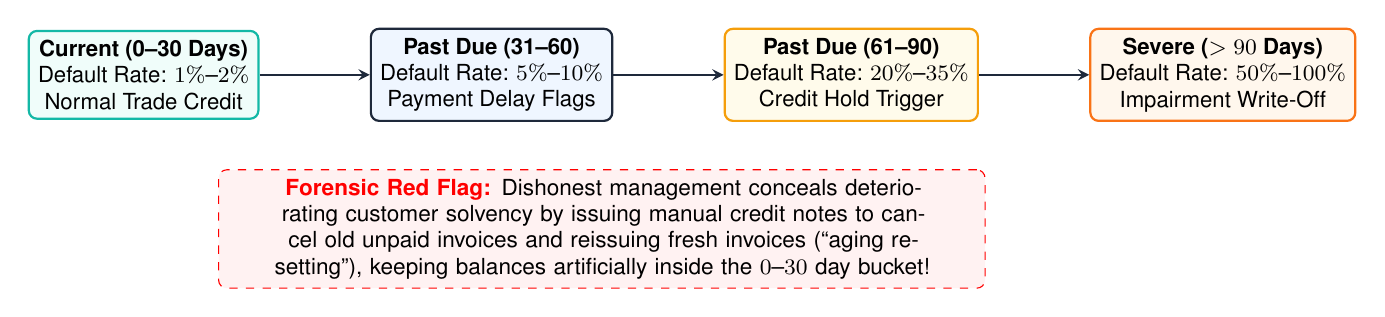
\begin{tikzpicture}[
    font=\sffamily\footnotesize,
    node distance=1.1cm and 1.4cm,
    step1/.style={rectangle, draw=tealborder, fill=tealbg, thick, rounded corners=3pt, minimum width=2.8cm, minimum height=1.1cm, align=center},
    step2/.style={rectangle, draw=primarydark, fill=primarylight, thick, rounded corners=3pt, minimum width=2.8cm, minimum height=1.1cm, align=center},
    step3/.style={rectangle, draw=amberborder, fill=amberbg, thick, rounded corners=3pt, minimum width=2.8cm, minimum height=1.1cm, align=center},
    step4/.style={rectangle, draw=coralborder, fill=coralbg, thick, rounded corners=3pt, minimum width=2.8cm, minimum height=1.1cm, align=center},
    arr/.style={->, >=stealth, thick, color=primarydark}
]

% Steps
\node[step1] (b1) {\textbf{Current (0--30 Days)}\\Default Rate: $1\%$--$2\%$\\Normal Trade Credit};
\node[step2, right=of b1] (b2) {\textbf{Past Due (31--60)}\\Default Rate: $5\%$--$10\%$\\Payment Delay Flags};
\node[step3, right=of b2] (b3) {\textbf{Past Due (61--90)}\\Default Rate: $20\%$--$35\%$\\Credit Hold Trigger};
\node[step4, right=of b3] (b4) {\textbf{Severe ($>90$ Days)}\\Default Rate: $50\%$--$100\%$\\Impairment Write-Off};

% Connectors
\draw[arr] (b1) -- (b2);
\draw[arr] (b2) -- (b3);
\draw[arr] (b3) -- (b4);

% Forensic Callout
\node[draw=red, dashed, fill=red!5, rounded corners=3pt, below=0.6cm of b2, xshift=1.4cm, text width=9.5cm, align=center] {
    \textcolor{red}{\textbf{Forensic Red Flag:}} Dishonest management conceals deteriorating customer solvency by issuing manual credit notes to cancel old unpaid invoices and reissuing fresh invoices (``aging resetting''), keeping balances artificially inside the $0$--$30$ day bucket!
};

\end{tikzpicture}
\caption{Accounts Receivable Aging Transition and Provisioning Escalation.}
\label{fig:ar_aging_ladder}
\end{figure}

% ----------------------------------------------------------------------
% PART 4: DEEP INTUITION & CONCEPTUAL DERIVATIONS
% ----------------------------------------------------------------------
\section{Deep Intuition \& Conceptual Derivations}

\subsection{The Masking Effect in Parametric Z-Score Audits}
Why does a standard $Z$-score fail in forensic fraud detection?
Suppose an enterprise ledger contains $1{,}000$ routine supplier payments averaging Rs.~$10{,}000$ with standard deviation $s = 2{,}000$. An embezzling controller introduces a massive single fraudulent payment of Rs.~$5{,}00{,}00{,}000$ (Rs.~$5$ Crores):
\begin{align*}
\bar{x}_{\text{new}} &\approx \frac{1000 \times 10{,}000 + 50{,}000{,}000}{1001} \approx \text{Rs.~} 59{,}940 \\
s_{\text{new}} &\approx \sqrt{\frac{1}{1000} \left(1000 \times (10{,}000 - 59{,}940)^2 + (50{,}000{,}000 - 59{,}940)^2\right)} \approx \text{Rs.~} 15{,}79{,}000
\end{align*}
Now, evaluate another suspicious payment of Rs.~$20{,}00{,}000$ (Rs.~$20$ Lakhs):
\begin{equation}
Z_i = \frac{2{,}000{,}000 - 59{,}940}{1{,}579{,}000} \approx 1.23
\end{equation}
A payment $200\times$ larger than normal operations yields a $Z$-score of only $1.23$, completely escaping detection because the massive Rs.~$5$ Crore transaction single-handedly inflated the sample standard deviation by $800\times$! This is known in robust statistics as the \textbf{masking effect}. 

Under the Modified $Z$-score:
\begin{align*}
\tilde{x} &= 10{,}000, \quad MAD = 1{,}349 \\
M_i &= \frac{0.6745 \times (2{,}000{,}000 - 10{,}000)}{1{,}349} \approx 995.2 \gg 3.5 \implies \text{\textcolor{red}{\textbf{Instantly Flagged!}}}
\end{align*}
The Median Absolute Deviation remains impervious to the extreme value (breakdown point of $50\%$).

% ----------------------------------------------------------------------
% PART 5: EXPLICIT GOTCHAS & DIAGNOSTIC MISCONCEPTIONS
% ----------------------------------------------------------------------
\section{Explicit Gotchas \& Diagnostic Misconceptions}

\begin{trapbox}{Gotcha 1: Conflating IRR with Actual Project Return}
\textbf{The Trap:} Assuming that an approved capital project with an $IRR$ of $35\%$ will compound the firm's invested capital at $35\%$ over its lifetime.\\
\textbf{Forensic Reality:} The mathematical formulation of $IRR$ inherently assumes that all intermediate project cash inflows can be reinvested at the $IRR$ itself ($35\%$), which is commercially unrealistic. The Modified Internal Rate of Return ($MIRR$), which reinvests inflows at the realistic Weighted Average Cost of Capital ($WACC$), provides the true economic yield.
\end{trapbox}

\begin{trapbox}{Gotcha 2: The Parametric Z-Score Breakdown in Skewed Financial Data}
\textbf{The Trap:} Applying Gaussian $\mu \pm 3\sigma$ filters to procurement payment ledgers and concluding that transactions below $3\sigma$ are normal.\\
\textbf{Forensic Reality:} Commercial transaction ledgers follow heavy-tailed distributions (log-normal or Pareto power-laws). In heavy-tailed data, extreme outliers distort both $\bar{x}$ and $\sigma$, causing severe masking where secondary fraudulent payments hide in plain sight.
\end{trapbox}

\begin{trapbox}{Gotcha 3: Neglecting the Low-Value Fraud Tail in Pareto Stratification}
\textbf{The Trap:} Auditing only the top $20\%$ of high-value disbursements under the Pareto 80/20 rule, assuming the remaining $80\%$ is immaterial.\\
\textbf{Forensic Reality:} Fraudsters are acutely aware of internal audit sampling thresholds. In procurement embezzlement, corrupt employees repeatedly submit thousands of low-value fake invoices (e.g., Rs.~$4{,}950$ to avoid a Rs.~$5{,}000$ voucher signoff rule). Auditing only top-tier transactions misses structuring and smurfing schemes entirely.
\end{trapbox}

\begin{trapbox}{Gotcha 4: Reversing Aging Provisions to Manufacture Paper Profits}
\textbf{The Trap:} Believing that changes in the bad debt provision matrix only reflect improved customer creditworthiness.\\
\textbf{Forensic Reality:} Dishonest management routinely reduces provision percentages on aged buckets (e.g., cutting the $>90$ days allowance from $50\%$ to $15\%$) during earnings slumps. This artificial adjustment reduces current-period bad debt expense, inflating reported Net Income without a single rupee of cash collection.
\end{trapbox}

% ----------------------------------------------------------------------
% PART 6: COMPARATIVE SYNTHESIS & SUMMARY TABLE
% ----------------------------------------------------------------------
\section{Comparative Synthesis \& Summary Table}

Table~\ref{tab:comparison_outliers} compares the statistical properties, breakdown bounds, and forensic suitability of parametric, non-parametric, and robust outlier detection algorithms.

\begin{table}[htbp]
\centering
\small
\begin{tabularx}{\textwidth}{lXXX}
\toprule
\textbf{Dimension} & \textbf{Parametric $Z$-Score} & \textbf{Tukey Boxplot (IQR)} & \textbf{Modified $Z$-Score (MAD)} \\
\midrule
\textbf{Distribution Assumption} & Strict Gaussian (Normal) distribution required. & Distribution-free; semi-parametric rank ordering. & Assumes underlying symmetric distribution around median. \\
\addlinespace
\textbf{Breakdown Point} & $0\%$ (a single extreme outlier can distort $\bar{x}$ and $s$). & $25\%$ (requires $>25\%$ contamination to corrupt quartiles). & $50\%$ (highest possible resistance to contamination). \\
\addlinespace
\textbf{Vulnerability to Masking} & Severe: high-value fraud inflates $s$, masking other anomalies. & Low: inner/outer fences remain stable under extreme spikes. & Minimal: median and MAD are completely robust to extreme tails. \\
\addlinespace
\textbf{Detection Threshold} & $|Z_i| > 3.0$ standard deviations. & $x_i > Q_3 + 1.5 \cdot IQR$ (outlier); $> Q_3 + 3.0 \cdot IQR$ (extreme). & $|M_i| > 3.5$ modified standard score. \\
\addlinespace
\textbf{Primary Audit Application} & Controlled manufacturing physical tolerances; standardized fees. & Accounts Receivable invoice aging; travel expense distributions. & Procurement journal audits; vendor payment amounts; wire transfers. \\
\bottomrule
\end{tabularx}
\caption{Comparative Matrix of Statistical Outlier Detection Frameworks in Financial Forensics.}
\label{tab:comparison_outliers}
\end{table}

% ----------------------------------------------------------------------
% PART 7: PYTHON / SCIENTIFIC COMPUTING LAB
% ----------------------------------------------------------------------
\section{Python / Scientific Computing Lab: Automated AR Aging \& Robust Outlier Detection}

Listing~\ref{lst:aging_outlier_engine} provides a complete, production-ready Python program that constructs accounts receivable aging schedules, calculates expected credit loss provisions, and executes robust Modified $Z$-score outlier filtering.

\begin{lstlisting}[language=Python, caption={Automated Invoice Aging \& Robust Outlier Detection in Python}, label={lst:aging_outlier_engine}]
import pandas as pd
import numpy as np

def audit_accounts_receivable(invoices_df: pd.DataFrame, as_of_date: str = '2025-03-31') -> dict:
    """
    Constructs an Accounts Receivable Aging Schedule and performs 
    Modified Z-score outlier detection on outstanding invoice amounts.
    
    Parameters:
        invoices_df (pd.DataFrame): Columns ['inv_id', 'customer', 'inv_date', 'amount']
        as_of_date (str): Audit balance cut-off date ('YYYY-MM-DD')
        
    Returns:
        dict: Aging schedule table, provisioning summary, and flagged outliers.
    """
    df = invoices_df.copy()
    df['inv_date'] = pd.to_datetime(df['inv_date'])
    ref_date = pd.to_datetime(as_of_date)
    
    # 1. Compute Days Past Due
    df['days_outstanding'] = (ref_date - df['inv_date']).dt.days
    
    # 2. Stratify into Aging Buckets
    bins = [-np.inf, 30, 60, 90, np.inf]
    labels = ['0-30 Days', '31-60 Days', '61-90 Days', '>90 Days']
    df['aging_bucket'] = pd.cut(df['days_outstanding'], bins=bins, labels=labels)
    
    # 3. Provisioning Rates Matrix
    prov_rates = {'0-30 Days': 0.01, '31-60 Days': 0.05, '61-90 Days': 0.20, '>90 Days': 0.50}
    df['provision_rate'] = df['aging_bucket'].map(prov_rates).astype(float)
    df['required_provision'] = df['amount'] * df['provision_rate']
    
    # Aging Summary Table
    aging_summary = df.groupby('aging_bucket', observed=False).agg(
        invoice_count=('inv_id', 'count'),
        total_balance=('amount', 'sum'),
        total_provision=('required_provision', 'sum')
    ).reset_index()
    aging_summary['effective_provision%'] = (
        aging_summary['total_provision'] / aging_summary['total_balance'] * 100.0
    ).round(2)
    
    # 4. Robust Outlier Detection: Modified Z-Score
    med = df['amount'].median()
    mad = np.median(np.abs(df['amount'] - med))
    if mad == 0:
        mad = np.mean(np.abs(df['amount'] - med))  # Fallback to mean absolute deviation
        
    df['modified_z'] = 0.6745 * (df['amount'] - med) / mad
    outliers = df[df['modified_z'].abs() > 3.5].copy()
    
    return {
        'total_ar_balance': df['amount'].sum(),
        'total_provision_required': df['required_provision'].sum(),
        'aging_schedule': aging_summary,
        'outlier_count': len(outliers),
        'flagged_outliers': outliers[['inv_id', 'customer', 'amount', 'days_outstanding', 'modified_z']]
    }

# -------------------------------------------------------------
# Test Harness with Aging Lag & Embezzlement Outliers
# -------------------------------------------------------------
if __name__ == '__main__':
    data = [
        {'inv_id': 'INV-101', 'customer': 'Alpha Corp', 'inv_date': '2025-03-15', 'amount': 15000.0},
        {'inv_id': 'INV-102', 'customer': 'Beta Ltd', 'inv_date': '2025-02-20', 'amount': 18500.0},
        {'inv_id': 'INV-103', 'customer': 'Gamma Ind', 'inv_date': '2025-01-10', 'amount': 22000.0},
        {'inv_id': 'INV-104', 'customer': 'Delta Retail', 'inv_date': '2024-11-05', 'amount': 35000.0},
        {'inv_id': 'INV-105', 'customer': 'Epsilon Tech', 'inv_date': '2025-03-25', 'amount': 14200.0},
        {'inv_id': 'INV-106', 'customer': 'Shell Co X', 'inv_date': '2025-03-28', 'amount': 850000.0} # Outlier!
    ]
    df_inv = pd.DataFrame(data)
    audit = audit_accounts_receivable(df_inv, as_of_date='2025-03-31')
    
    print(f"Total AR Outstanding: Rs. {audit['total_ar_balance']:,.2f}")
    print(f"Total Required Provision: Rs. {audit['total_provision_required']:,.2f}\n")
    print("Accounts Receivable Aging Schedule:")
    print(audit['aging_schedule'].to_string(index=False))
    print(f"\nFlagged Outliers (|Mod-Z| > 3.5): {audit['outlier_count']}")
    print(audit['flagged_outliers'].to_string(index=False))
\end{lstlisting}

% ----------------------------------------------------------------------
% PART 8: COMPREHENSIVE PRACTICE PROBLEMS
% ----------------------------------------------------------------------
\section{Comprehensive Practice Problems}
\textit{Complete mathematical derivations and diagnostic MCQ distractor rationales are located in the Appendix.}

\subsection*{Part A: Analytical \& Computational Problems}

\begin{enumerate}[label=\textbf{P6.\arabic*}]
    \item \textbf{Capital Budgeting Valuation \& Hurdle Rate Arbitrage:}\\
    An infrastructure developer is evaluating an industrial solar generation plant requiring an initial capital expenditure of Rs.~$100$ Crores at $t = 0$. Expected future net cash flows are:
    \begin{itemize}
        \item Year 1: Rs.~$25$ Crores, Year 2: Rs.~$35$ Crores, Year 3: Rs.~$40$ Crores, Year 4: Rs.~$45$ Crores.
    \end{itemize}
    \begin{enumerate}[label=(\alph*)]
        \item Compute the project's Net Present Value ($NPV$) assuming an enterprise cost of capital $k = 10\%$.
        \item State the decision rule for $NPV$ and determine whether the investment should be approved.
        \item If management artificially depresses the hurdle rate to $k = 6\%$ to push through a favored project, quantify the resulting artificial expansion in reported $NPV$.
    \end{enumerate}

    \item \textbf{Accounts Receivable Aging Schedule \& Provisioning Forensics:}\\
    At the close of the financial year, a logistics enterprise presents the following gross accounts receivable balances across aging brackets:
    \begin{center}
    \begin{tabular}{lrr}
    \toprule
    \textbf{Aging Bracket} & \textbf{Gross Receivables} & \textbf{Historical Default Rate} \\
    \midrule
    $0$--$30$ Days & Rs.~$50{,}00{,}000$ & $1.5\%$ \\
    $31$--$60$ Days & Rs.~$20{,}00{,}000$ & $6.0\%$ \\
    $61$--$90$ Days & Rs.~$12{,}00{,}000$ & $25.0\%$ \\
    $>90$ Days & Rs.~$8{,}00{,}000$ & $60.0\%$ \\
    \bottomrule
    \end{tabular}
    \end{center}
    \begin{enumerate}[label=(\alph*)]
        \item Calculate the total expected credit loss allowance required on the balance sheet.
        \item To meet an earnings benchmark, the CFO reclassifies Rs.~$6{,}00{,}000$ of receivables from the $>90$ Days bucket into the $0$--$30$ Days bucket by issuing replacement invoices. Compute the fraudulent reduction in bad debt expense and the percentage overstatement of pre-tax profit.
    \end{enumerate}

    \item \textbf{The Masking Effect in Forensic Outlier Detection:}\\
    A transaction ledger contains $n = 5$ vendor disbursements (in Rs.~Thousands): $[10, 12, 11, 13, 500]$.
    \begin{enumerate}[label=(\alph*)]
        \item Compute the sample mean $\bar{x}$ and sample standard deviation $s$.
        \item Compute the standard $Z$-score for the value $x = 13$.
        \item Compute the sample median $\tilde{x}$ and the Median Absolute Deviation ($MAD$).
        \item Compute the Modified $Z$-score $M_i$ for $x = 13$ and $x = 500$. Demonstrate why the Modified $Z$-score avoids the masking effect.
    \end{enumerate}

    \item \textbf{Tukey Interquartile Range (IQR) Non-Parametric Boundaries:}\\
    An auditor reviews the following ordered sample of monthly procurement office supply claims (in Rs.):
    \begin{equation*}
    [1200, 1400, 1500, 1650, 1800, 1950, 2100, 2300, 2800, 3100, 4500, 9800]
    \end{equation*}
    \begin{enumerate}[label=(\alph*)]
        \item Determine the first quartile ($Q_1$), median ($Q_2$), third quartile ($Q_3$), and $IQR$.
        \item Calculate the inner fences $[Q_1 - 1.5 \cdot IQR, Q_3 + 1.5 \cdot IQR]$ and outer fences $[Q_1 - 3.0 \cdot IQR, Q_3 + 3.0 \cdot IQR]$.
        \item Identify which claims qualify as mild outliers and which qualify as extreme outliers.
    \end{enumerate}

    \item \textbf{Pareto 80/20 Stratification \& Smurfing Audit Design:}\\
    A commercial bank processes $100{,}000$ international payments totaling Rs.~$500$ Crores annually. Explain how an investigative auditor should stratify this dataset using the Pareto principle to inspect both high-value concentration risks and structured smurfing schemes.
\end{enumerate}

\subsection*{Part B: Diagnostic Multiple-Choice Questions}

\begin{enumerate}[label=\textbf{MCQ 6.\arabic*}]
    \item Why is the Modified $Z$-score utilizing Median Absolute Deviation ($MAD$) preferred over the classical Gaussian $Z$-score when auditing commercial transaction ledgers for fraudulent disbursements?
    \begin{enumerate}[label=(\alph*)]
        \item The Gaussian $Z$-score can only be calculated for datasets with fewer than $30$ observations.
        \item Extreme fraudulent payments dramatically inflate both the sample mean and standard deviation, artificially reducing the calculated $Z$-scores of secondary fraudulent transactions (the masking effect).
        \item The Modified $Z$-score guarantees that the sum of all transaction amounts equals zero.
        \item Microsoft Excel is incapable of computing standard deviations on financial columns.
    \end{enumerate}

    \item Under the International Financial Reporting Standard (IFRS 9) expected credit loss framework, an enterprise discovers that a major customer's credit rating was downgraded from investment grade to sub-prime, and invoices have aged past $90$ days. What accounting entry is mandatory?
    \begin{enumerate}[label=(\alph*)]
        \item Derecognize the customer's accounts receivable and book a direct charge to Share Capital.
        \item Transfer the receivable balance into Intangible Goodwill.
        \item Recognize a lifetime expected credit loss allowance through a debit to Impairment Loss (Profit \& Loss) and a credit to Allowance for Doubtful Accounts (Contra-Asset).
        \item Defer recognizing any loss until the customer formally files for bankruptcy liquidation in court.
    \end{enumerate}
\end{enumerate}

\chapter{Advanced Corporate Finance \& the Financial Transaction Lifecycle}

\begin{tcolorbox}[colback=primarylight, colframe=primarydark, title={\textbf{What You Will Learn in this Chapter}}]
\begin{itemize}
    \item Cost of capital estimation: Weighted Average Cost of Capital (WACC) and the CAPM equation
    \item Operating vs.~Financial leverage and bankruptcy vulnerability (Altman $Z$-Score)
    \item The 5-stage Financial Transaction Lifecycle: Initiation, Authentication, Authorization, Clearing, and Settlement
    \item Architecture of global payment networks: Card Four-Party Model, SWIFT messaging, and UPI/Instant Rails
    \item Intercept touchpoints: Account Takeover (ATO), Authorized Push Payment (APP) fraud, and chargeback abuse
    \item State-machine Python simulation of financial transaction settlement and risk interception
\end{itemize}
\end{tcolorbox}

\section{Cost of Capital and Financial Risk}

An enterprise's \index{cost of capital}\textbf{Cost of Capital} represents the minimum expected return required by capital providers (debt holders and equity investors) to commit their funds to the firm.

\begin{definitionbox}{Weighted Average Cost of Capital (WACC)}
\index{WACC}
\begin{equation}
\text{WACC} = \left(\frac{E}{V}\right) \cdot r_e + \left(\frac{D}{V}\right) \cdot r_d \cdot (1 - T_c)
\end{equation}
where $E$ is market value of equity, $D$ is market value of debt, $V = E + D$, $r_d$ is before-tax cost of debt, $T_c$ is corporate marginal tax rate, and $r_e$ is cost of equity derived via the Capital Asset Pricing Model (CAPM):
\begin{equation}
r_e = R_f + \beta_e \cdot (E(R_m) - R_f)
\end{equation}
\end{definitionbox}

\begin{videocard}{IITM BS Lecture: Basics of Corporate Finance -- Part 5}{https://www.youtube.com/watch?v=P4WJgd6m91w}
Cost of debt, market yield vs.~coupon rate, and tax-shield advantages of corporate borrowing.
\end{videocard}

\begin{videocard}{IITM BS Lecture: Basics of Corporate Finance -- Part 6}{https://www.youtube.com/watch?v=EFqt4mvTGUM}
Equity valuation fundamentals, Gordon Growth model, and cost of equity derivation.
\end{videocard}

\begin{videocard}{IITM BS Lecture: Basics of Corporate Finance -- Part 7}{https://www.youtube.com/watch?v=oeHGl88x2dY}
Synthesizing capital structure optimization, financial leverage risks, and bankruptcy boundaries.
\end{videocard}

\section{Altman $Z$-Score for Distress and Solvency Forensics}

Developed by Professor Edward Altman in 1968, the \index{Altman Z-Score}\textbf{Altman $Z$-Score} is a multivariate statistical formula predicting the probability that an enterprise will enter bankruptcy within two years:
\begin{equation}
Z = 1.2 X_1 + 1.4 X_2 + 3.3 X_3 + 0.6 X_4 + 0.999 X_5
\end{equation}
where $X_1 = \frac{\text{Working Capital}}{\text{Total Assets}}$, $X_2 = \frac{\text{Retained Earnings}}{\text{Total Assets}}$, $X_3 = \frac{\text{EBIT}}{\text{Total Assets}}$, $X_4 = \frac{\text{Market Equity}}{\text{Total Liabilities}}$, and $X_5 = \frac{\text{Sales}}{\text{Total Assets}}$.

\begin{theorembox}{Altman $Z$-Score Decision Zones}
\begin{itemize}
    \item $Z > 2.99$: \textbf{Safe Zone} (Low probability of insolvency).
    \item $1.81 \le Z \le 2.99$: \textbf{Grey Zone} (Moderate distress; high scrutiny recommended).
    \item $Z < 1.81$: \textbf{Distress Zone} (High probability of default/insolvency).
\end{itemize}
\end{theorembox}

\section{The Five-Stage Financial Transaction Lifecycle}

Every electronic financial transaction migrates across five distinct operational phases:

\begin{figure}[htbp]
\centering
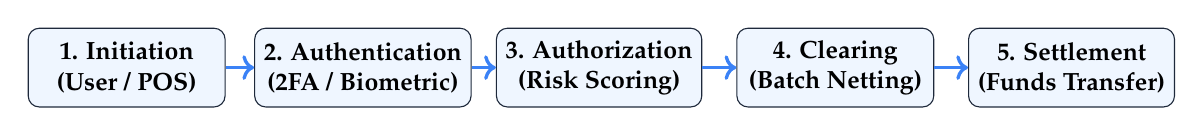
\begin{tikzpicture}[
  node distance=2.2cm,
  stage/.style={rectangle, draw=primarydark, fill=primarylight, rounded corners, minimum width=2.5cm, minimum height=1cm, font=\small\bfseries, align=center}
]
\node[stage] (init) {1. Initiation\\(User / POS)};
\node[stage, right of=init, xshift=0.8cm] (authn) {2. Authentication\\(2FA / Biometric)};
\node[stage, right of=authn, xshift=0.8cm] (authz) {3. Authorization\\(Risk Scoring)};
\node[stage, right of=authz, xshift=0.8cm] (clear) {4. Clearing\\(Batch Netting)};
\node[stage, right of=clear, xshift=0.8cm] (settle) {5. Settlement\\(Funds Transfer)};

\draw[->, very thick, primaryborder] (init) -- (authn);
\draw[->, very thick, primaryborder] (authn) -- (authz);
\draw[->, very thick, primaryborder] (authz) -- (clear);
\draw[->, very thick, primaryborder] (clear) -- (settle);
\end{tikzpicture}
\caption{The Five Core Stages of the Electronic Payment Lifecycle.}
\end{figure}

\begin{definitionbox}{Lifecycle Phases}
\index{Authentication}\index{Authorization}\index{Clearing}\index{Settlement}
\begin{enumerate}
    \item \textbf{Initiation:} The payer instructs their financial intermediary (or merchant POS) to transfer value.
    \item \textbf{Authentication:} Verification of the payer's legal identity via knowledge factors (PIN/password), possession factors (OTP/token), or inherence factors (fingerprint/FaceID).
    \item \textbf{Authorization:} Real-time risk verification by the issuing bank confirming account solvency, fraud risk score, and transaction limit adherence.
    \item \textbf{Clearing:} Exchange of payment instructions and fee calculation between issuing and acquiring institutions (often in deferred net settlement batches).
    \item \textbf{Settlement:} Irrevocable, final transfer of actual central bank reserves or interbank funds fulfilling the payment obligation.
\end{enumerate}
\end{definitionbox}

\begin{intuitionbox}{The Vulnerability Window Between Authorization and Settlement}
In credit card networks, \textit{Authorization} occurs in 200 milliseconds at the cash register, but \textit{Settlement} typically takes 24 to 48 hours. This structural time delay creates a vulnerability window exploited by fraudsters. In ``bust-out'' fraud, an identity thief runs up charges across multiple merchants simultaneously before the first transaction settles or alerts the cardholder.
\end{intuitionbox}

\begin{examplebox}{Historical Case Study: Wirecard AG Payment Lifecycle Fabrication (2020)}
\index{Wirecard Scandal}
German FinTech giant Wirecard AG collapsed into insolvency in June 2020 after auditors discovered that $€1.9\text{ Billion}$ in cash reserves did not exist:
\begin{itemize}
    \item \textbf{The Fraudulent Scheme:} Wirecard claimed to process billions in high-risk online payments across Asia through third-party acquiring partners (TPAs). Wirecard recognized massive revenues from these TPAs, claiming the cash proceeds were held in fiduciary escrow accounts at two major Philippine banks.
    \item \textbf{Payment Rail Manipulation:} In reality, the TPA transaction volumes were fabricated. When auditors attempted to verify the balances directly with the Philippine banks, the banks confirmed that Wirecard held no accounts and that the confirmation letters provided by management were forged.
    \item \textbf{Forensic Takeaway:} In digital payment forensics, relying on internal company ledger records without independent, cryptographically authenticated SWIFT confirmations directly from counterparty financial clearinghouses is fatal.
\end{itemize}
\end{examplebox}

\section{Data Science Relevance: Transaction State-Machine Simulation}

\begin{lstlisting}[caption={Financial Transaction Lifecycle \& Fraud Interception Simulation in Python}]
from enum import Enum
import random
import time

class TxnStatus(Enum):
    INITIATED = "INITIATED"
    AUTHENTICATED = "AUTHENTICATED"
    AUTHORIZED = "AUTHORIZED"
    DECLINED = "DECLINED"
    CLEARED = "CLEARED"
    SETTLED = "SETTLED"

class TransactionLifecycleEngine:
    def __init__(self, risk_threshold: float = 0.75):
        self.risk_threshold = risk_threshold

    def evaluate_risk(self, amount: float, velocity_1h: int, is_foreign: bool) -> float:
        """Heuristic risk score: Returns probability between 0 and 1."""
        score = 0.05
        if amount > 50000.0:
            score += 0.40
        if velocity_1h > 5:
            score += 0.35
        if is_foreign:
            score += 0.20
        return min(score, 0.99)

    def process_payment(self, txn_id: str, amount: float, velocity: int, foreign: bool) -> dict:
        log = {"txn_id": txn_id, "amount": amount, "history": []}
        
        # Stage 1 & 2: Initiation & Authentication
        log["history"].append(TxnStatus.INITIATED.value)
        log["history"].append(TxnStatus.AUTHENTICATED.value)
        
        # Stage 3: Real-Time Risk Authorization
        risk_score = self.evaluate_risk(amount, velocity, foreign)
        log["risk_score"] = round(risk_score, 3)
        
        if risk_score > self.risk_threshold:
            log["history"].append(TxnStatus.DECLINED.value)
            log["final_status"] = TxnStatus.DECLINED.value
            return log
        
        log["history"].append(TxnStatus.AUTHORIZED.value)
        
        # Stage 4 & 5: Clearing and Settlement
        log["history"].append(TxnStatus.CLEARED.value)
        log["history"].append(TxnStatus.SETTLED.value)
        log["final_status"] = TxnStatus.SETTLED.value
        return log

engine = TransactionLifecycleEngine(risk_threshold=0.70)
# Normal transaction
print(engine.process_payment("TXN_001", amount=1200.0, velocity=1, foreign=False))
# High risk transaction intercepted
print(engine.process_payment("TXN_002", amount=85000.0, velocity=7, foreign=True))
\end{lstlisting}

\section{Anti-Money Laundering (AML) \& The Financial Crime Lifecycle}

Money laundering is the illegal process of making large amounts of money generated by criminal activity (such as drug trafficking, corruption, or tax evasion) appear to have originated from a legitimate source.

\begin{theorembox}{The Three Stages of Money Laundering}
\index{Money Laundering}\index{Placement}\index{Layering}\index{Integration}
\begin{enumerate}
    \item \textbf{Placement:} The physical introduction of illicit bulk cash into the formal financial system.
    \begin{itemize}
        \item \textit{Smurfing / Structuring:} Breaking large cash sums into small transactions below mandatory statutory reporting thresholds (e.g., depositing Rs.~49,000 to bypass PAN card recording or below $\$10,000$ to evade FinCEN Currency Transaction Reports).
        \item \textit{Cash-Intensive Fronts:} Laundering cash through retail establishments (casinos, car washes, restaurants).
    \end{itemize}
    \item \textbf{Layering:} Obscuring the audit trail through complex, multi-layered financial transactions across international jurisdictions.
    \begin{itemize}
        \item Rapid wire transfers across nested offshore shell companies.
        \item \textbf{Trade-Based Money Laundering (TBML):} Over-invoicing or under-invoicing cross-border goods shipments to covertly shift value.
        \item \textbf{Hawala / Informal Value Transfer Systems (IVTS):} Trust-based settlement without physical currency border crossings.
    \end{itemize}
    \item \textbf{Integration:} Re-entering cleaned funds into the legitimate economy through investments in luxury real estate, securities, commercial ventures, or art.
\end{enumerate}
\end{theorembox}

\begin{theorembox}{RBI Master Directions: Early Warning Signals (EWS) \& Red Flagged Accounts (RFA)}
\index{Early Warning Signals}\index{Red Flagged Accounts}
Under Reserve Bank of India (RBI) guidelines, scheduled commercial banks must monitor a portfolio of \textbf{42 Early Warning Signals (EWS)} to identify potential loan fraud before default:
\begin{itemize}
    \item \textbf{Red Flagged Account (RFA):} An account where suspicion of fraudulent activity is triggered by EWS thresholds. An RFA must be investigated via forensic audit within 6 months.
    \item \textbf{Mandatory Reporting:} Confirmed frauds must be immediately reported to the Central Repository of Information on Large Credits (CRILC) and filed as a \textbf{Suspicious Transaction Report (STR)} with the Financial Intelligence Unit (FIU-IND).
\end{itemize}
\end{theorembox}

\section*{Supplementary Lecture Videos}
\begin{itemize}
    \item \href{https://www.youtube.com/watch?v=P4WJgd6m91w}{W7\_L1: Basics of Corporate Finance -- Part 5 (Cost of Debt \& Tax Shields)}
    \item \href{https://www.youtube.com/watch?v=EFqt4mvTGUM}{W7\_L2: Basics of Corporate Finance -- Part 6 (Equity Valuation \& CAPM)}
    \item \href{https://www.youtube.com/watch?v=oeHGl88x2dY}{W7\_L3: Basics of Corporate Finance -- Part 7 (Capital Structure Optimization)}
    \item \href{https://www.youtube.com/watch?v=OO0VpntKrPg}{W8\_L1: Introduction to Financial Transaction Lifecycle}
\end{itemize}

\newpage
\section{Practice Exercises}
\textit{Detailed step-by-step solutions are available in the Appendix.}

\begin{enumerate}
    \item Delta Industrial Corp.~has an equity market capitalization of Rs.~600 Crores and total outstanding debt with a market value of Rs.~400 Crores. The company's equity beta is $\beta_e = 1.25$, the risk-free rate $R_f = 6.5\%$, and the expected market return $E(R_m) = 14.5\%$. The firm pays an average pre-tax borrowing cost of $9.0\%$ on its debt and faces a marginal corporate tax rate of $25\%$. Calculate the firm's Weighted Average Cost of Capital (WACC).
    
    \item Compute the Altman $Z$-Score for Zenith Manufacturing given the following metrics: Working Capital = Rs.~2,00,000; Total Assets = Rs.~10,00,000; Retained Earnings = Rs.~1,50,000; EBIT = Rs.~1,20,000; Market Value of Equity = Rs.~4,00,000; Total Liabilities = Rs.~6,00,000; and Total Sales = Rs.~9,00,000. Classify Zenith into its appropriate Altman risk zone.
    
    \item Distinguish between Gross Settlement (as in RTGS) and Net Settlement (as in ACH or batch clearing) systems. Detail how systemic settlement risk manifests if an participating bank defaults before net clearing commitments are settled.
    
    \item Explain the mechanics of an Authorized Push Payment (APP) fraud scheme. Why do traditional two-factor authentication (2FA) controls fail to prevent APP fraud when an adversary uses social engineering to impersonate an enforcement officer?
    
    \item In the traditional Four-Party Card Payment Model, identify the four primary participating entities. At which exact operational interface is interchange fee calculated and deducted?
\end{enumerate}

\chapter{Credit Risk, Probability of Default \& Reject Inferencing}

% ----------------------------------------------------------------------
% PART 1: EXECUTIVE ROADMAP & LEARNING OBJECTIVES
% ----------------------------------------------------------------------
\section{Executive Roadmap \& Learning Objectives}

Credit risk represents the largest single category of financial risk faced by commercial banking institutions, defined as the potential that a bank borrower or counterparty will fail to meet their obligations in accordance with agreed contractual terms. Under the international Basel regulatory accords, credit exposure is quantitatively managed through structural risk engines that estimate borrower default probabilities. In applied financial data science, credit modeling faces a severe foundational econometric challenge: \textbf{selection bias}. Because credit scoring models can only observe repayment performance on applicants who were previously accepted, unadjusted models suffer catastrophic bias unless corrected through rigorous reject inferencing.

\begin{tcolorbox}[colback=primarylight, colframe=primarydark, title={\textbf{Core Learning Competencies}}]
Upon mastering this chapter, students will be equipped to:
\begin{itemize}
    \item \textbf{Formulate the Basel Credit Loss Paradigm:} Calculate Expected Loss ($EL$) through Probability of Default ($PD$), Loss Given Default ($LGD$), and Exposure at Default ($EAD$).
    \item \textbf{Develop Logistic Default Scoring Models:} Transform continuous financial applicant features into calibrated log-odds and default probabilities via sigmoid logistic regression.
    \item \textbf{Execute Weight of Evidence (WoE) Feature Engineering:} Linearize complex monotonic credit variables and evaluate feature predictive power via Information Value ($IV$).
    \item \textbf{Correct for Selection Bias via Reject Inferencing:} Overcome the accepted-only sample distortion using Hard Cutoff, Augmentation, and Parceling techniques.
    \item \textbf{Validate Scoring Engine Discrimination:} Evaluate credit models using the Receiver Operating Characteristic Area Under the Curve (ROC-AUC), Gini coefficient, and Kolmogorov-Smirnov ($KS$) metric.
\end{itemize}
\end{tcolorbox}

\begin{table}[htbp]
\centering
\small
\begin{tabularx}{\textwidth}{llX}
\toprule
\textbf{Construct / Metric} & \textbf{Symbol} & \textbf{Mathematical Definition / Decision Rule} \\
\midrule
Expected Loss & $EL$ & $PD \times LGD \times EAD$ \\
Logistic Default Probability & $p(Y=1 \mid \mathbf{x})$ & $\sigma(\boldsymbol{\beta}^T \mathbf{x}) = \frac{1}{1 + e^{-(\beta_0 + \sum \beta_j x_j)}}$ \\
Log-Odds (Logit) & $\ln\left(\frac{p}{1-p}\right)$ & $\boldsymbol{\beta}^T \mathbf{x} = \beta_0 + \beta_1 x_1 + \dots + \beta_k x_k$ \\
Weight of Evidence & $\text{WoE}_i$ & $\ln\left(\frac{\% \text{Non-Defaults}_i}{\% \text{Defaults}_i}\right) = \ln\left(\frac{G_i / G_{\text{total}}}{B_i / B_{\text{total}}}\right)$ \\
Information Value & $IV$ & $\sum_{i=1}^k \left(\frac{G_i}{G_{\text{total}}} - \frac{B_i}{B_{\text{total}}}\right) \times \text{WoE}_i$ \\
Gini Coefficient & $\text{Gini}$ & $2 \cdot \text{AUC} - 1$ \\
Scorecard Scaling & $\text{Score}$ & $\text{Offset} + \text{Factor} \cdot \ln\left(\frac{1-p}{p}\right)$ \\
\bottomrule
\end{tabularx}
\caption{Mathematical Notation Guide for Credit Risk Modeling and Scorecard Engineering.}
\label{tab:w8_notation}
\end{table}

% ----------------------------------------------------------------------
% PART 2: MATHEMATICAL & COMPUTATIONAL FOUNDATIONS
% ----------------------------------------------------------------------
\section{Mathematical \& Computational Foundations}

\subsection{The Basel Expected Loss Framework}
Under Basel II and III Internal Ratings-Based (IRB) approaches, financial institutions calculate the statistical mean loss expected over a 1-year horizon:
\begin{equation}
EL = PD \times LGD \times EAD
\label{eq:basel_el}
\end{equation}
where:
\begin{itemize}
    \item $PD \in [0, 1]$ represents the 12-month probability that the borrower will experience a credit event (e.g., $90+$ days past due or bankruptcy).
    \item $LGD = 1 - \text{Recovery Rate}$ represents the percentage loss net of collateral liquidation and legal recovery expenses.
    \item $EAD$ is the gross monetary balance outstanding at the time of default, incorporating drawn balances plus a credit conversion factor ($CCF$) on undrawn committed credit lines.
\end{itemize}

\subsection{Logistic Regression Calibration for Probability of Default}
Borrower binary default status $Y \in \{0, 1\}$ (where $Y=1$ indicates default) is modeled conditioned on risk covariates $\mathbf{x} \in \mathbb{R}^k$:
\begin{equation}
\ln\left(\frac{p(\mathbf{x})}{1 - p(\mathbf{x})}\right) = \beta_0 + \sum_{j=1}^k \beta_j x_j \implies p(\mathbf{x}) = \frac{1}{1 + \exp\left(-\left(\beta_0 + \sum_{j=1}^k \beta_j x_j\right)\right)}
\label{eq:logistic_pd}
\end{equation}
Model parameters $\boldsymbol{\beta}$ are estimated by maximizing the Bernoulli log-likelihood over $N$ historical training applicants:
\begin{equation}
\ell(\boldsymbol{\beta}) = \sum_{i=1}^N \left[ y_i \ln(p(\mathbf{x}_i)) + (1 - y_i) \ln(1 - p(\mathbf{x}_i)) \right]
\label{eq:log_likelihood}
\end{equation}

\subsection{Weight of Evidence (WoE) and Information Value (IV)}
In regulatory credit scoring, raw numerical continuous variables (e.g., Debt-to-Income, Age, Account Balance) are partitioned into $k$ discrete bins. For bin $i$:
\begin{equation}
\text{WoE}_i = \ln\left(\frac{\text{Good}_i / \text{Good}_{\text{total}}}{\text{Bad}_i / \text{Bad}_{\text{total}}}\right)
\label{eq:woe_formula}
\end{equation}
Information Value ($IV$) aggregates the divergence between Good and Bad distributions across all bins:
\begin{equation}
IV = \sum_{i=1}^k \left( \frac{\text{Good}_i}{\text{Good}_{\text{total}}} - \frac{\text{Bad}_i}{\text{Bad}_{\text{total}}} \right) \cdot \text{WoE}_i
\label{eq:iv_formula}
\end{equation}

\begin{theorembox}{Information Value Predictive Power Benchmarks}
\begin{itemize}
    \item $IV < 0.02$: \textbf{Unusable} for credit prediction; discard feature.
    \item $0.02 \le IV < 0.10$: \textbf{Weak Predictor}; marginal discriminatory power.
    \item $0.10 \le IV < 0.30$: \textbf{Medium Predictor}; standard predictive credit feature.
    \item $0.30 \le IV \le 0.50$: \textbf{Strong Predictor}; excellent standalone separation.
    \item $IV > 0.50$: \textbf{Suspicious / Potential Leakage}; likely includes post-default attributes.
\end{itemize}
\end{theorembox}

% ----------------------------------------------------------------------
% PART 3: VISUAL & GEOMETRIC INTUITION
% ----------------------------------------------------------------------
\section{Visual \& Geometric Intuition: The Sigmoid Decision Boundary}

Figure~\ref{fig:logistic_sigmoid} illustrates the transformation of a linear credit risk index ($\boldsymbol{\beta}^T \mathbf{x}$) into a bounded probability of default ($PD \in [0, 1]$), showing the decision cutoff threshold separating approvals from automated rejections.

\begin{figure}[htbp]
\centering
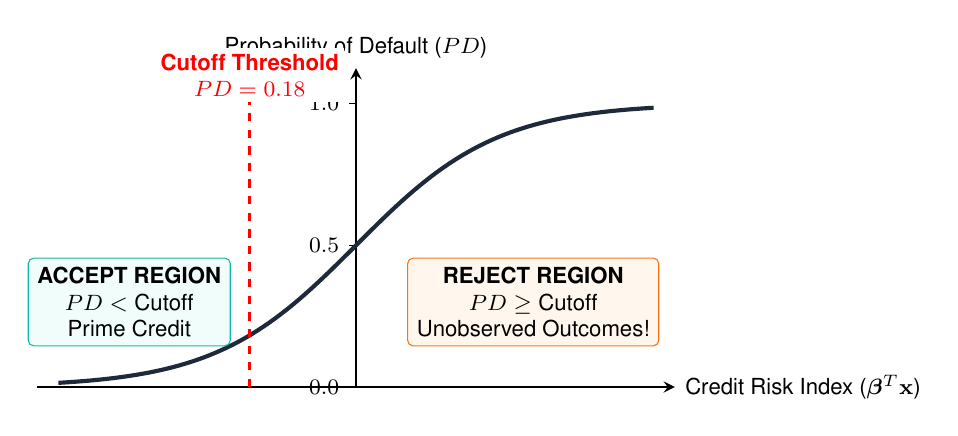
\begin{tikzpicture}[
    scale=0.9,
    font=\sffamily\footnotesize
]

% Axes
\draw[->, >=stealth, thick] (-4.5, 0) -- (4.5, 0) node[right] {Credit Risk Index ($\boldsymbol{\beta}^T \mathbf{x}$)};
\draw[->, >=stealth, thick] (0, 0) -- (0, 4.5) node[above] {Probability of Default ($PD$)};

% Ticks
\draw (0, 4) -- (-0.1, 4) node[left] {$1.0$};
\draw (0, 2) -- (-0.1, 2) node[left] {$0.5$};
\draw (0, 0) -- (-0.1, 0) node[left] {$0.0$};

% Sigmoid curve
\draw[line width=1.5pt, color=primarydark, domain=-4.2:4.2, samples=100] 
    plot (\x, {4 / (1 + exp(-\x))});

% Decision Threshold
\draw[dashed, line width=1.2pt, color=red] (-1.5, 0) -- (-1.5, 4.2);
\node[color=red, align=center, fill=white, inner sep=2pt] at (-1.5, 4.4) {\textbf{Cutoff Threshold}\\$PD = 0.18$};

% Regions
\node[draw=tealborder, fill=tealbg, rounded corners=2pt, align=center] at (-3.2, 1.2) {\textbf{ACCEPT REGION}\\$PD < \text{Cutoff}$\\Prime Credit};
\node[draw=coralborder, fill=coralbg, rounded corners=2pt, align=center] at (2.5, 1.2) {\textbf{REJECT REGION}\\$PD \ge \text{Cutoff}$\\Unobserved Outcomes!};

\end{tikzpicture}
\caption{The Logistic Sigmoid Default Calibration and the Selection Bias Boundary.}
\label{fig:logistic_sigmoid}
\end{figure}

% ----------------------------------------------------------------------
% PART 4: DEEP INTUITION & CONCEPTUAL DERIVATIONS
% ----------------------------------------------------------------------
\section{Deep Intuition \& Conceptual Derivations}

\subsection{The Econometric Problem of Selection Bias in Credit Forensics}
Credit scoring models encounter a fundamental missing-data challenge known as \index{selection bias}\textbf{selection bias}. The total applicant population arriving ``through-the-door'' ($\mathcal{P}_{\text{TTD}}$) is partitioned by the underwriting policy into:
\begin{equation}
\mathcal{P}_{\text{TTD}} = \mathcal{P}_{\text{Accepted}} \cup \mathcal{P}_{\text{Rejected}}
\end{equation}
For all applicants in $\mathcal{P}_{\text{Accepted}}$, the lender subsequently observes actual loan repayment or default ($Y \in \{0, 1\}$). However, for $\mathcal{P}_{\text{Rejected}}$, the enterprise never disburses funds; hence, their true default outcomes are permanently unobserved ($Y = \text{NaN}$).

If a data science team trains a default model exclusively on $\mathcal{P}_{\text{Accepted}}$:
\begin{equation}
p(Y=1 \mid \mathbf{x}, \text{Accepted}=1) \ne p(Y=1 \mid \mathbf{x}, \text{TTD})
\end{equation}
Because rejected applicants typically possess inferior credit characteristics, training only on accepted borrowers leads to severe underestimation of default probabilities when underwriting standards are loosened or expanded into new demographic segments.

\subsection{Reject Inferencing Methodologies}
To restore econometric validity across the entire through-the-door population, forensic modelers deploy three primary reject inferencing strategies:
\begin{enumerate}
    \item \textbf{Hard Cutoff Assignment:} Score all rejected applicants using the preliminary accepted-only model. Assign all rejects with score below a cutoff as Bad ($Y=1$), and the remainder as Good ($Y=0$). This artificially polarizes predictions.
    \item \textbf{Simple Augmentation (Re-weighting):} Retain only the accepted sample, but weight each accepted observation by the inverse probability of acceptance:
    \begin{equation}
    w_i = \frac{1}{P(\text{Accepted} \mid \mathbf{x}_i)}
    \end{equation}
    Accepted borrowers whose characteristics resemble rejected applicants receive higher sample weights.
    \item \textbf{Parceling (Proportional Re-assignment):} Partition the scored reject population into score bands. For each band, estimate the default rate by multiplying the accepted default rate by an empirical expansion factor ($2.0 \times$ to $3.5 \times$). Randomly allocate Bad labels to match this target default rate, merge with the accepted dataset, and re-estimate the final production scorecard.
\end{enumerate}

% ----------------------------------------------------------------------
% PART 5: EXPLICIT GOTCHAS & DIAGNOSTIC MISCONCEPTIONS
% ----------------------------------------------------------------------
\section{Explicit Gotchas \& Diagnostic Misconceptions}

\begin{trapbox}{Gotcha 1: Ignoring Reject Inferencing and Selection Bias}
\textbf{The Trap:} Training a credit risk model exclusively on historical accepted borrowers and assuming it will perform reliably across general population underwriting.\\
\textbf{Forensic Reality:} An accepted-only model never observes the delinquency behavior of sub-prime applicants who were previously rejected. When the bank launches an aggressive expansion campaign, the model severely under-predicts default rates, leading to catastrophic unexpected credit losses.
\end{trapbox}

\begin{trapbox}{Gotcha 2: The Linear Weighting Fallacy in Raw Ratio Scoring}
\textbf{The Trap:} Fitting a standard linear regression directly to raw financial ratios (e.g., Debt-to-Income or Current Ratio) without non-linear transformation.\\
\textbf{Forensic Reality:} The relationship between financial ratios and default probability is non-linear and non-monotonic. For example, zero credit utilization often carries higher risk than modest $15\%$ utilization. Transforming features into binned Weight of Evidence ($\text{WoE}$) establishes a strictly linear relationship with log-odds while gracefully handling outliers and missing values.
\end{trapbox}

\begin{trapbox}{Gotcha 3: Conflating Expected Loss with Regulatory Economic Capital}
\textbf{The Trap:} Assuming that a bank's capital reserves must equal its Expected Loss ($EL$).\\
\textbf{Forensic Reality:} Expected Loss is an anticipated recurring business cost, covered directly through credit margins and loan loss provisions (P\&L reserves). Equity capital (Tier-1 capital under Basel III) is held against \textbf{Unexpected Loss ($UL$)} at a $99.9\%$ confidence interval to protect depositors during severe economic crises.
\end{trapbox}

\begin{trapbox}{Gotcha 4: Overfitting on Suspiciously High Information Value}
\textbf{The Trap:} Celebrating a candidate feature that yields an Information Value $IV = 0.65$ as a revolutionary predictive discovery.\\
\textbf{Forensic Reality:} In commercial banking datasets, $IV > 0.50$ almost always signals target data leakage or temporal contamination. Variables such as ``Days Delinquent in Last 30 Days'' or ``Collection Call Count'' were populated after the borrower missed payments, creating artificial predictive illusion.
\end{trapbox}

% ----------------------------------------------------------------------
% PART 6: COMPARATIVE SYNTHESIS & SUMMARY TABLE
% ----------------------------------------------------------------------
\section{Comparative Synthesis \& Summary Table}

Table~\ref{tab:comparison_reject_inferencing} compares the four primary reject inferencing methodologies utilized across institutional banking environments.

\begin{table}[htbp]
\centering
\small
\begin{tabularx}{\textwidth}{lXXX}
\toprule
\textbf{Methodology} & \textbf{Core Statistical Mechanism} & \textbf{Bias Correction Efficacy} & \textbf{Regulatory Acceptability} \\
\midrule
\textbf{Hard Cutoff} & Assigns deterministic Good/Bad labels based on preliminary score cutoff. & Poor; artificially distorts score distributions and inflates separation. & Generally rejected by banking regulators (RBI, Federal Reserve, PRA). \\
\addlinespace
\textbf{Simple Augmentation} & Re-weights accepted observations by inverse probability of selection ($1/P_{\text{acc}}$). & Moderate; inflates variance if selection probabilities are near zero. & Acceptable under conservative weighting caps and stability testing. \\
\addlinespace
\textbf{Parceling} & Bins rejects and injects simulated defaults proportional to accepted risk multipliers ($2\times$--$3\times$). & High; preserves natural continuous score gradation and reflects known risk. & Gold standard in retail banking, mortgage underwriting, and auto finance. \\
\addlinespace
\textbf{Heckman Two-Stage (Bivariate Probit)} & Explicitly models selection equation and adds inverse Mills ratio to outcome equation. & Econometrically rigorous; requires valid instrumental variables. & Highly respected in econometric stress testing, but computationally complex. \\
\bottomrule
\end{tabularx}
\caption{Comparative Synthesis of Reject Inferencing Methodologies in Credit Risk Engineering.}
\label{tab:comparison_reject_inferencing}
\end{table}

% ----------------------------------------------------------------------
% PART 7: PYTHON / SCIENTIFIC COMPUTING LAB
% ----------------------------------------------------------------------
\section{Python / Scientific Computing Lab: Credit Scorecard Engineering Engine}

Listing~\ref{lst:credit_scorecard_engine} implements an automated credit risk pipeline that performs Weight of Evidence (WoE) transformation, evaluates Information Value (IV), trains a logistic default model, and computes ROC-AUC metrics.

\begin{lstlisting}[language=Python, caption={Credit Probability of Default \& WoE Pipeline in Python}, label={lst:credit_scorecard_engine}]
import numpy as np
import pandas as pd
from sklearn.linear_model import LogisticRegression
from sklearn.metrics import roc_auc_score

def compute_woe_iv(df: pd.DataFrame, feature: str, target: str, bins: int = 5) -> tuple:
    """
    Computes Weight of Evidence (WoE) and Information Value (IV) for a continuous feature.
    """
    df_temp = df[[feature, target]].copy()
    df_temp['bin'] = pd.qcut(df_temp[feature], q=bins, duplicates='drop')
    
    # Calculate Good (target=0) and Bad (target=1)
    stat = df_temp.groupby('bin', observed=False)[target].agg(
        total='count',
        bads='sum'
    ).reset_index()
    stat['goods'] = stat['total'] - stat['bads']
    
    total_goods = stat['goods'].sum()
    total_bads = stat['bads'].sum()
    
    # Prevent division by zero with Laplace smoothing
    stat['goods_dist'] = np.clip(stat['goods'] / total_goods, 1e-6, 1.0)
    stat['bads_dist'] = np.clip(stat['bads'] / total_bads, 1e-6, 1.0)
    
    # Compute WoE and IV
    stat['woe'] = np.log(stat['goods_dist'] / stat['bads_dist'])
    stat['iv_bin'] = (stat['goods_dist'] - stat['bads_dist']) * stat['woe']
    total_iv = stat['iv_bin'].sum()
    
    # Map WoE back to values
    woe_map = dict(zip(stat['bin'], stat['woe']))
    df_temp[f'{feature}_woe'] = df_temp['bin'].map(woe_map)
    
    return total_iv, stat[['bin', 'goods', 'bads', 'woe', 'iv_bin']], df_temp[f'{feature}_woe']

# -------------------------------------------------------------
# Test Harness with Credit Application Population
# -------------------------------------------------------------
if __name__ == '__main__':
    np.random.seed(42)
    n_samples = 2000
    
    # Feature 1: Debt-to-Income (DTI) ratio
    dti = np.random.uniform(0.1, 0.8, size=n_samples)
    # Feature 2: Credit Bureau Score (300 - 850)
    cibil = np.random.normal(loc=650, scale=80, size=n_samples).clip(300, 850)
    
    # Latent logit default probability
    z = -3.5 + 4.5 * dti - 0.006 * (cibil - 600)
    prob_default = 1.0 / (1.0 + np.exp(-z))
    default_status = np.random.binomial(n=1, p=prob_default)
    
    credit_df = pd.DataFrame({'dti': dti, 'cibil': cibil, 'default': default_status})
    
    # Evaluate WoE and IV for CIBIL
    cibil_iv, cibil_table, credit_df['cibil_woe'] = compute_woe_iv(credit_df, 'cibil', 'default')
    dti_iv, dti_table, credit_df['dti_woe'] = compute_woe_iv(credit_df, 'dti', 'default')
    
    print(f"Information Value (DTI): {dti_iv:.4f}")
    print(f"Information Value (CIBIL): {cibil_iv:.4f}\n")
    print("CIBIL WoE Binning Table:")
    print(cibil_table.to_string(index=False))
    
    # Train Logistic Regression on WoE features
    X = credit_df[['dti_woe', 'cibil_woe']]
    y = credit_df['default']
    clf = LogisticRegression()
    clf.fit(X, y)
    
    predicted_pd = clf.predict_proba(X)[:, 1]
    auc = roc_auc_score(y, predicted_pd)
    gini = 2 * auc - 1
    
    print(f"\nModel Discrimination Performance:")
    print(f"ROC-AUC: {auc:.4f} | Gini Coefficient: {gini:.4f}")
\end{lstlisting}

% ----------------------------------------------------------------------
% PART 8: COMPREHENSIVE PRACTICE PROBLEMS
% ----------------------------------------------------------------------
\section{Comprehensive Practice Problems}
\textit{Complete mathematical derivations and diagnostic MCQ distractor rationales are located in the Appendix.}

\subsection*{Part A: Analytical \& Computational Problems}

\begin{enumerate}[label=\textbf{P8.\arabic*}]
    \item \textbf{Basel Expected Loss Portfolio Calculation:}\\
    A commercial bank extends a corporate revolving working capital credit facility of Rs.~$50$ Crores to an industrial exporter. The bank's risk rating system assigns the following parameters:
    \begin{itemize}
        \item 12-month Probability of Default: $PD = 2.5\%$.
        \item Currently drawn principal balance: Rs.~$30$ Crores.
        \item Undrawn committed credit limit: Rs.~$20$ Crores, with a Credit Conversion Factor $CCF = 50\%$.
        \item The loan is partially secured by industrial real estate with an expected liquidation recovery rate of $40\%$ ($LGD = 60\%$).
    \end{itemize}
    \begin{enumerate}[label=(\alph*)]
        \item Compute the Exposure at Default ($EAD$).
        \item Calculate the 1-year Expected Loss ($EL$) in Rupees.
        \item If the credit rating degrades, pushing $PD$ to $6.0\%$ and increasing $LGD$ to $75\%$, calculate the required percentage increase in loan loss provisions.
    \end{enumerate}

    \item \textbf{Logistic Regression Logit to Probability Conversion:}\\
    A consumer credit default model calibrates default risk using the logit equation:
    \begin{equation*}
    z = \ln\left(\frac{p}{1-p}\right) = -2.80 + 2.40 \cdot \text{DTI} - 0.005 \cdot (\text{CIBIL} - 600) + 0.85 \cdot \text{Inquiries}
    \end{equation*}
    An applicant presents with a Debt-to-Income ratio $\text{DTI} = 0.45$, a bureau score $\text{CIBIL} = 680$, and $\text{Inquiries} = 2$.
    \begin{enumerate}[label=(\alph*)]
        \item Compute the log-odds value $z$.
        \item Calculate the applicant's calibrated Probability of Default ($PD$).
        \item If the bank's maximum allowable default risk threshold for loan approval is $PD \le 8.0\%$, state the underwriting decision.
    \end{enumerate}

    \item \textbf{Weight of Evidence (WoE) \& Information Value (IV) Derivation:}\\
    An analyst partitions $10{,}000$ retail applicants into three age brackets, observing the following Good ($Y=0$) and Bad ($Y=1$) distribution:
    \begin{center}
    \begin{tabular}{lrr}
    \toprule
    \textbf{Age Bracket} & \textbf{Good Borrowers} & \textbf{Bad Borrowers (Defaults)} \\
    \midrule
    $< 25$ Years & $1{,}600$ & $400$ \\
    $25$--$45$ Years & $5{,}400$ & $600$ \\
    $> 45$ Years & $2{,}000$ & $1000$ \\
    \midrule
    \textbf{Total} & \textbf{9,000} & \textbf{1,100} \\
    \bottomrule
    \end{tabular}
    \end{center}
    \begin{enumerate}[label=(\alph*)]
        \item Compute the percentage distribution of Goods and Bads for each age bucket.
        \item Calculate the Weight of Evidence ($\text{WoE}$) for each age bracket.
        \item Calculate the overall Information Value ($IV$) and evaluate its predictive strength.
    \end{enumerate}

    \item \textbf{Credit Scorecard Scaling and Points to Double the Odds:}\\
    A retail credit scoring department transforms log-odds into standard scorecard points using the affine transformation:
    \begin{equation*}
    \text{Score} = \text{Offset} + \text{Factor} \cdot \ln(\text{Odds}), \quad \text{where } \text{Odds} = \frac{1 - p}{p}
    \end{equation*}
    The scorecard is calibrated such that a borrower with $\text{Odds} = 50:1$ receives $600$ points, and the score doubles every time the odds double ($\text{PDO} = 20$ points).
    \begin{enumerate}[label=(\alph*)]
        \item Compute the scaling constants $\text{Factor}$ and $\text{Offset}$.
        \item Calculate the scorecard points for an applicant whose calibrated default probability is $p = 4.0\%$.
    \end{enumerate}

    \item \textbf{Reject Inferencing via the Parceling Technique:}\\
    Explain the mathematical steps required to implement reject inferencing via parceling. Detail how an accepted-only default rate is adjusted by an empirical expansion multiplier to re-label the rejected applicant pool.
\end{enumerate}

\subsection*{Part B: Diagnostic Multiple-Choice Questions}

\begin{enumerate}[label=\textbf{MCQ 8.\arabic*}]
    \item When developing institutional credit default models, what is the primary econometric risk of training scoring engines exclusively on historical accepted borrowers while omitting rejected applicants?
    \begin{enumerate}[label=(\alph*)]
        \item The model violates double-entry accounting invariants across balance sheet accounts.
        \item The model suffers from severe selection bias, resulting in systematically underestimating default risk when deployed across the broader, unselected applicant population.
        \item The model becomes computationally intractable because accepted borrowers have zero variance in credit scores.
        \item The model fails to satisfy Benford's Law leading-digit distribution.
    \end{enumerate}

    \item A credit risk data scientist computes an Information Value $IV = 0.62$ for a candidate variable named \texttt{days\_in\_collections\_last\_month}. How should a forensic model validator interpret this metric?
    \begin{enumerate}[label=(\alph*)]
        \item Approve the feature immediately because any $IV > 0.50$ represents industry gold-standard predictive power.
        \item Reject the feature because an $IV > 0.50$ strongly indicates target data leakage, since collection actions occur only after a credit default event has already taken place.
        \item Apply a logarithmic transformation to reduce the $IV$ below $0.10$.
        \item Re-scale the variable using the Altman $Z$-score formula.
    \end{enumerate}
\end{enumerate}

\chapter{Fraud Detection: Supervised \& Unsupervised Machine Learning}

% ----------------------------------------------------------------------
% PART 1: EXECUTIVE ROADMAP & LEARNING OBJECTIVES
% ----------------------------------------------------------------------
\section{Executive Roadmap \& Learning Objectives}

The exponential growth of real-time digital transaction volumes has rendered manual rule-based audit checks obsolete. Modern financial institutions process thousands of payment authorizations per second, requiring automated machine learning engines capable of identifying subtle fraud patterns within milliseconds. However, applying machine learning to financial fraud presents a unique set of foundational challenges: extreme class imbalance ($< 0.1\%$ positive incidence), asymmetric misclassification costs, and dynamic adversarial drift where fraudsters continuously alter their techniques.

\begin{tcolorbox}[colback=primarylight, colframe=primarydark, title={\textbf{Core Learning Competencies}}]
Upon mastering this chapter, students will be equipped to:
\begin{itemize}
    \item \textbf{Map Modern Financial Fraud Typologies:} Differentiate between synthetic identity theft, account takeover (ATO), and organized bust-out schemes.
    \item \textbf{Deconstruct the Accuracy Paradox:} Formulate cost-sensitive loss matrices and evaluate models using Precision-Recall Area Under the Curve (PR-AUC) rather than raw accuracy.
    \item \textbf{Engineer Resampling Strategies:} Apply Synthetic Minority Over-sampling Technique (SMOTE) and informed undersampling without inducing synthetic artifact contamination.
    \item \textbf{Deploy Supervised Gradient Boosters:} Train cost-calibrated XGBoost and LightGBM models with focal and asymmetric loss objectives.
    \item \textbf{Implement Unsupervised Anomaly Detectors:} Derive the average path length anomaly metric of Isolation Forests and deploy reconstruction-loss autoencoders.
\end{itemize}
\end{tcolorbox}

\begin{table}[htbp]
\centering
\small
\begin{tabularx}{\textwidth}{llX}
\toprule
\textbf{Construct / Metric} & \textbf{Symbol} & \textbf{Mathematical Definition / Structural Formula} \\
\midrule
Precision & $\text{Prec}$ & $\frac{TP}{TP + FP} = \frac{\text{True Frauds Caught}}{\text{Total Transactions Flagged}}$ \\
Recall (Sensitivity) & $\text{Rec}$ & $\frac{TP}{TP + FN} = \frac{\text{True Frauds Caught}}{\text{Total Actual Frauds}}$ \\
$F_\beta$-Measure & $F_\beta$ & $(1 + \beta^2) \frac{\text{Prec} \times \text{Rec}}{\beta^2 \text{Prec} + \text{Rec}} \quad (\beta = 2 \text{ prioritizes Recall})$ \\
Cost-Weighted Loss & $\mathcal{L}_{\text{cost}}$ & $C_{FN} \cdot FN + C_{FP} \cdot FP \quad \text{where } C_{FN} \gg C_{FP}$ \\
Isolation Anomaly Score & $s(x, n)$ & $2^{-\frac{E[h(x)]}{c(n)}} \quad \text{where } c(n) = 2\ln(n - 1) + 0.5772 - \frac{2(n-1)}{n}$ \\
Autoencoder Loss & $\mathcal{L}_{\text{AE}}$ & $\|\mathbf{x} - g(f(\mathbf{x}))\|_2^2 = \sum_{j=1}^d (x_j - \hat{x}_j)^2$ \\
\bottomrule
\end{tabularx}
\caption{Mathematical Notation Guide for Imbalanced Fraud Classification and Anomaly Detection.}
\label{tab:w9_notation}
\end{table}

% ----------------------------------------------------------------------
% PART 2: MATHEMATICAL & COMPUTATIONAL FOUNDATIONS
% ----------------------------------------------------------------------
\section{Mathematical \& Computational Foundations}

\subsection{The Cost-Sensitive Asymmetric Loss Formulation}
In commercial fraud detection, false negatives ($FN$) and false positives ($FP$) carry vastly different financial consequences:
\begin{itemize}
    \item False Negative ($C_{FN}$): The fraud passes undetected. Cost equals the stolen transaction balance, chargeback penalties, network interchange fines, and customer churn: $C_{FN} \approx \text{Rs.~} 50{,}000$ to $5{,}00{,}000+$.
    \item False Positive ($C_{FP}$): A legitimate transaction is declined or challenged with step-up authentication. Cost equals SMS OTP gateway fees and minor customer friction: $C_{FP} \approx \text{Rs.~} 10$ to $100$.
\end{itemize}
The optimal classification decision boundary $p^*$ shifts from the standard $0.5$ threshold to the cost-minimizing Bayes decision threshold:
\begin{equation}
p^* = \frac{C_{FP}}{C_{FP} + C_{FN}} \ll 0.50
\label{eq:bayes_threshold}
\end{equation}

\subsection{Isolation Forests: Average Path Length Formulation}
Formulated by Fei Tony Liu, Kai Ming Ting, and Zhi-Hua Zhou (2008), \index{Isolation Forest}\textbf{Isolation Forests} isolate anomalies rather than profiling normal points. Because anomalies are few and possess attribute values divergent from the norm, they are isolated closer to the root of a random decision tree.

For a dataset of $n$ instances, the average path length of an unsuccessful search in a Binary Search Tree (BST) represents the normalization constant:
\begin{equation}
c(n) = 2 \ln(n - 1) + 2\gamma - \frac{2(n - 1)}{n}
\label{eq:bst_constant}
\end{equation}
where $\gamma \approx 0.5772156649$ is the Euler-Mascheroni constant.
For an instance $x$ evaluated across an ensemble of $T$ isolation trees, the anomaly score $s(x, n)$ is:
\begin{equation}
s(x, n) = 2^{-\frac{E[h(x)]}{c(n)}}
\label{eq:isolation_score}
\end{equation}
\textbf{Decision Thresholds:}
\begin{itemize}
    \item If $E[h(x)] \to 0 \implies s \to 1$: Highly isolated observation; \textcolor{red}{\textbf{Definite Anomaly}}.
    \item If $E[h(x)] \to c(n) \implies s \to 0.5$: Normal instance exhibiting average depth.
    \item If $E[h(x)] \to n - 1 \implies s \to 0$: Structurally dense cluster; non-anomalous.
\end{itemize}

% ----------------------------------------------------------------------
% PART 3: VISUAL & Geometric Intuition
% ----------------------------------------------------------------------
\section{Visual \& Geometric Intuition: The Isolation Mechanism}

Figure~\ref{fig:isolation_trees} illustrates the geometric intuition behind Isolation Forests, demonstrating how an anomalous transaction requires far fewer random partitions to be isolated than a normal transaction embedded in a dense commercial cluster.

\begin{figure}[htbp]
\centering
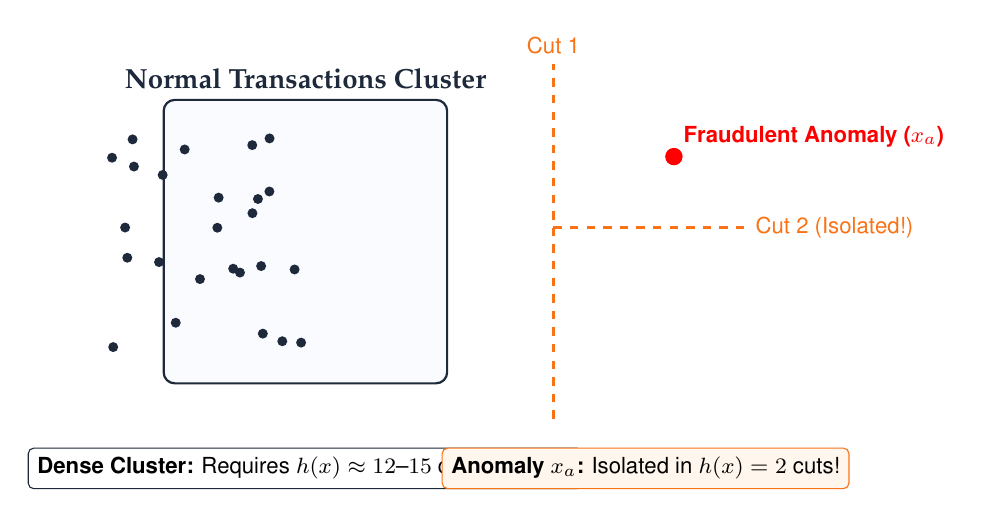
\begin{tikzpicture}[
    scale=0.9,
    font=\sffamily\footnotesize
]

% Normal cluster region
\draw[thick, draw=primarydark, fill=primarylight!40, rounded corners=4pt] (-4, -2) rectangle (0, 2);
\node[color=primarydark, font=\bfseries] at (-2, 2.3) {Normal Transactions Cluster};

% Cluster points
\foreach \i in {1,...,25} {
    \fill[primarydark] (-3.5 + rand*1.5, rand*1.5) circle (2pt);
}

% Anomaly point
\fill[red] (3.2, 1.2) circle (3.5pt) node[above right, color=red] {\textbf{Fraudulent Anomaly ($x_a$)}};

% Partition lines
\draw[dashed, line width=1.2pt, color=coralborder] (1.5, -2.5) -- (1.5, 2.5) node[above] {Cut 1};
\draw[dashed, line width=1.2pt, color=coralborder] (1.5, 0.2) -- (4.2, 0.2) node[right] {Cut 2 (Isolated!)};

% Tree Representation
\node[draw=primarydark, fill=white, rounded corners=2pt] at (-2, -3.2) {\textbf{Dense Cluster:} Requires $h(x) \approx 12$--$15$ cuts to isolate};
\node[draw=coralborder, fill=coralbg, rounded corners=2pt] at (2.8, -3.2) {\textbf{Anomaly $x_a$:} Isolated in $h(x) = 2$ cuts!};

\end{tikzpicture}
\caption{Geometric Partitioning in Isolation Forests: Anomalies Isolate in Few Random Splits.}
\label{fig:isolation_trees}
\end{figure}

% ----------------------------------------------------------------------
% PART 4: DEEP INTUITION & CONCEPTUAL DERIVATIONS
% ----------------------------------------------------------------------
\section{Deep Intuition \& Conceptual Derivations}

\subsection{Why Precision-Recall AUC Dominates ROC-AUC in Fraud Detection}
Under severe class imbalance ($1$ fraud per $1{,}000$ legitimate transactions, $0.1\%$), the standard Receiver Operating Characteristic (ROC) curve presents a deceptively optimistic assessment. 
The ROC curve plots True Positive Rate ($TPR = \frac{TP}{TP+FN}$) against False Positive Rate ($FPR = \frac{FP}{FP+TN}$). 
Because the non-fraud majority class is massive ($TN \approx 999{,}000$):
\begin{equation}
FPR = \frac{FP}{FP + 999{,}000}
\end{equation}
If a model generates $1{,}000$ false positives, the false positive rate remains negligible:
\begin{equation}
FPR = \frac{1000}{1000 + 999000} \approx 0.001 \quad (0.1\%)
\end{equation}
The ROC curve visually hugs the top-left corner, yielding an impressive $\text{ROC-AUC} = 0.98$.
However, evaluate the operational user experience through Precision:
\begin{equation}
\text{Precision} = \frac{TP}{TP + FP} = \frac{100}{100 + 1000} \approx 9.1\%
\end{equation}
Over $90\%$ of alerts investigated by fraud analysts are false alarms! The Precision-Recall curve explicitly exposes this operational breakdown because its denominator ($TP + FP$) directly reflects alert volume.

% ----------------------------------------------------------------------
% PART 5: EXPLICIT GOTCHAS & DIAGNOSTIC MISCONCEPTIONS
% ----------------------------------------------------------------------
\section{Explicit Gotchas \& Diagnostic Misconceptions}

\begin{trapbox}{Gotcha 1: The Accuracy Paradox in Imbalanced Classifiers}
\textbf{The Trap:} Evaluating a fraud machine learning model by celebrating an accuracy score of $99.8\%$.\\
\textbf{Forensic Reality:} In a transaction dataset with $0.1\%$ fraud, a zero-intelligence dummy model that predicts ``Legitimate'' for every single instance achieves $99.9\%$ accuracy while missing $100\%$ of fraudulent transactions. Models must be evaluated strictly using Precision, Recall, $F_2$-score, and PR-AUC.
\end{trapbox}

\begin{trapbox}{Gotcha 2: Applying SMOTE Before Cross-Validation Splitting (Data Leakage)}
\textbf{The Trap:} Applying Synthetic Minority Over-sampling Technique (SMOTE) to the entire dataset before executing $k$-fold cross-validation or train-test splitting.\\
\textbf{Forensic Reality:} Applying SMOTE across the full dataset generates synthetic observations interpolated between training and validation points. Information from the validation set leaks into the training partition, creating artificial test performance that collapses when deployed in production. SMOTE must be fitted exclusively inside each training fold.
\end{trapbox}

\begin{trapbox}{Gotcha 3: Training Unsupervised Anomaly Detectors on Heavily Contaminated Data}
\textbf{The Trap:} Fitting an Isolation Forest on transaction ledgers where organized fraud cartels have operated undetected for months, making up $8\%$ of volume.\\
\textbf{Forensic Reality:} Isolation Forests assume anomalies are few and structurally isolated. When fraudsters execute structured attacks in high volumes, their transactions form dense clusters. The algorithm misinterprets these fraud clusters as normal background activity, masking the scheme completely.
\end{trapbox}

\begin{trapbox}{Gotcha 4: Blindly Retaining Correlated Feature Duplicates}
\textbf{The Trap:} Passing raw transaction attributes (e.g., both total spend and daily spend along with multiple overlapping payment gateway timestamps) into tree boosters without correlation pruning.\\
\textbf{Forensic Reality:} Tree ensembles divide feature importance among collinear covariates, diluting SHAP attributions and creating instability where small data fluctuations alter decision tree splits.
\end{trapbox}

% ----------------------------------------------------------------------
% PART 6: COMPARATIVE SYNTHESIS & SUMMARY TABLE
% ----------------------------------------------------------------------
\section{Comparative Synthesis \& Summary Table}

Table~\ref{tab:comparison_fraud_models} contrasts the core supervised and unsupervised algorithms deployed in production transaction monitoring architectures.

\begin{table}[htbp]
\centering
\small
\begin{tabularx}{\textwidth}{lXXX}
\toprule
\textbf{Model Family} & \textbf{Core Algorithm} & \textbf{Key Advantages} & \textbf{Operational Limitations} \\
\midrule
\textbf{Supervised Boosters} & Gradient Boosted Decision Trees (XGBoost / LightGBM). & Highest tabular discrimination; native handling of missing values; asymmetric loss. & Blind to novel, zero-day fraud attack vectors unrepresented in training labels. \\
\addlinespace
\textbf{Tree Anomaly Detection} & Isolation Forests ($i\text{Forest}$). & Sub-linear $O(n \log n)$ time; zero label requirements; isolates structural outliers. & Vulnerable to dense fraud clusters (masking); sensitive to irrelevant noise features. \\
\addlinespace
\textbf{Density Estimators} & Local Outlier Factor (LOF) / $k$-NN. & Detects local density deviations; identifies isolated transactions in sparse zones. & Computationally prohibitive $O(n^2)$ complexity; unusable for real-time sub-second scoring. \\
\addlinespace
\textbf{Deep Autoencoders} & Deep Reconstruction Neural Networks. & Learns complex non-linear normal manifold; high reconstruction loss flags fraud. & High training compute requirements; requires extensive hyperparameter tuning. \\
\bottomrule
\end{tabularx}
\caption{Systemic Comparison of Machine Learning Paradigms for Financial Fraud Detection.}
\label{tab:comparison_fraud_models}
\end{table}

% ----------------------------------------------------------------------
% PART 7: PYTHON / SCIENTIFIC COMPUTING LAB
% ----------------------------------------------------------------------
\section{Python / Scientific Computing Lab: Supervised vs.~Unsupervised Fraud Pipeline}

Listing~\ref{lst:fraud_ml_engine} implements an end-to-end benchmark comparing a supervised cost-calibrated classifier against an unsupervised Isolation Forest on imbalanced financial transactions.

\begin{lstlisting}[language=Python, caption={Supervised vs.~Unsupervised Transaction Fraud Pipeline in Python}, label={lst:fraud_ml_engine}]
import numpy as np
import pandas as pd
from sklearn.ensemble import IsolationForest
from sklearn.linear_model import LogisticRegression
from sklearn.metrics import classification_report, precision_recall_curve, auc
from sklearn.model_selection import train_test_split

def benchmark_fraud_detectors(X: np.ndarray, y: np.ndarray) -> dict:
    """
    Benchmarks Supervised Logistic Regression against Unsupervised 
    Isolation Forest under extreme class imbalance.
    """
    X_train, X_test, y_train, y_test = train_test_split(
        X, y, test_size=0.3, random_state=42, stratify=y
    )
    
    # 1. Supervised Model with Class Weighting
    supervised_clf = LogisticRegression(class_weight='balanced', max_iter=500)
    supervised_clf.fit(X_train, y_train)
    y_prob_sup = supervised_clf.predict_proba(X_test)[:, 1]
    
    # Precision-Recall AUC for Supervised
    prec_sup, rec_sup, _ = precision_recall_curve(y_test, y_prob_sup)
    pr_auc_sup = auc(rec_sup, prec_sup)
    
    # 2. Unsupervised Model: Isolation Forest (Trained only on unlabeled features)
    # Contamination estimate matching empirical fraud incidence (e.g., 1%)
    iso_forest = IsolationForest(n_estimators=100, contamination=0.01, random_state=42)
    iso_forest.fit(X_train)
    
    # Isolation score: lower values indicate anomalies -> invert for ranking
    anomaly_scores = -iso_forest.score_samples(X_test)
    prec_iso, rec_iso, _ = precision_recall_curve(y_test, anomaly_scores)
    pr_auc_iso = auc(rec_iso, prec_iso)
    
    return {
        'test_frauds': int(y_test.sum()),
        'test_legit': int((1 - y_test).sum()),
        'pr_auc_supervised': round(pr_auc_sup, 4),
        'pr_auc_isolation_forest': round(pr_auc_iso, 4)
    }

# -------------------------------------------------------------
# Test Harness with Synthetic Imbalanced Financial Stream
# -------------------------------------------------------------
if __name__ == '__main__':
    np.random.seed(42)
    n_samples = 10000
    n_fraud = 100  # 1% fraud incidence
    
    # 5 tabular transaction features (Amount, Hour, Distance, Velocity, IP-Risk)
    X_legit = np.random.randn(n_samples - n_fraud, 5)
    # Frauds have shifted means on Amount and Velocity
    X_fraud = np.random.randn(n_fraud, 5) + np.array([3.5, 0.0, 2.0, 4.0, 1.5])
    
    X = np.vstack([X_legit, X_fraud])
    y = np.array([0] * (n_samples - n_fraud) + [1] * n_fraud)
    
    results = benchmark_fraud_detectors(X, y)
    print(f"Test Class Balance: {results['test_frauds']} Frauds / {results['test_legit']} Legit")
    print(f"Supervised PR-AUC: {results['pr_auc_supervised']}")
    print(f"Isolation Forest PR-AUC: {results['pr_auc_isolation_forest']}")
\end{lstlisting}

% ----------------------------------------------------------------------
% PART 8: COMPREHENSIVE PRACTICE PROBLEMS
% ----------------------------------------------------------------------
\section{Comprehensive Practice Problems}
\textit{Complete mathematical derivations and diagnostic MCQ distractor rationales are located in the Appendix.}

\subsection*{Part A: Analytical \& Computational Problems}

\begin{enumerate}[label=\textbf{P9.\arabic*}]
    \item \textbf{The Accuracy Paradox \& Cost-Sensitive Matrix Analysis:}\\
    A fraud detection system evaluates $N = 1{,}000{,}000$ online card transactions. Historical statistics establish that exactly $1{,}000$ transactions ($0.1\%$) are fraudulent. Model $Alpha$ predicts every single transaction is legitimate. Model $Beta$ correctly identifies $800$ frauds, flags $4{,}200$ legitimate transactions as fraud, and misses $200$ frauds.
    \begin{enumerate}[label=(\alph*)]
        \item Compute the Accuracy, Precision, Recall, and $F_1$-score for Model $Alpha$ and Model $Beta$.
        \item Assume the monetary loss of an uncaught fraud is $C_{FN} = \text{Rs.~} 25{,}000$, and the customer friction cost of a false alarm is $C_{FP} = \text{Rs.~} 50$. Compute the total misclassification cost for both models.
        \item Explain why Model $Beta$ is vastly superior despite having a lower raw accuracy score.
    \end{enumerate}

    \item \textbf{Isolation Forest Path Length \& Anomaly Scoring:}\\
    An Isolation Forest algorithm with trees constructed from subsamples of size $n = 256$ evaluates a corporate expense claim.
    \begin{enumerate}[label=(\alph*)]
        \item Compute the average path length normalization factor $c(256)$ using Euler's constant $\gamma \approx 0.5772$.
        \item If a suspicious procurement voucher records an average path length $E[h(x)] = 3.8$ across all trees, calculate its anomaly score $s(x, n)$.
        \item State whether this transaction should be flagged for urgent human audit based on the $s > 0.6$ threshold.
    \end{enumerate}

    \item \textbf{SMOTE Algorithmic Execution \& Geometric Interpolation:}\\
    Consider two minority fraud points in a 2-dimensional feature space: $\mathbf{x}_1 = [2.0, 6.0]^T$ and its nearest minority neighbor $\mathbf{x}_2 = [4.0, 10.0]^T$.
    \begin{enumerate}[label=(\alph*)]
        \item Formulate the SMOTE mathematical generation formula for synthetic instances.
        \item If the random interpolation factor is drawn as $\lambda = 0.35$, compute the exact coordinates of the generated synthetic fraud point $\mathbf{x}_{\text{syn}}$.
        \item Explain why applying SMOTE before train-test partitioning constitutes fatal data leakage.
    \end{enumerate}

    \item \textbf{Precision-Recall Trade-Off \& Operating Threshold Selection:}\\
    A fraud operations center employs $10$ full-time investigators, each capable of reviewing $40$ alerts per day ($400$ daily alert capacity). The bank processes $200{,}000$ daily payments containing an estimated $200$ fraudulent attempts.
    Explain how the risk engineering team should calibrate the model's classification probability cutoff threshold to maximize fraud recovery without overwhelming investigative capacity.

    \item \textbf{Synthetic Identity vs.~Account Takeover Forensics:}\\
    Contrast Synthetic Identity Theft with Account Takeover (ATO) across origin, gestation period, behavioral indicators, and machine learning detection features.
\end{enumerate}

\subsection*{Part B: Diagnostic Multiple-Choice Questions}

\begin{enumerate}[label=\textbf{MCQ 9.\arabic*}]
    \item When training machine learning models on extreme class-imbalanced financial transaction datasets ($0.05\%$ fraud), why is the Precision-Recall Area Under the Curve (PR-AUC) widely preferred over the standard Receiver Operating Characteristic Area Under the Curve (ROC-AUC)?
    \begin{enumerate}[label=(\alph*)]
        \item ROC-AUC is mathematically undefined when classes are imbalanced.
        \item ROC-AUC includes the massive True Negative class in the False Positive Rate denominator ($FPR = \frac{FP}{FP + TN}$), causing the metric to look deceptively near-perfect even when thousands of false positive alerts overwhelm analysts.
        \item PR-AUC guarantees that the model has zero False Negatives.
        \item Tree-based models like XGBoost can only compute Precision-Recall curves.
    \end{enumerate}

    \item In the mathematical formulation of the Isolation Forest anomaly detector, what does an average path length $E[h(x)] \ll c(n)$ signify for a specific transaction instance $x$?
    \begin{enumerate}[label=(\alph*)]
        \item The transaction is surrounded by a dense cluster of identical normal records.
        \item The transaction is an isolated structural anomaly that required very few random feature splits to be separated from the rest of the dataset.
        \item The transaction contains corrupted null values that broke the binary search tree.
        \item The transaction balance satisfies Benford's Law distribution.
    \end{enumerate}
\end{enumerate}

\chapter{Time Series Analysis \& Temporal Anomaly Detection}

\begin{tcolorbox}[colback=primarylight, colframe=primarydark, title={\textbf{What You Will Learn in this Chapter}}]
\begin{itemize}
    \item Foundations of temporal financial data: High-frequency transaction velocity and settlement flows
    \item Classical decomposition: Trend ($T_t$), Seasonality ($S_t$), and Irregular noise ($\epsilon_t$)
    \item Weak stationarity conditions and unit-root testing via Augmented Dickey-Fuller (ADF)
    \item Mathematical structure of Autoregressive Integrated Moving Average (ARIMA) models
    \item Statistical process control: Dynamic rolling-window confidence bounds and CUSUM change-point detection
    \item Hands-on Python implementation of ARIMA residual forecasting and withdrawal burst detection
\end{itemize}
\end{tcolorbox}

\section{The Temporal Dimension of Financial Forensics}

Financial transactions do not occur as independent, identically distributed (i.i.d.) static observations; they are dynamic \index{time series}\textbf{time series} indexed sequentially in time: $\{y_t\}_{t=1}^T$. Forensic investigators analyze temporal series to detect abrupt structural shifts, unusual volume bursts, and money laundering layering spikes.

\begin{definitionbox}{Classical Time Series Decomposition}
\index{Time Series Decomposition}
A financial time series $y_t$ can be decomposed into additive or multiplicative components:
\begin{align}
\text{Additive:} \quad y_t &= T_t + S_t + C_t + \epsilon_t \\
\text{Multiplicative:} \quad y_t &= T_t \times S_t \times C_t \times \epsilon_t
\end{align}
where $T_t$ represents the long-term secular trend, $S_t$ is deterministic periodic seasonality (e.g., end-of-month payroll spikes), $C_t$ is cyclical macroeconomic variation, and $\epsilon_t$ is stochastic white noise.
\end{definitionbox}

\begin{videocard}{IITM BS Lecture: Introduction to Time Series}{https://www.youtube.com/watch?v=odptnlDEz8U}
Understanding temporal dependencies in finance, timestamp sequencing, and frequency aggregation.
\end{videocard}

\begin{videocard}{IITM BS Lecture: Components of Time Series}{https://www.youtube.com/watch?v=0CIdS0syn34}
Decomposing financial signals into underlying trends, seasonal patterns, and residual error terms.
\end{videocard}

\section{Stationarity and the Augmented Dickey-Fuller Test}

A time series is said to be \index{stationarity}\textbf{weakly (covariance) stationary} if its statistical properties do not change over time:
\begin{enumerate}
    \item Constant expected value: $E[y_t] = \mu$ for all $t$.
    \item Constant finite variance: $\text{Var}(y_t) = \sigma^2 < \infty$ for all $t$.
    \item Autocovariance depends only on lag $k$, not on time $t$: $\text{Cov}(y_t, y_{t-k}) = \gamma_k$.
\end{enumerate}

\begin{videocard}{Masterclass Video: Stationarity in Time Series -- Ritvikmath}{https://www.youtube.com/watch?v=oY-j2Wof51c}
Ritvikmath's visual explanation of why non-stationary time series generate spurious correlations and how differencing achieves stationarity.
\end{videocard}

\begin{theorembox}{The Augmented Dickey-Fuller (ADF) Test}
\index{Augmented Dickey-Fuller Test}
To test for the presence of a unit root (non-stationarity), estimate the regression:
\begin{equation}
\Delta y_t = \alpha + \beta t + \gamma y_{t-1} + \sum_{i=1}^p \delta_i \Delta y_{t-i} + \epsilon_t
\end{equation}
The hypothesis test is formulated as:
\begin{itemize}
    \item $H_0: \gamma = 0$ (The series possesses a unit root and is non-stationary).
    \item $H_1: \gamma < 0$ (The series is stationary).
\end{itemize}
If the ADF test-statistic is more negative than the critical value (or $p < 0.05$), we reject $H_0$ and conclude the series is stationary.
\end{theorembox}

\section{ARIMA Modeling for Baseline Forecasting}

To detect temporal anomalies, forensic engines fit an \index{ARIMA}\textbf{Autoregressive Integrated Moving Average (ARIMA$(p, d, q)$)} model on historical baseline behavior.

\begin{formulabox}{ARIMA$(p, d, q)$ Formulation}
For a $d$-times differenced series $y_t' = \nabla^d y_t$:
\begin{equation}
y_t' = c + \sum_{i=1}^p \phi_i y_{t-i}' + \sum_{j=1}^q \theta_j \epsilon_{t-j} + \epsilon_t
\end{equation}
where $\phi_1, \dots, \phi_p$ are autoregressive coefficients, $\theta_1, \dots, \theta_q$ are moving average coefficients, and $\epsilon_t \sim \mathcal{N}(0, \sigma^2)$ is Gaussian white noise.
\end{formulabox}

\begin{videocard}{IITM BS Lecture: Time Series Models}{https://www.youtube.com/watch?v=rHDKwLcsM2o}
Mathematical specification of AR, MA, ARMA, and seasonal ARIMA models for financial forecasting.
\end{videocard}

\begin{videocard}{IITM BS Lecture: Time Series Models -- Hands-On}{https://www.youtube.com/watch?v=3LI8ziBMVJ0}
Practical tutorial using Python statsmodels to fit ARIMA models, analyze ACF/PACF plots, and inspect residuals.
\end{videocard}

\section{Temporal Anomaly Detection: Dynamic Confidence Intervals and CUSUM}

Once an ARIMA model is trained on legitimate baseline history, it generates one-step-ahead forecasts $\hat{y}_t$ with conditional variance $\sigma_t^2$.

\begin{intuitionbox}{The Dynamic Forensic Envelope}
Static thresholds (e.g., ``flag any withdrawal $> \text{Rs.~5,00,000}$'') fail because normal business payroll spikes on the 1st of every month get flagged, while an illicit Rs.~3,00,000 extraction on a quiet Sunday afternoon passes undetected. An ARIMA confidence envelope expands during expected high-volatility hours and contracts during quiet periods, exposing stealthy off-hour transactions.
\end{intuitionbox}

\begin{definitionbox}{CUSUM (Cumulative Sum Control Chart)}
\index{CUSUM}
CUSUM monitors cumulative positive and negative deviations from the baseline mean $\mu_0$:
\begin{align}
S_t^+ &= \max\left(0, S_{t-1}^+ + (y_t - \mu_0) - K\right) \\
S_t^- &= \max\left(0, S_{t-1}^- - (y_t - \mu_0) - K\right)
\end{align}
where $K$ is the allowable tolerance parameter. An anomaly alarm fires if $S_t^+ > H$ or $S_t^- > H$, detecting persistent micro-leakage (such as salami slicing fraud).
\end{definitionbox}

\begin{figure}[htbp]
\centering
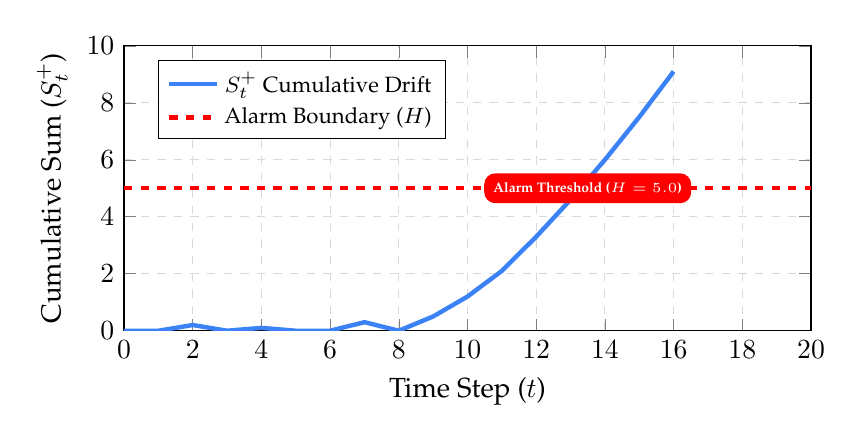
\begin{tikzpicture}
\begin{axis}[
    width=0.85\textwidth,
    height=5.2cm,
    xmin=0, xmax=20,
    ymin=0, ymax=10,
    xlabel={Time Step ($t$)},
    ylabel={Cumulative Sum ($S_t^+$)},
    grid=major,
    grid style={dashed, gray!30},
    legend style={at={(0.05,0.95)}, anchor=north west, font=\footnotesize}
]
\addplot[ultra thick, primaryborder] coordinates {
    (0,0) (1,0) (2,0.2) (3,0) (4,0.1) (5,0) (6,0) (7,0.3) 
    (8,0) (9,0.5) (10,1.2) (11,2.1) (12,3.3) (13,4.6) (14,6.0) (15,7.5) (16,9.1)
};
\addplot[dashed, ultra thick, red] coordinates {(0,5.0) (20,5.0)};
\node[fill=red, text=white, rounded corners, font=\tiny\bfseries] at (axis cs:13.5,5.0) {Alarm Threshold ($H=5.0$)};
\legend{$S_t^+$ Cumulative Drift, Alarm Boundary ($H$)}
\end{axis}
\end{tikzpicture}
\caption{CUSUM Control Chart: Detecting Persistent Low-Magnitude Siphoning (Salami Slicing) Crossing the Alarm Limit $H$.}
\end{figure}

\section{Data Science Relevance: Temporal Residual Anomaly Detection}

\begin{lstlisting}[caption={Time Series Residual Anomaly Detection in Python}]
import numpy as np
import pandas as pd
from statsmodels.tsa.arima.model import ARIMA
from statsmodels.tsa.stattools import adfuller

# Simulate 120 days of daily withdrawal volumes (in Rs. Thousands)
np.random.seed(42)
days = pd.date_range(start='2026-01-01', periods=120, freq='D')
base_signal = 100.0 + np.sin(np.arange(120) * (2 * np.pi / 7)) * 15.0 # Weekly cycle
noise = np.random.normal(0, 5, 120)
withdrawals = base_signal + noise

# Inject sudden fraudulent cash drain anomalies on Day 85 and Day 86
withdrawals[85] += 65.0  # Massive spike
withdrawals[86] += 70.0

ts_df = pd.DataFrame({'date': days, 'amount': withdrawals}).set_index('date')

# 1. ADF Test for Stationarity
adf_res = adfuller(ts_df['amount'])
print(f"ADF Statistic: {adf_res[0]:.3f}, p-value: {adf_res[1]:.4e}")

# 2. Fit ARIMA(1, 0, 1) model on baseline (first 75 days)
train_series = ts_df['amount'].iloc[:75]
model = ARIMA(train_series, order=(1, 0, 1))
fitted_model = model.fit()

# 3. Dynamic Residual Forecasting on full series
preds = fitted_model.predict(start=0, end=len(ts_df)-1)
residuals = ts_df['amount'] - preds
residual_std = residuals.iloc[:75].std()

# 4. Flag residuals exceeding 3 standard deviations
ts_df['forecast'] = preds
ts_df['residual'] = residuals
ts_df['anomaly_flag'] = np.abs(residuals) > (3.0 * residual_std)

anomalies = ts_df[ts_df['anomaly_flag']]
print(f"\nDetected {len(anomalies)} Temporal Anomalies:")
print(anomalies[['amount', 'forecast', 'residual']])
\end{lstlisting}

\section*{Supplementary Lecture Videos}
\begin{itemize}
    \item \href{https://www.youtube.com/watch?v=odptnlDEz8U}{W10\_L1: Introduction to Time Series in Financial Forensics}
    \item \href{https://www.youtube.com/watch?v=0CIdS0syn34}{W10\_L2: Components of Time Series (Trend, Seasonality, Noise)}
    \item \href{https://www.youtube.com/watch?v=rHDKwLcsM2o}{W10\_L3: Time Series Models (AR, MA, ARMA, ARIMA)}
    \item \href{https://www.youtube.com/watch?v=3LI8ziBMVJ0}{W10\_L4: Time Series Models -- Hands-On Python Tutorial}
    \item \href{https://www.youtube.com/watch?v=oY-j2Wof51c}{External Masterclass: Stationarity in Time Series (Ritvikmath)}
\end{itemize}

\newpage
\section{Practice Exercises}
\textit{Detailed step-by-step solutions are available in the Appendix.}

\begin{enumerate}
    \item Define covariance stationarity. Given the first-order autoregressive process:
    \begin{equation*}
    y_t = \delta + \phi_1 y_{t-1} + \epsilon_t, \quad \epsilon_t \sim \mathcal{WN}(0, \sigma^2)
    \end{equation*}
    derive the unconditional mean $E[y_t]$ and the unconditional variance $\text{Var}(y_t)$ under the stability condition $|\phi_1| < 1$. What happens if $\phi_1 = 1$?
    
    \item An Augmented Dickey-Fuller test conducted on daily transaction count data yields a test statistic of $-1.82$. If the critical value at the $5\%$ significance level is $-2.89$, state the statistical conclusion. What data transformation is required before fitting an ARMA model?
    
    \item Explain how an adversary executes a ``salami slicing'' fraud scheme (repeatedly siphoning fractions of a cent or a few rupees from millions of customer accounts). Why does standard outlier detection fail to catch this, and how does the CUSUM algorithm detect it?
    
    \item Given an ARIMA$(0, 1, 1)$ model formulated as:
    \begin{equation*}
    y_t - y_{t-1} = \epsilon_t - \theta_1 \epsilon_{t-1}
    \end{equation*}
    show that the one-step-ahead point forecast $\hat{y}_{t+1|t}$ can be expressed as an exponentially weighted moving average (EWMA) of past historical observations.
    
    \item Describe the difference between additive and multiplicative seasonal decomposition in time series. Under what operational conditions in corporate cash flows is multiplicative decomposition required?
\end{enumerate}

\chapter{Forensic Text Mining, NLP \& Entity Resolution}

% ----------------------------------------------------------------------
% PART 1: EXECUTIVE ROADMAP & LEARNING OBJECTIVES
% ----------------------------------------------------------------------
\section{Executive Roadmap \& Learning Objectives}

While quantitative transaction databases record numerical accounting values, over $80\%$ of actionable enterprise intelligence resides within unstructured text: regulatory disclosures (e.g., SEC Form 10-K or SEBI annual reports), internal audit memorandums, executive email archives, and wire transfer payment narrations. In forensic accounting and Anti-Money Laundering (AML) investigations, unstructured text reveals critical deception markers, undisclosed related-party dealings, and adversarial name obfuscation used to circumvent international sanctions.

\begin{tcolorbox}[colback=primarylight, colframe=primarydark, title={\textbf{Core Learning Competencies}}]
Upon mastering this chapter, students will be equipped to:
\begin{itemize}
    \item \textbf{Mine Deceptive Linguistic Signatures:} Extract psycholinguistic indicators of executive deception within Management Discussion \& Analysis (MD\&A) disclosures using specialized financial dictionaries.
    \item \textbf{Engineer Text Representation Pipelines:} Apply tokenization, lemmatization, and Term Frequency-Inverse Document Frequency (TF-IDF) transformations to unstructured corporate text.
    \item \textbf{Execute Named Entity Recognition (NER):} Isolate company entities, offshore jurisdictions, and Politically Exposed Persons (PEPs) from dense narrative filings.
    \item \textbf{Resolve Entity Disambiguation Challenges:} Formulate string distance metrics (Levenshtein, Jaro-Winkler) and phonetic hashing algorithms to link obscured shell company names.
    \item \textbf{Deploy Scalable Record Linkage Pipelines:} Implement blocking and indexing architectures in Python to execute entity resolution across large vendor ledgers.
\end{itemize}
\end{tcolorbox}

\begin{table}[htbp]
\centering
\small
\begin{tabularx}{\textwidth}{llX}
\toprule
\textbf{Construct / Metric} & \textbf{Symbol} & \textbf{Mathematical Definition / Structural Formula} \\
\midrule
Term Frequency & $\text{TF}(t, d)$ & $\frac{f_{t,d}}{\sum_{t' \in d} f_{t',d}} \quad \text{or raw count } f_{t,d}$ \\
Inverse Document Freq & $\text{IDF}(t, D)$ & $\ln\left(\frac{1 + |D|}{1 + |\{d \in D : t \in d\}|}\right) + 1$ \\
TF-IDF Weight & $w_{t,d}$ & $\text{TF}(t, d) \times \text{IDF}(t, D)$ \\
Cosine Text Similarity & $\text{Sim}_{\cos}(\mathbf{u}, \mathbf{v})$ & $\frac{\mathbf{u} \cdot \mathbf{v}}{\|\mathbf{u}\|_2 \|\mathbf{v}\|_2} = \frac{\sum u_i v_i}{\sqrt{\sum u_i^2} \sqrt{\sum v_i^2}}$ \\
Levenshtein Distance & $\text{Lev}(s_1, s_2)$ & Minimum insertions, deletions, substitutions to transform $s_1 \to s_2$ \\
Jaro Distance & $Sim_J(s_1, s_2)$ & $\frac{1}{3} \left(\frac{m}{|s_1|} + \frac{m}{|s_2|} + \frac{m - t}{m}\right)$ \\
Jaro-Winkler & $Sim_{JW}(s_1, s_2)$ & $Sim_J + \ell p (1 - Sim_J) \quad (\ell \le 4, p = 0.1)$ \\
\bottomrule
\end{tabularx}
\caption{Mathematical Notation Guide for Forensic NLP and Entity Resolution.}
\label{tab:w11_notation}
\end{table}

% ----------------------------------------------------------------------
% PART 2: MATHEMATICAL & COMPUTATIONAL FOUNDATIONS
% ----------------------------------------------------------------------
\section{Mathematical \& Computational Foundations}

\subsection{The TF-IDF Vector Space Model}
To analyze unstructured financial disclosures, text corpora are converted into numerical feature vectors. The weight of term $t$ in document $d$ within corpus $D$ is:
\begin{equation}
w_{t,d} = \text{TF}(t, d) \times \text{IDF}(t, D)
\label{eq:tfidf_formula}
\end{equation}
In forensic linguistics, specialized dictionaries (e.g., the Loughran-McDonald Financial Sentiment Dictionary) supersede generic sentiment lexicons, classifying corporate text across six forensic dimensions: Negative, Positive, Uncertainty, Litigious, Constraining, and Superfluous.

\subsection{String Distance Metrics for Entity Disambiguation}
Adversaries intentionally introduce typographical alterations to disguise shell companies (e.g., ``Satyam Infoway Ltd'' vs.~``Satyam Info-Way Limited'').

\subsubsection{1. Levenshtein Edit Distance}
For strings $s_1$ and $s_2$ of lengths $|s_1|$ and $|s_2|$, the edit distance $D(i, j)$ satisfies the dynamic programming recurrence:
\begin{equation}
D(i, j) = \begin{cases}
\max(i, j) & \text{if } \min(i, j) = 0, \\
\min \begin{cases}
D(i - 1, j) + 1 \\
D(i, j - 1) + 1 \\
D(i - 1, j - 1) + \mathbb{I}(s_1[i] \ne s_2[j])
\end{cases} & \text{otherwise.}
\end{cases}
\label{eq:levenshtein}
\end{equation}
The normalized similarity score is:
\begin{equation}
\text{Sim}_{\text{Lev}}(s_1, s_2) = 1 - \frac{\text{Lev}(s_1, s_2)}{\max(|s_1|, |s_2|)} \in [0, 1]
\end{equation}

\subsubsection{2. Jaro-Winkler Metric for Enterprise Names}
For strings $s_1$ and $s_2$, let $m$ be the number of matching characters within distance $\lfloor \frac{\max(|s_1|, |s_2|)}{2} \rfloor - 1$, and let $t$ be the number of transpositions. The Jaro metric is:
\begin{equation}
Sim_J = \begin{cases}
0 & \text{if } m = 0, \\
\frac{1}{3}\left(\frac{m}{|s_1|} + \frac{m}{|s_2|} + \frac{m - t}{m}\right) & \text{otherwise.}
\end{cases}
\label{eq:jaro}
\end{equation}
The Jaro-Winkler extension rewards matching common initial prefixes:
\begin{equation}
Sim_{JW} = Sim_J + \ell \cdot p \cdot (1 - Sim_J)
\label{eq:jaro_winkler}
\end{equation}
where $\ell \le 4$ is the length of the common prefix and $p = 0.1$ is the constant scaling factor.

% ----------------------------------------------------------------------
% PART 3: VISUAL & GEOMETRIC INTUITION
% ----------------------------------------------------------------------
\section{Visual \& Geometric Intuition: The Entity Resolution Architecture}

Figure~\ref{fig:entity_resolution} diagrams the end-to-end entity resolution pipeline, illustrating how raw, noisy vendor records are normalized, blocked, and scored to unmask hidden shell company networks.

\begin{figure}[htbp]
\centering
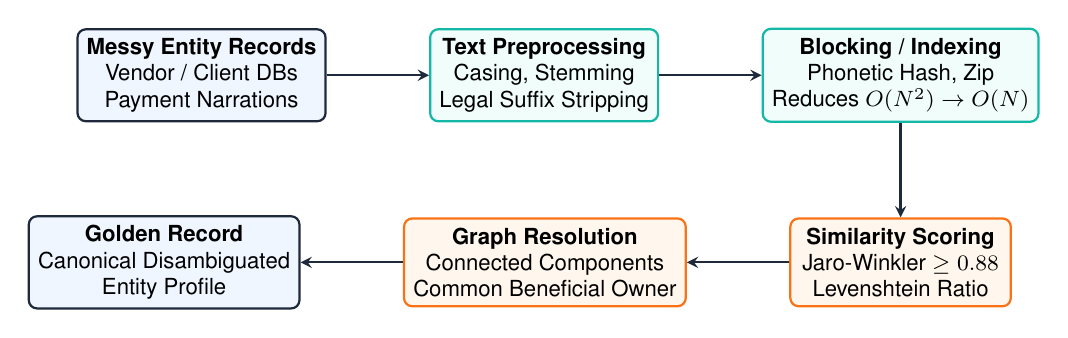
\begin{tikzpicture}[
    font=\sffamily\footnotesize,
    node distance=1.1cm and 1.3cm,
    block/.style={rectangle, draw=primarydark, fill=primarylight, thick, rounded corners=3pt, minimum width=2.8cm, minimum height=1.1cm, align=center},
    action/.style={rectangle, draw=tealborder, fill=tealbg, thick, rounded corners=3pt, minimum width=2.8cm, minimum height=1.1cm, align=center},
    alert/.style={rectangle, draw=coralborder, fill=coralbg, thick, rounded corners=3pt, minimum width=2.8cm, minimum height=1.1cm, align=center},
    arr/.style={->, >=stealth, thick, color=primarydark}
]

% Nodes
\node[block] (raw) {\textbf{Messy Entity Records}\\Vendor / Client DBs\\Payment Narrations};
\node[action, right=of raw] (prep) {\textbf{Text Preprocessing}\\Casing, Stemming\\Legal Suffix Stripping};
\node[action, right=of prep] (block) {\textbf{Blocking / Indexing}\\Phonetic Hash, Zip\\Reduces $O(N^2) \to O(N)$};
\node[alert, below=1.2cm of block] (score) {\textbf{Similarity Scoring}\\Jaro-Winkler $\ge 0.88$\\Levenshtein Ratio};
\node[alert, left=of score] (graph) {\textbf{Graph Resolution}\\Connected Components\\Common Beneficial Owner};
\node[block, left=of graph] (out) {\textbf{Golden Record}\\Canonical Disambiguated\\Entity Profile};

% Connectors
\draw[arr] (raw) -- (prep);
\draw[arr] (prep) -- (block);
\draw[arr] (block) -- (score);
\draw[arr] (score) -- (graph);
\draw[arr] (graph) -- (out);

\end{tikzpicture}
\caption{The Automated Forensic Entity Resolution and Record Linkage Pipeline.}
\label{fig:entity_resolution}
\end{figure}

% ----------------------------------------------------------------------
% PART 4: DEEP INTUITION & CONCEPTUAL DERIVATIONS
% ----------------------------------------------------------------------
\section{Deep Intuition \& Conceptual Derivations}

\subsection{Linguistic Deception in Corporate Annual Filings}
In empirical forensic accounting literature (e.g., Larcker and Zakolyukina, 2012), deceptive corporate disclosures exhibit three statistically significant psycholinguistic traits:
\begin{enumerate}
    \item \textbf{First-Person Pronoun Displacement:} Executives intentionally suppress self-referential pronouns (``I'', ``we'', ``my'') and substitute third-person institutional terminology (``the company'', ``management'', ``the board''). This reflects psychological distancing from statements the executive knows to be false.
    \item \textbf{Cognitive Complexity and Gunning Fog Inflation:} When performance deteriorates, deceptive disclosures feature complex sentence structures, Latinate legalisms, and passive voice phrasing to increase cognitive reading latency.
    \item \textbf{Extreme Positive Sentiment Asymmetry:} Deceptive annual reports feature an unnatural frequency of extreme positive superlatives (``unparalleled'', ``unprecedented'') designed to rhetorically counter deteriorating financial ratios.
\end{enumerate}

% ----------------------------------------------------------------------
% PART 5: EXPLICIT GOTCHAS & DIAGNOSTIC MISCONCEPTIONS
% ----------------------------------------------------------------------
\section{Explicit Gotchas \& Diagnostic Misconceptions}

\begin{trapbox}{Gotcha 1: Neglecting Domain-Specific Financial Sentiment Dictionaries}
\textbf{The Trap:} Applying generic natural language sentiment packages (e.g., VADER or TextBlob) directly to corporate financial filings.\\
\textbf{Forensic Reality:} In general English, words like ``liability'', ``depreciation'', ``tax'', ``board'', and ``share'' carry negative or neutral connotations. Standard lexicons misclassify normal corporate accounting passages as overwhelmingly negative. Forensic NLP must utilize the Loughran-McDonald dictionary, which properly calibrates financial semantics.
\end{trapbox}

\begin{trapbox}{Gotcha 2: The Exact-Match Blindspot in Sanctions Screening}
\textbf{The Trap:} Screening international wire transfer payees against global AML sanctions lists using exact SQL \texttt{WHERE} string matching.\\
\textbf{Forensic Reality:} Illicit actors deliberately insert subtle typographical variations (e.g., swapping Cyrillic lookalike letters or changing ``Mohammad'' to ``Muhamed''). Exact-match queries produce a $100\%$ evasion rate. Automated fuzzy string matching and phonetic algorithms are legally mandated under FATF recommendations.
\end{trapbox}

\begin{trapbox}{Gotcha 3: The Quadratic Complexity Explosion in Record Linkage}
\textbf{The Trap:} Executing pairwise Levenshtein or Jaro-Winkler distance computations across all record pairs in an enterprise ledger of $N = 500{,}000$ transactions.\\
\textbf{Forensic Reality:} The total number of pairwise comparisons scales as $\binom{N}{2} = \frac{N(N-1)}{2} \approx 1.25 \times 10^{11}$ operations, overwhelming server clusters. Scalable entity resolution requires **blocking** (e.g., partitioning records by soundex code, state, or initial characters) to restrict pairwise comparison to plausible candidates ($O(N)$).
\end{trapbox}

\begin{trapbox}{Gotcha 4: Relying Solely on Soundex Phonetic Hashing for Transliterated Names}
\textbf{The Trap:} Utilizing the classic Soundex phonetic algorithm to match international corporate entities and foreign beneficial owners.\\
\textbf{Forensic Reality:} Soundex was engineered in the early 20th century specifically for American Census English surnames. It handles Asian, Arabic, Slavic, and African name transliterations exceptionally poorly. Modern systems require Double Metaphone or deep embedding neural string encodings.
\end{trapbox}

% ----------------------------------------------------------------------
% PART 6: COMPARATIVE SYNTHESIS & SUMMARY TABLE
% ----------------------------------------------------------------------
\section{Comparative Synthesis \& Summary Table}

Table~\ref{tab:comparison_string_metrics} compares the computational performance, typo resilience, and forensic suitability of core entity resolution algorithms.

\begin{table}[htbp]
\centering
\small
\begin{tabularx}{\textwidth}{lXXX}
\toprule
\textbf{String Metric} & \textbf{Algorithm Logic} & \textbf{Prefix / Transposition Sensitivity} & \textbf{Primary Forensic Application} \\
\midrule
\textbf{Levenshtein Ratio} & Dynamic programming edit matrix counting insertions, deletions, edits. & Uniform across the entire string length; sensitive to character order. & Document tampering; contract clause alterations; invoice number typos. \\
\addlinespace
\textbf{Jaro-Winkler} & Matches characters within sliding window with weighted bonus for prefix. & High bonus for matching initial 4 characters; penalizes suffix differences. & Person and business entity matching; AML sanctions list screening. \\
\addlinespace
\textbf{Double Metaphone} & Phonetic encoding mapping words to approximate pronunciation codes. & Invariant to spelling variations that produce identical acoustic sound. & Cross-lingual customer deduplication; informal payment narrations. \\
\addlinespace
\textbf{TF-IDF Cosine} & Bag-of-words vector angle normalized by global corpus frequency. & Completely order-invariant; sensitive to distinctive, rare vocabulary. & Matching multi-word corporate names; unstructured regulatory filings. \\
\bottomrule
\end{tabularx}
\caption{Systemic Comparison of String Similarity Metrics in Forensic Entity Resolution.}
\label{tab:comparison_string_metrics}
\end{table}

% ----------------------------------------------------------------------
% PART 7: PYTHON / SCIENTIFIC COMPUTING LAB
% ----------------------------------------------------------------------
\section{Python / Scientific Computing Lab: Automated Entity Resolution Engine}

Listing~\ref{lst:nlp_entity_engine} provides an automated Python program that performs text normalization, phonetic blocking, Jaro-Winkler similarity scoring, and resolves messy procurement vendor identities.

\begin{lstlisting}[language=Python, caption={Automated Vendor Entity Resolution Engine in Python}, label={lst:nlp_entity_engine}]
import re
from typing import List, Tuple

def clean_entity_name(name: str) -> str:
    """
    Standardizes commercial entity names by stripping legal suffixes,
    punctuation, and excess whitespace.
    """
    name = name.lower()
    # Remove common legal business entities
    legal_suffixes = r'\b(ltd|limited|inc|incorporated|corp|corporation|pvt|private|llc|co)\b'
    name = re.sub(legal_suffixes, '', name)
    # Remove special punctuation
    name = re.sub(r'[^a-z0-9\s]', '', name)
    return ' '.join(name.split())

def jaro_distance(s1: str, s2: str) -> float:
    """Computes standard Jaro distance between two strings."""
    if s1 == s2:
        return 1.0
    len1, len2 = len(s1), len(s2)
    if len1 == 0 or len2 == 0:
        return 0.0
        
    match_distance = max(len1, len2) // 2 - 1
    s1_matches = [False] * len1
    s2_matches = [False] * len2
    matches = 0
    
    for i in range(len1):
        start = max(0, i - match_distance)
        end = min(i + match_distance + 1, len2)
        for j in range(start, end):
            if not s2_matches[j] and s1[i] == s2[j]:
                s1_matches[i] = True
                s2_matches[j] = True
                matches += 1
                break
                
    if matches == 0:
        return 0.0
        
    transpositions = 0
    k = 0
    for i in range(len1):
        if s1_matches[i]:
            while not s2_matches[k]:
                k += 1
            if s1[i] != s2[k]:
                transpositions += 1
            k += 1
            
    t = transpositions / 2.0
    return (matches / len1 + matches / len2 + (matches - t) / matches) / 3.0

def jaro_winkler(s1: str, s2: str, p: float = 0.1) -> float:
    """Computes Jaro-Winkler similarity with prefix bonus."""
    j = jaro_distance(s1, s2)
    # Common prefix up to 4 characters
    prefix = 0
    for c1, c2 in zip(s1[:4], s2[:4]):
        if c1 == c2:
            prefix += 1
        else:
            break
    return j + prefix * p * (1.0 - j)

def resolve_vendor_records(query_name: str, candidate_catalog: List[str], threshold: float = 0.85) -> List[Tuple[str, float]]:
    """Matches a messy vendor query against a clean master vendor catalog."""
    clean_query = clean_entity_name(query_name)
    matches = []
    
    for candidate in candidate_catalog:
        clean_cand = clean_entity_name(candidate)
        sim = jaro_winkler(clean_query, clean_cand)
        if sim >= threshold:
            matches.append((candidate, round(sim, 4)))
            
    matches.sort(key=lambda x: x[1], reverse=True)
    return matches

# -------------------------------------------------------------
# Test Harness with Real-World Shell Entity Variations
# -------------------------------------------------------------
if __name__ == '__main__':
    master_catalog = [
        "Hindustan Logistics Private Limited",
        "Satyam Infoway Corporation",
        "Tata Consultancy Services Ltd",
        "Bharat Heavy Electricals Limited"
    ]
    
    suspicious_queries = [
        "Hindostan Logistics Pvt Ltd",
        "Satyam Info-Way Corp",
        "TCS Ltd.",
        "Random Ghost Shell Co"
    ]
    
    print("Forensic Entity Resolution Matching Results:")
    for query in suspicious_queries:
        matched = resolve_vendor_records(query, master_catalog, threshold=0.82)
        if matched:
            best_match, score = matched[0]
            print(f"Query: '{query}' -> Match: '{best_match}' (Similarity: {score})")
        else:
            print(f"Query: '{query}' -> NO MATCH (Unregistered / Novel Entity)")
\end{lstlisting}

% ----------------------------------------------------------------------
% PART 8: COMPREHENSIVE PRACTICE PROBLEMS
% ----------------------------------------------------------------------
\section{Comprehensive Practice Problems}
\textit{Complete mathematical derivations and diagnostic MCQ distractor rationales are located in the Appendix.}

\subsection*{Part A: Analytical \& Computational Problems}

\begin{enumerate}[label=\textbf{P11.\arabic*}]
    \item \textbf{TF-IDF Weighting \& Deceptive Corpus Scoring:}\\
    An internal audit investigation reviews a corpus of $N = 1{,}000$ executive emails. The term \texttt{unprecedented} appears $6$ times in a suspect CFO email of $200$ total words. Across the entire corpus, \texttt{unprecedented} appears in only $10$ emails.
    \begin{enumerate}[label=(\alph*)]
        \item Compute the Term Frequency ($\text{TF}$) of the term in the suspect email.
        \item Compute the natural Inverse Document Frequency ($\text{IDF}$) using the smoothed formulation $\ln\left(\frac{1 + N}{1 + \text{DF}}\right) + 1$.
        \item Compute the final TF-IDF score.
        \item Explain why rare, emotionally hyperbolic words achieve high TF-IDF scores in forensic text mining.
    \end{enumerate}

    \item \textbf{Step-by-Step Levenshtein Edit Distance Matrix:}\\
    A fraudulent wire transfer specifies the beneficiary bank account holder as \texttt{SATYAM}. The legitimate authorized master vendor name on record is \texttt{SATNAM}.
    \begin{enumerate}[label=(\alph*)]
        \item Construct the complete dynamic programming $(7 \times 7)$ Levenshtein distance matrix.
        \item State the final minimum edit distance $\text{Lev}(\texttt{SATYAM}, \texttt{SATNAM})$.
        \item Calculate the normalized Levenshtein similarity percentage.
    \end{enumerate}

    \item \textbf{Jaro-Winkler Calculation for Shell Entity Matching:}\\
    An AML screening engine compares two vendor names: $s_1 = \texttt{BHARAT}$ and $s_2 = \texttt{BHARTY}$.
    \begin{enumerate}[label=(\alph*)]
        \item Determine the maximum allowable match distance.
        \item Identify the matching characters and count the number of transpositions.
        \item Compute the base Jaro distance $Sim_J$.
        \item Determine the common prefix length $\ell$ and compute the final Jaro-Winkler similarity $Sim_{JW}$ using $p = 0.1$.
    \end{enumerate}

    \item \textbf{Linguistic Deception \& MD\&A Risk Profiling:}\\
    Two pharmaceutical firms publish their annual MD\&A disclosures. Firm $A$ reports a first-person pronoun frequency of $0.2\%$, an average sentence length of $38$ words, and a Loughran-McDonald uncertainty word density of $4.8\%$. Firm $B$ reports $1.8\%$ first-person pronouns, $18$ words per sentence, and $1.1\%$ uncertainty terms. Formulate an investigative assessment regarding which firm presents elevated financial reporting deception risk.

    \item \textbf{Scalable Blocking Strategy in Corporate Registry Linkage:}\\
    A national financial intelligence unit must match $2{,}000{,}000$ offshore corporate registry records against $500{,}000$ domestic bank accounts. Detail a multi-pass blocking architecture utilizing phonetic hashing and geographic indexing to ensure computational feasibility.
\end{enumerate}

\subsection*{Part B: Diagnostic Multiple-Choice Questions}

\begin{enumerate}[label=\textbf{MCQ 11.\arabic*}]
    \item In forensic text mining of corporate annual reports, why do domain-specific dictionaries like the Loughran-McDonald financial lexicon dramatically outperform generic sentiment tools such as VADER or TextBlob?
    \begin{enumerate}[label=(\alph*)]
        \item Generic lexicons misclassify standard recurring corporate financial terminology (e.g., ``depreciation'', ``tax'', ``liability'') as negative sentiment, generating massive false-positive deception signals.
        \item Generic lexicons cannot process English words with more than six letters.
        \item The Loughran-McDonald dictionary converts text into double-entry journal vouchers.
        \item The Securities and Exchange Commission mandates that all models achieve $100\%$ accuracy.
    \end{enumerate}

    \item In string similarity calculations for entity resolution, how does the Jaro-Winkler metric modify the standard Jaro formulation?
    \begin{enumerate}[label=(\alph*)]
        \item It eliminates all vowels before computing edit operations.
        \item It gives an upward bonus score to string pairs that share an identical initial character prefix (up to four characters), heavily benefiting real-world personal and business names.
        \item It multiplies the string lengths by the Euler-Mascheroni constant.
        \item It requires strings to have identical acoustic pronunciation under Soundex.
    \end{enumerate}
\end{enumerate}

\chapter{Model Explainability, Visual Analytics \& Banking AI Governance}

\begin{tcolorbox}[colback=primarylight, colframe=primarydark, title={\textbf{What You Will Learn in this Chapter}}]
\begin{itemize}
    \item Regulatory imperatives for Explainable AI (XAI) in banking (FCRA Adverse Action, GDPR Art.~22, RBI guidelines)
    \item The Black-Box dilemma: Balancing complex non-linear models against legal interpretability
    \item Cooperative Game Theory foundations: Shapley values and axiomatic fairness
    \item SHAP (SHapley Additive exPlanations) and TreeSHAP algorithm mechanics
    \item Local Interpretable Model-agnostic Explanations (LIME)
    \item Visual forensic analytics: Sankey money flow diagrams, network graphs, and interactive dashboards
    \item Complete Python implementation of SHAP feature attribution on a loan denial decision
\end{itemize}
\end{tcolorbox}

\section{The Regulatory Imperative for Explainable AI (XAI)}

In non-regulated consumer domains (e.g., video recommendations), predictive accuracy is paramount and algorithmic obscurity is tolerated. In financial banking, however, algorithmic opacity is legally impermissible.

\begin{definitionbox}{Regulatory Mandates for Model Explainability}
\index{Adverse Action Notice}\index{Model Risk Management}
\begin{itemize}
    \item \textbf{Adverse Action Notices (FCRA / ECOA):} When a lender denies credit or raises interest rates based on an algorithmic score, the law requires delivery of specific, actionable reasons (e.g., ``debt-to-income too high'' or ``delinquency history'') to the consumer.
    \item \textbf{GDPR Article 22:} Prohibits solely automated individual decision-making having legal effects without meaningful human intervention and guarantees the consumer's ``Right to an Explanation.''
    \item \textbf{Model Risk Management (SR 11-7 / RBI Guidelines):} Central banks require institutions to rigorously validate that algorithmic decision engines do not rely on spurious correlations, discriminatory proxy features, or non-linear blind spots.
\end{itemize}
\end{definitionbox}

\begin{videocard}{IITM BS Lecture: Explainable AI}{https://www.youtube.com/watch?v=CQs-u6iu9Zo}
Conceptual foundations of algorithmic transparency, interpretability vs.~accuracy frontiers, and regulatory guardrails.
\end{videocard}

\section{Cooperative Game Theory: Shapley Values}

Developed by Nobel laureate Lloyd Shapley in 1953, \index{Shapley values}\textbf{Shapley values} calculate the fair attribution of total payout among a coalition of cooperative players based on their marginal contributions. In machine learning:
\begin{itemize}
    \item The ``game'' is the model's prediction task for a single transaction.
    \item The ``payout'' is the difference between the model's actual prediction and the base expected value.
    \item The ``players'' are the individual feature values ($x_1, x_2, \dots, x_M$) of the transaction.
\end{itemize}

\begin{formulabox}{The Shapley Value Formula}
\index{Shapley Value Formula}
The unique attribution $\phi_i$ assigned to feature $i$ is:
\begin{equation}
\phi_i(v) = \sum_{S \subseteq N \setminus \{i\}} \frac{|S|!(|N| - |S| - 1)!}{|N|!} \left[ v(S \cup \{i\}) - v(S) \right]
\end{equation}
where $N$ is the set of all features, $S$ is a subset of features excluding $i$, and $v(S)$ is the model outcome conditioned on feature subset $S$.
\end{formulabox}

\begin{theorembox}{The Four Axiomatic Properties of Shapley Values}
Shapley values represent the \textbf{only} attribution method satisfying all four fairness axioms:
\begin{enumerate}
    \item \textbf{Efficiency:} The sum of all feature attributions equals the total deviation from base prediction:
    \begin{equation}
    \sum_{i=1}^M \phi_i = f(\mathbf{x}) - E[f(X)]
    \end{equation}
    \item \textbf{Symmetry:} If features $i$ and $j$ contribute identically across all possible subsets ($v(S \cup \{i\}) = v(S \cup \{j\})$), then $\phi_i = \phi_j$.
    \item \textbf{Dummy Player:} If feature $i$ contributes nothing to any coalition ($v(S \cup \{i\}) = v(S)$), then $\phi_i = 0$.
    \item \textbf{Additivity:} For independent ensemble components ($f = f_1 + f_2$), the combined attribution is $\phi_i(f_1 + f_2) = \phi_i(f_1) + \phi_i(f_2)$.
\end{enumerate}
\end{theorembox}

\begin{videocard}{Masterclass Video: SHAP (SHapley Additive exPlanations) -- StatQuest}{https://www.youtube.com/watch?v=VB9Q6l0_2Ak}
Visual walk-through of coalitional games, marginal feature additions, and interpreting SHAP waterfall plots.
\end{videocard}

\begin{videocard}{IITM BS Lecture: SHAP Hands-On Tutorial}{https://www.youtube.com/watch?v=oK_Dex7jVEg}
Practical Python implementation using the `shap` library to generate force plots, summary bar charts, and dependence plots.
\end{videocard}

\begin{videocard}{IITM BS Lecture: Leveraging AI/ML for Financial Forensics}{https://www.youtube.com/watch?v=OpPJcD6qazA}
Synthesizing end-to-end artificial intelligence workflows into bank compliance architectures, fraud desks, and regulatory audits.
\end{videocard}

\begin{intuitionbox}{The Basketball Team Attribution}
Imagine a basketball team wins a game by 20 points over their average scoring margin. Did player A score those points alone, or did player B's defensive rebounds allow player A to take open shots? Shapley values simulate every possible lineup permutation (with and without Player A, with and without Player B) to calculate the exact, unarguable contribution of every teammate.
\end{intuitionbox}

\section{Visual Analytics in Financial Forensics}

Forensic reports presented to boards of directors, prosecutors, or judges must convey complex multi-hop evidence clearly through visual analytics:
\begin{itemize}
    \item \textbf{Sankey Diagrams:} Visualize volumetric conservation of money as illicit funds flow from a victim enterprise, pass through layering accounts, and aggregate in offshore tax shelters.
    \item \textbf{Network Graphs:} Expose hidden syndicates by plotting accounts, IP addresses, physical addresses, and directors as nodes, with transactions or corporate registry filings as connecting edges.
    \item \textbf{SHAP Waterfall Plots:} Provide auditable single-decision justifications for why a specific credit card transaction was blocked or a loan application was rejected.
\end{itemize}

\section{Data Science Relevance: SHAP Model Attribution Pipeline}

\begin{lstlisting}[caption={Automated Model Explainability with SHAP in Python}]
import numpy as np
import pandas as pd
from sklearn.ensemble import GradientBoostingClassifier

# 1. Simulate credit risk training dataset
np.random.seed(42)
n = 1500
income = np.random.uniform(20, 120, n)
debt_to_income = np.random.uniform(0.1, 0.8, n)
missed_payments = np.random.randint(0, 5, n)
credit_history_yrs = np.random.uniform(1, 20, n)

# Default risk latent score
risk = 2.5 * debt_to_income + 0.8 * missed_payments - 0.02 * income - 0.05 * credit_history_yrs
p_default = 1.0 / (1.0 + np.exp(-risk))
y_default = (np.random.rand(n) < p_default).astype(int)

df = pd.DataFrame({
    'Income': income,
    'DTI': debt_to_income,
    'Missed_Payments': missed_payments,
    'History_Years': credit_history_yrs
})

# 2. Train Gradient Boosted Decision Tree
model = GradientBoostingClassifier(n_estimators=60, max_depth=3, random_state=42)
model.fit(df, y_default)

# 3. Simulate marginal feature attribution (simplified Shapley calculation)
# For a specific rejected applicant:
applicant = pd.Series({'Income': 25.0, 'DTI': 0.72, 'Missed_Payments': 3, 'History_Years': 2.0})

base_prediction = model.predict_proba(df)[:, 1].mean()
applicant_pred = model.predict_proba(applicant.values.reshape(1, -1))[0, 1]

# Compute feature contribution differences
attributions = {}
for col in df.columns:
    # Marginal ablation: replace applicant value with baseline median
    ablated = applicant.copy()
    ablated[col] = df[col].median()
    p_ablated = model.predict_proba(ablated.values.reshape(1, -1))[0, 1]
    attributions[col] = round(applicant_pred - p_ablated, 4)

print(f"Base Portfolio Default Risk:  {base_prediction:.3f}")
print(f"Applicant Default Risk:       {applicant_pred:.3f}")
print("\nAdverse Action Explanations (Feature Attributions):")
for feat, val in sorted(attributions.items(), key=lambda x: x[1], reverse=True):
    print(f" - {feat:16s}: contribution = +{val:.4f} to risk")
\end{lstlisting}

\section{Forensic Visual Analytics: Building Dashboards in Tableau}

Interactive visual analytics bridge the communication divide between data science teams, forensic auditors, and courtroom judges:

\begin{tcolorbox}[colback=tealbg, colframe=tealborder, title={\textbf{Tableau Forensic Dashboard Blueprint}}]
\index{Tableau in Forensics}
\begin{enumerate}
    \item \textbf{Benford Conformity Chart with Parameter Thresholds:}
    \begin{itemize}
        \item Create a calculated field \texttt{Leading\_Digit} = \texttt{INT(LEFT(STR(ABS([Amount])), 1))}.
        \item Create calculated field \texttt{Theoretical\_Benford} = \texttt{LOG10(1 + 1/[Leading\_Digit]) * TOTAL(COUNT([Amount]))}.
        \item Plot Dual-Axis Bar (Observed count) vs.~Line (Expected Benford count), with color alert calculated field \texttt{ABS([Observed] - [Expected]) > [Tolerance\_Param]}.
    \end{itemize}
    \item \textbf{Transaction Velocity Scatter Matrix:}
    \begin{itemize}
        \item Set Columns = \texttt{DATEPART('hour', [Timestamp])} (0 to 23 hours), Rows = \texttt{[Amount]}.
        \item Color mark by \texttt{[Anomaly\_Score]} (from ML model export) and size mark by \texttt{[Daily\_Velocity\_Count]}.
        \item Enables instant visual isolation of high-value, high-velocity transactions executed during midnight hours.
    \end{itemize}
    \item \textbf{High-Risk Merchant Geographic Heatmap:}
    \begin{itemize}
        \item Drag \texttt{Latitude} / \texttt{Longitude} to map view, density colored by \texttt{SUM([Chargeback\_Count])}.
        \item Add interactive dashboard filter actions for Merchant Category Codes (MCC) to isolate merchant collusion clusters.
    \end{itemize}
\end{enumerate}
\end{tcolorbox}

\section*{Supplementary Lecture Videos}
\begin{itemize}
    \item \href{https://www.youtube.com/watch?v=CQs-u6iu9Zo}{W12\_L1: Explainable AI in Regulated Financial Domains}
    \item \href{https://www.youtube.com/watch?v=oK_Dex7jVEg}{W12\_L2: SHAP Hands-On Python Tutorial (TreeSHAP \& Waterfalls)}
    \item \href{https://www.youtube.com/watch?v=OpPJcD6qazA}{W12\_L3: Leveraging AI/ML for Enterprise Financial Forensics}
    \item \href{https://www.youtube.com/watch?v=VB9Q6l0_2Ak}{External Masterclass: SHAP: Model Interpretability (StatQuest)}
\end{itemize}

\newpage
\section{Practice Exercises}
\textit{Detailed step-by-step solutions are available in the Appendix.}

\begin{enumerate}
    \item Explain why the Fair Credit Reporting Act (FCRA) legally mandates adverse action disclosures. What legal vulnerability does a financial institution incur if it deploys an uninterpretable deep neural network to reject mortgage applicants?
    
    \item State and mathematically define the four foundational axioms of cooperative game theory that uniquely define Shapley values: Efficiency, Symmetry, Dummy Player, and Additivity.
    
    \item Contrast the algorithmic approaches of SHAP (SHapley Additive exPlanations) and LIME (Local Interpretable Model-agnostic Explanations). What theoretical advantages does TreeSHAP offer over LIME when explaining Gradient Boosted Decision Trees?
    
    \item Consider a simple cooperative game with 3 features ($x_1, x_2, x_3$). The model produces predictions for feature subsets as follows:
    $v(\emptyset) = 0.20$, $v(\{1\}) = 0.35$, $v(\{2\}) = 0.20$, $v(\{3\}) = 0.30$,
    $v(\{1, 2\}) = 0.50$, $v(\{1, 3\}) = 0.60$, $v(\{2, 3\}) = 0.30$, and $v(\{1, 2, 3\}) = 0.85$.
    Using the Shapley formula, compute the exact attribution $\phi_1$ for feature $1$.
    
    \item Describe how a forensic visual analytics dashboard combines Sankey money-flow diagrams with network community detection algorithms to trace funds siphoned across multiple nested corporate shell entities.
\end{enumerate}


\backmatter

% Comprehensive Appendix with Exercise Solutions
\chapter{Solutions to Practice Exercises \& Diagnostic MCQs}

This appendix provides complete, step-by-step mathematical, accounting, algorithmic, and legal solutions to all practice problems across the twelve weekly chapters, including exhaustive four-option distractor rationales for every diagnostic multiple-choice question.

% ======================================================================
% CHAPTER 1 SOLUTIONS
% ======================================================================
\section*{Solutions for Chapter 1: Introduction to Finance, Accounting \& the Business Arena}

\subsection*{Part A: Analytical \& Computational Solutions}

\begin{enumerate}[label=\textbf{P1.\arabic*}]
    \item \textbf{Dynamic Accounting Equation Reconstruction:}
    \begin{enumerate}[label=(\alph*)]
        \item Beginning financial position:
        \begin{align*}
        A_0 &= \text{Rs.~} 15{,}00{,}000, \quad L_0 = \text{Rs.~} 6{,}00{,}000 \\
        E_0 &= A_0 - L_0 = 15{,}00{,}000 - 6{,}00{,}000 = \text{Rs.~} 9{,}00{,}000
        \end{align*}
        At fiscal year-end:
        \begin{align*}
        A_1 &= 15{,}00{,}000 + 4{,}50{,}000 = \text{Rs.~} 19{,}50{,}000 \\
        L_1 &= 6{,}00{,}000 - 1{,}50{,}000 = \text{Rs.~} 4{,}50{,}000 \\
        E_1 &= A_1 - L_1 = 19{,}50{,}000 - 4{,}50{,}000 = \text{Rs.~} 15{,}00{,}000
        \end{align*}
        Because no fresh capital was introduced ($\Delta CC = 0$) and no dividends were paid ($Div = 0$):
        \begin{equation*}
        \Delta E = E_1 - E_0 = 15{,}00{,}000 - 9{,}00{,}000 = \text{Rs.~} 6{,}00{,}000
        \end{equation*}
        Under the expanded equation, $\Delta E \equiv NI - Div \implies \mathbf{Net\ Income} = \mathbf{Rs.~} 6{,}00{,}000$.
        \item Verification of the Pacioli invariant:
        \begin{equation*}
        A_1 = 19{,}50{,}000 = L_1 + E_1 = 4{,}50{,}000 + 15{,}00{,}000 = 19{,}50{,}000 \quad \text{\textcolor{tealdef}{\textbf{(Invariant Holds)}}}
        \end{equation*}
        \item Net Income represents the net expansion in enterprise assets generated from operations. At period close, temporary revenue and expense accounts are closed into Retained Earnings, directly expanding the owners' residual equity claim on the balance sheet.
    \end{enumerate}

    \item \textbf{Accrual Revenue Recognition \& Adjusting Forensic Entries:}
    \begin{enumerate}[label=(\alph*)]
        \item \textbf{Core Principle Violated:} The \textbf{Revenue Recognition Principle} (under IFRS 15 / ASC 606 and accrual accounting). Revenue may only be recognized when performance obligations are satisfied through transfer of control of promised goods or services.
        \item \textbf{Statement Distortions:}
        \begin{itemize}
            \item Profit Before Tax (and Net Income) is overstated by Rs.~$8{,}00{,}000$.
            \item Current Liabilities are understated by Rs.~$8{,}00{,}000$ (failure to record unearned revenue liability).
            \item Current Assets (Cash) is correctly stated, but the credit side of the balance sheet is misclassified between liabilities and equity.
        \end{itemize}
        \item \textbf{Forensic Adjusting Journal Entry:}
        \begin{align*}
        \text{Debit: } & \text{Sales Revenue (P\&L)} \quad \text{Rs.~} 8{,}00{,}000 \\
        \text{Credit: } & \text{Unearned / Deferred Revenue (Current Liability)} \quad \text{Rs.~} 8{,}00{,}000
        \end{align*}
    \end{enumerate}

    \item \textbf{Statutory Audit vs.~Forensic Examination Boundaries:}
    \begin{enumerate}[label=(\alph*)]
        \item \textbf{Structural Contrast:}
        \begin{itemize}
            \item \textit{Objective:} Statutory audits provide reasonable assurance that financial statements are free of material misstatement; forensic engagements investigate specific suspected fraud to establish evidentiary proof for legal proceedings.
            \item \textit{Evidentiary Standard:} Statutory audits utilize representative sampling under a materiality threshold; forensic investigations require $100\%$ substantive voucher testing and an unbroken chain of custody.
            \item \textit{Presumption of Fraud:} Statutory auditors maintain professional skepticism without presuming dishonesty; forensic examiners operate under predication, actively investigating deceit, concealment, and fraudulent intent.
        \end{itemize}
        \item An unmodified statutory audit opinion does not guarantee the absence of fraud because statutory sampling is not designed to uncover collusive management override or off-balance sheet document fabrication below materiality thresholds.
    \end{enumerate}

    \item \textbf{Algorithmic Invariant Testing \& Complexity Analysis:}
    \begin{enumerate}[label=(\alph*)]
        \item \textbf{Algorithm:} Ingest tabular records. Initialize a hash map \texttt{imbalance\_map} keyed by \texttt{batch\_id}. For each record $i \in \{1, \dots, N\}$, update $\texttt{imbalance\_map}[\text{batch\_id}] \mathrel{+}= (\mathcal{D}_i - \mathcal{C}_i)$. Iterate through the hash map and output all batch IDs where $|\texttt{imbalance\_map}[\text{batch\_id}]| > 10^{-4}$.
        \item \textbf{Complexity:} Time complexity is $O(N)$ because inserting and updating entries in a hash map requires amortized $O(1)$ operations per record. Auxiliary space complexity is $O(B)$ where $B$ is the number of distinct transaction batch IDs ($B \le N$).
    \end{enumerate}

    \item \textbf{Capital Asset Depreciation \& Dual Conservation Dynamics:}
    \begin{enumerate}[label=(\alph*)]
        \item Straight-line annual depreciation charge:
        \begin{equation*}
        \text{Depreciation Charge} = \frac{\text{Cost} - \text{Salvage Value}}{\text{Useful Life}} = \frac{12{,}00{,}000 - 2{,}00{,}000}{5} = \mathbf{Rs.~} 2{,}00{,}000\text{ per year}
        \end{equation*}
        \item Trace through the accounting equation:
        \begin{itemize}
            \item \textit{Year 1:} Accumulated Depreciation (contra-asset) increases by Rs.~$2{,}00{,}000$, reducing Net PP\&E to Rs.~$10{,}00{,}000$ ($\Delta A = -2\text{L}$). Depreciation expense reduces Net Income and Retained Earnings by Rs.~$2{,}00{,}000$ ($\Delta E = -2\text{L}$). Equilibrium holds: $\Delta A (-2\text{L}) = \Delta L (0) + \Delta E (-2\text{L})$.
            \item \textit{Year 2:} Accumulated Depreciation reaches Rs.~$4{,}00{,}000$, reducing Net PP\&E to Rs.~$8{,}00{,}000$ ($\Delta A = -2\text{L}$). Retained Earnings decreases by an additional Rs.~$2{,}00{,}000$ ($\Delta E = -2\text{L}$). Conservation is preserved.
        \end{itemize}
    \end{enumerate}
\end{enumerate}

\subsection*{Part B: Diagnostic Multiple-Choice Solutions \& Distractor Rationales}

\begin{enumerate}[label=\textbf{MCQ 1.\arabic*}]
    \item \textbf{Correct Answer: (b)}\\
    \textbf{Rationale:} Under the Revenue Recognition Principle (IFRS 15 / ASC 606), revenue can only be recognized when performance obligations are satisfied and the risks and rewards of ownership are transferred to the customer. A ``parking transaction'' with an informal repurchase guarantee retains the risks and rewards of the inventory with the seller; economically, it represents a secured borrowing transaction rather than a sale.\\
    \textbf{Distractor Analysis:}
    \begin{itemize}
        \item \textit{Option (a) is incorrect:} The Monetary Unit Assumption governs currency denomination and inflation stability; it is completely satisfied by booking values in local currency.
        \item \textit{Option (c) is incorrect:} The Going Concern Principle assumes the enterprise will remain operational into the foreseeable future; an aggressive quarter-end parking transaction is an earnings manipulation scheme, not an admission of liquidation.
        \item \textit{Option (d) is incorrect:} The Separate Entity Assumption requires keeping corporate financial records distinct from owners' personal affairs; selling goods to a third-party warehouse does not violate entity boundaries.
    \end{itemize}

    \item \textbf{Correct Answer: (a)}\\
    \textbf{Rationale:} Debiting Plant \& Machinery (an asset) and crediting Cash for Rs.~$50$ Lakhs perfectly balances debits and credits ($\sum \mathcal{D} = \sum \mathcal{C} = 50\text{ Lakhs}$). The trial balance remains in perfect mathematical equilibrium. However, the transaction is fraudulent because an operational expense was capitalized, fraudulently inflating reported Net Income and Asset balances (the WorldCom scheme).\\
    \textbf{Distractor Analysis:}
    \begin{itemize}
        \item \textit{Option (b) is incorrect:} A one-sided journal entry introduces a direct debit of Rs.~$10$ Lakhs with zero credits, creating an immediate trial balance inequality ($\sum \mathcal{D} \ne \sum \mathcal{C}$).
        \item \textit{Option (c) is incorrect:} A double credit entry produces Rs.~$10$ Lakhs in total credits with zero debits, instantly unbalancing the general ledger.
        \item \textit{Option (d) is incorrect:} Posting a Rs.~$20$ Lakhs debit against a Rs.~$12$ Lakhs credit leaves an unposted imbalance of Rs.~$8$ Lakhs, violating trial balance symmetry.
    \end{itemize}
\end{enumerate}

\newpage
% ======================================================================
% CHAPTER 2 SOLUTIONS
% ======================================================================
\section*{Solutions for Chapter 2: Balance Sheet, Income Statement \& Fraud Vulnerabilities}

\subsection*{Part A: Analytical \& Computational Solutions}

\begin{enumerate}[label=\textbf{P2.\arabic*}]
    \item \textbf{Multi-Step Income Statement Reconciliation:}
    \begin{enumerate}[label=(\alph*)]
        \item Top-line profit metrics:
        \begin{align*}
        \text{Net Sales Revenue} &= \text{Gross Sales} - \text{Returns} = 2{,}400 - 80 = \mathbf{Rs.~} 2{,}320\text{ Crores} \\
        \text{Gross Profit} &= \text{Net Sales} - \text{COGS} = 2{,}320 - 1{,}240 = \mathbf{Rs.~} 1{,}080\text{ Crores} \\
        \text{Operating Expenses} &= \text{Admin} (220) + \text{Marketing} (180) + \text{Depreciation} (140) = 540\text{ Crores} \\
        \text{Operating Profit (EBIT)} &= \text{Gross Profit} - \text{Operating Expenses} = 1{,}080 - 540 = \mathbf{Rs.~} 540\text{ Crores}
        \end{align*}
        \item EBITDA and Net Income:
        \begin{align*}
        \text{EBITDA} &= \text{EBIT} + \text{Depreciation} = 540 + 140 = \mathbf{Rs.~} 680\text{ Crores} \\
        \text{Interest Expense} &= 9\% \times 400 = \text{Rs.~} 36\text{ Crores} \\
        \text{Non-Operating Income} &= \text{Interest Inc} (35) + \text{Asset Gain} (25) = \text{Rs.~} 60\text{ Crores} \\
        \text{EBT} &= \text{EBIT} - \text{Interest} + \text{Non-Operating} = 540 - 36 + 60 = \text{Rs.~} 564\text{ Crores} \\
        \text{Tax Expense} &= 25\% \times 564 = \text{Rs.~} 141\text{ Crores} \\
        \text{Net Income} &= 564 - 141 = \mathbf{Rs.~} 423\text{ Crores}
        \end{align*}
        \item If Rs.~$60$ Crores of marketing was improperly capitalized, reported operating expenses were understated by Rs.~$60$ Crores. True $\text{EBIT} = 540 - 60 = \text{Rs.~} 480\text{ Crores}$. EBIT was overstated by $\frac{60}{480} \times 100\% = \mathbf{12.5\%}$.
    \end{enumerate}

    \item \textbf{Working Capital \& Window Dressing Forensics:}
    \begin{enumerate}[label=(\alph*)]
        \item Initial position: $CA_0 = 60\text{L}, CL_0 = 30\text{L}$.
        Short-term borrowing of Rs.~$20$L adds $+20\text{L}$ to Cash ($CA$) and $+20\text{L}$ to Short-term Debt ($CL$).
        Paying trade payables of Rs.~$15$L reduces Cash by $-15\text{L}$ and reduces Payables by $-15\text{L}$.
        Final balances:
        \begin{align*}
        CA_1 &= 60 + 20 - 15 = \text{Rs.~} 65\text{ Lakhs} \\
        CL_1 &= 30 + 20 - 15 = \text{Rs.~} 35\text{ Lakhs} \\
        \text{Current Ratio}_1 &= \frac{65}{35} \approx \mathbf{1.857}
        \end{align*}
        \item The CFO \textbf{failed} to meet the covenant threshold ($1.857 < 2.2$). In fact, the short-term borrowing degraded the ratio from $2.0$ to $1.857$.
        \item Mathematically, for any fraction $\frac{A}{B} > 1$, subtracting a constant $c > 0$ from both numerator and denominator increases the quotient: $\frac{A - c}{B - c} > \frac{A}{B}$. Settling liabilities with cash improves a Current Ratio $> 1.0$, while taking on equal short-term assets and liabilities decreases it toward $1.0$.
    \end{enumerate}

    \item \textbf{Common-Size Horizontal Forensic Analysis:}
    \begin{enumerate}[label=(\alph*)]
        \item Horizontal percentage growth from Year 1 to Year 3:
        \begin{align*}
        g_{\text{Sales}} &= \frac{6{,}400 - 5{,}000}{5{,}000} \times 100\% = \mathbf{+28.0\%} \\
        g_{\text{AR}} &= \frac{1{,}600 - 600}{600} \times 100\% = \mathbf{+166.7\%} \\
        g_{\text{Inv}} &= \frac{1{,}750 - 800}{800} \times 100\% = \mathbf{+118.8\%}
        \end{align*}
        \item Days Sales Outstanding ($\text{DSO} = \frac{\text{AR}}{\text{Sales}} \times 365$):
        \begin{itemize}
            \item Year 1: $\frac{600}{5{,}000} \times 365 = \mathbf{43.8\text{ days}}$
            \item Year 2: $\frac{950}{5{,}800} \times 365 = \mathbf{59.8\text{ days}}$
            \item Year 3: $\frac{1{,}600}{6{,}400} \times 365 = \mathbf{91.3\text{ days}}$
        \end{itemize}
        \item \textbf{Forensic Red Flags:} Accounts Receivable grew $6\times$ faster than sales, and inventory doubled, while the Allowance for Bad Debts was cut in half (from $60$ to $30$). This is classic cookie-jar reserve suppression used to artificially prop up net income while customer collections are collapsing.
    \end{enumerate}

    \item \textbf{The Fraud Diamond in Corporate Governance:}
    \begin{itemize}
        \item \textit{Incentive/Pressure:} Executive stock-option compensation tied to aggressive quarterly earnings targets; maintaining investment-grade credit ratings to preserve pipeline trading contracts.
        \item \textit{Opportunity:} Opaque Special Purpose Entities (SPEs like Chewco and LJM) managed by internal executives; weak Board oversight; complicit external auditors (Arthur Andersen) offering lucrative consulting services.
        \item \textit{Rationalization:} Executives rationalized mark-to-market accounting on hypothetical 20-year energy contracts as ``pioneering modern financial innovation.''
        \item \textit{Capability:} Andy Fastow and Jeff Skilling possessed deep structural financial knowledge, authoritarian corporate control, and institutional leverage to deceive analysts and coerce subordinates.
    \end{itemize}

    \item \textbf{Off-Balance Sheet Debt \& Operating Leases:}
    \begin{enumerate}[label=(\alph*)]
        \item Present value of lease annuity ($C = 100\text{ Cr}, r = 8\%, n = 10$):
        \begin{equation*}
        PV = 100 \times \left[\frac{1 - (1 + 0.08)^{-10}}{0.08}\right] = 100 \times 6.71008 = \mathbf{Rs.~} 671.01\text{ Crores}
        \end{equation*}
        \item Keeping Rs.~$671$ Crores off the balance sheet artificially understated total reported debt and total productive assets. Debt-to-Equity appeared deceptively low, and Return on Assets ($\text{ROA} = \frac{NI}{\text{Assets}}$) appeared deceptively inflated due to the understated asset denominator.
    \end{enumerate}
\end{enumerate}

\subsection*{Part B: Diagnostic Multiple-Choice Solutions \& Distractor Rationales}

\begin{enumerate}[label=\textbf{MCQ 2.\arabic*}]
    \item \textbf{Correct Answer: (a)}\\
    \textbf{Rationale:} Under the periodic inventory accounting identity, $\text{COGS} = \text{Beginning Inventory} + \text{Purchases} - \text{Ending Inventory}$. Artificially inflating the valuation of ending inventory mathematically decreases reported COGS. Because $\text{Gross Profit} = \text{Revenue} - \text{COGS}$, a reduction in COGS directly inflates Gross Profit even when physical production and sales prices remain unchanged.\\
    \textbf{Distractor Analysis:}
    \begin{itemize}
        \item \textit{Option (b) is incorrect:} Reclassifying administrative utilities into selling overhead operates entirely within operating expenses (SG\&A), which sit below Gross Profit and have zero impact on Gross Margin.
        \item \textit{Option (c) is incorrect:} Writing off obsolete parts increases recognized expenses, reducing net profit rather than inflating gross margin.
        \item \textit{Option (d) is incorrect:} Accelerating headquarters depreciation increases administrative expenses, leaving Cost of Goods Sold unaffected.
    \end{itemize}

    \item \textbf{Correct Answer: (b)}\\
    \textbf{Rationale:} In Wolfe and Hermanson's Fraud Diamond (2004), the fourth dimension added to Cressey's Fraud Triangle is **Executive Capability**---the personal traits, technical expertise, authoritative standing, and psychological capacity required to commit and conceal corporate fraud.\\
    \textbf{Distractor Analysis:}
    \begin{itemize}
        \item \textit{Option (a) is incorrect:} Incentive/Pressure is an original pillar of Cressey's 1953 Fraud Triangle.
        \item \textit{Option (c) is incorrect:} Moral rationalization is an original pillar of Cressey's Fraud Triangle.
        \item \textit{Option (d) is incorrect:} Opportunity (arising from internal control weaknesses) is an original pillar of Cressey's Fraud Triangle.
    \end{itemize}
\end{enumerate}

\newpage
% ======================================================================
% CHAPTER 3 SOLUTIONS
% ======================================================================
\section*{Solutions for Chapter 3: Cash Flow Statement \& Forensic Accounting Fundamentals}

\subsection*{Part A: Analytical \& Computational Solutions}

\begin{enumerate}[label=\textbf{P3.\arabic*}]
    \item \textbf{Indirect Method Cash Flow Construction:}
    \begin{enumerate}[label=(\alph*)]
        \item Indirect Cash Flow from Operations (CFO):
        \begin{align*}
        \text{Reported Net Income} &= \text{Rs.~} 8{,}40{,}000 \\
        \text{Add: Depreciation Expense} &= +\text{Rs.~} 1{,}90{,}000 \\
        \text{Add: Patent Amortization} &= +\text{Rs.~} 45{,}000 \\
        \text{Less: Gain on Sale of Land} &= -\text{Rs.~} 60{,}000 \\
        \text{Less: Increase in Accounts Receivable} &= -\text{Rs.~} 1{,}20{,}000 \\
        \text{Add: Decrease in Inventory} &= +\text{Rs.~} 75{,}000 \\
        \text{Add: Increase in Accounts Payable} &= +\text{Rs.~} 50{,}000 \\
        \text{Less: Decrease in Salaries Payable} &= -\text{Rs.~} 30{,}000 \\
        \midrule
        \mathbf{Operating\ Cash\ Flow\ (CFO)} &= \mathbf{Rs.~} 9{,}90{,}000
        \end{align*}
        \item The gain on land sale is subtracted because the entire cash proceeds from the land disposal belong in Cash Flow from Investing Activities (CFI). Leaving the gain in CFO would double-count the economic cash inflow.
        \item Free Cash Flow to Firm:
        \begin{equation*}
        \text{FCFF} = \text{CFO} - \text{CapEx} = 9{,}90{,}000 - 4{,}00{,}000 = \mathbf{Rs.~} 5{,}90{,}000
        \end{equation*}
    \end{enumerate}

    \item \textbf{Sloan Accrual Ratio \& Manipulation Scoring:}
    \begin{enumerate}[label=(\alph*)]
        \item Average Total Assets for Year 2:
        \begin{equation*}
        \bar{A}_2 = \frac{4{,}000 + 5{,}200}{2} = \text{Rs.~} 4{,}600\text{ Crores}
        \end{equation*}
        Cash Flow Accrual Ratio:
        \begin{equation*}
        AR_{\text{CF}, 2} = \frac{NI_2 - \text{CFO}_2}{\bar{A}_2} = \frac{520 - 140}{4{,}600} = \frac{380}{4{,}600} \approx \mathbf{+0.0826 \quad (8.26\%)}
        \end{equation*}
        \item Net Operating Assets ($NOA = (\text{Assets} - \text{Cash}) - (\text{Liabilities} - \text{Debt})$):
        \begin{align*}
        NOA_1 &= (4{,}000 - 400) - (1{,}800 - 800) = 3{,}600 - 1{,}000 = \text{Rs.~} 2{,}600\text{ Crores} \\
        NOA_2 &= (5{,}200 - 300) - (2{,}500 - 1{,}200) = 4{,}900 - 1{,}300 = \text{Rs.~} 3{,}600\text{ Crores} \\
        \Delta NOA &= 3{,}600 - 2{,}600 = \text{Rs.~} 1{,}000\text{ Crores} \\
        AR_{\text{BS}, 2} &= \frac{\Delta NOA}{\bar{A}_2} = \frac{1{,}000}{4{,}600} \approx \mathbf{+0.2174 \quad (21.74\%)}
        \end{align*}
        \item \textbf{Forensic Assessment:} The balance sheet accrual ratio ($21.74\%$) far exceeds the $+10\%$ red flag threshold. Net income surged by $44\%$ while CFO collapsed by $63\%$. The firm is aggressively capitalizing costs or accumulating uncollectible receivables, indicating very poor earnings quality and high probability of future earnings reversal.
    \end{enumerate}

    \item \textbf{Cash Flow Classification Forensics:}
    \begin{enumerate}[label=(\alph*)]
        \item Capitalizing routine bug fixing payroll of Rs.~$25$ Crores shifts an operating cash outflow from CFO to CFI, artificially inflating CFO by Rs.~$25$ Crores.
        \item Recording a bank loan of Rs.~$40$ Crores as customer advances shifts financing cash flow (CFF) into CFO, artificially inflating CFO by Rs.~$40$ Crores.
        \item Total artificial CFO inflation $= 25 + 40 = \mathbf{Rs.~} 65\text{ Crores}$. This manufactures the deceptive appearance of self-funding commercial viability while masking reliance on debt and capitalized maintenance.
    \end{enumerate}

    \item \textbf{Working Capital Factoring Schemes:}
    Under IFRS 9 and ASC 860, financial assets can only be derecognized if substantially all risks and rewards of ownership have transferred. Factoring receivables \textit{with full recourse} leaves the credit default risk entirely with the seller. Therefore, derecognition was improper. The transaction must be reclassified as a secured commercial bank borrowing:
    \begin{align*}
    \text{Debit: } & \text{Cash} \quad \text{Rs.~} 74\text{ Crores} \\
    \text{Debit: } & \text{Interest / Financing Discount Expense} \quad \text{Rs.~} 6\text{ Crores} \\
    \text{Credit: } & \text{Short-Term Bank Borrowing (Liability)} \quad \text{Rs.~} 80\text{ Crores}
    \end{align*}
    The cash inflow belongs in Financing Cash Flows (CFF), reducing reported CFO by Rs.~$74$ Crores.

    \item \textbf{Evidentiary Standards for Forensic Expert Witnesses:}
    Under the \textit{Daubert} standard, the trial judge acts as an evidentiary gatekeeper evaluating: (1) whether the methodology has been empirically tested, (2) peer review and publication, (3) known or potential rate of error, (4) operational standards, and (5) general acceptance in the relevant scientific community. A proprietary, secret ``black-box'' algorithm whose mechanics cannot be peer-reviewed, replicated, or cross-examined will be excluded as unreliable scientific testimony.
\end{enumerate}

\subsection*{Part B: Diagnostic Multiple-Choice Solutions \& Distractor Rationales}

\begin{enumerate}[label=\textbf{MCQ 3.\arabic*}]
    \item \textbf{Correct Answer: (a)}\\
    \textbf{Rationale:} Under the indirect method, $\text{CFO} = NI + \text{Non-Cash Charges} - \Delta NOWC$. An increase in Accounts Payable ($\Delta AP > 0$) represents cash preserved by delaying supplier disbursements. It is added to Net Income, directly increasing reported CFO in the current period with zero impact on accrual Net Income.\\
    \textbf{Distractor Analysis:}
    \begin{itemize}
        \item \textit{Option (b) is incorrect:} Recognizing a gain on real estate disposal directly increases Net Income, but it is subtracted out of CFO to prevent double-counting with CFI; net CFO impact is zero.
        \item \textit{Option (c) is incorrect:} Writing off uncollectible receivables against the allowance is a balance sheet contra-asset entry ($\text{Dr: Allowance}, \text{Cr: Receivables}$) that has zero effect on Net Income and zero effect on Cash.
        \item \textit{Option (d) is incorrect:} Purchasing inventory with cash is an operating cash outflow that reduces CFO.
    \end{itemize}

    \item \textbf{Correct Answer: (b)}\\
    \textbf{Rationale:} In \textit{Daubert v. Merrell Dow Pharmaceuticals, Inc.} (1993), the U.S. Supreme Court articulated four non-exclusive reliability criteria for expert witness testimony: testability/falsifiability, peer review and publication, known error rates, and general scientific acceptance.\\
    \textbf{Distractor Analysis:}
    \begin{itemize}
        \item \textit{Option (a) is incorrect:} Holding an equity stake in a litigant represents a fatal conflict of interest that disqualifies an expert witness.
        \item \textit{Option (c) is incorrect:} Contingency fee arrangements for expert witnesses are strictly prohibited under codes of civil procedure and professional ethics.
        \item \textit{Option (d) is incorrect:} Unanimous adoption by all auditors is not required; Daubert specifically superseded the older, rigid Frye ``general acceptance'' monopoly.
    \end{itemize}
\end{enumerate}

\newpage
% ======================================================================
% CHAPTER 4 SOLUTIONS
% ======================================================================
\section*{Solutions for Chapter 4: The Forensic Investigation Process \& Cross-Statement Reconciliation}

\subsection*{Part A: Analytical \& Computational Solutions}

\begin{enumerate}[label=\textbf{P4.\arabic*}]
    \item \textbf{Comprehensive Inter-Statement Articulation Audit:}
    \begin{enumerate}[label=(\alph*)]
        \item Retained Earnings Articulation:
        \begin{align*}
        \Delta RE_{\text{actual}} &= RE_{2025} - RE_{2024} = 890 - 680 = \text{Rs.~} 210\text{ Crores} \\
        \Delta RE_{\text{expected}} &= NI - Div = 310 - 50 = \text{Rs.~} 260\text{ Crores} \\
        \text{Discrepancy} &= 210 - 260 = \mathbf{-Rs.~} 50\text{ Crores}
        \end{align*}
        There is a major **articulation leak of Rs.~$50$ Crores**. An unrecorded direct equity charge was posted to Retained Earnings without passing through the Income Statement.
        \item Cash Flow Articulation:
        \begin{align*}
        \Delta \text{Cash}_{\text{BS}} &= \text{Cash}_{2025} - \text{Cash}_{2024} = 130 - 85 = \text{Rs.~} 45\text{ Crores} \\
        \text{Total Cash Flow} &= \text{CFO} + \text{CFI} + \text{CFF} = 280 + (-380) + 145 = \text{Rs.~} 45\text{ Crores}
        \end{align*}
        The cash flow statement articulates cleanly ($\Delta \text{Cash}_{\text{BS}} = \text{Total CF} = 45\text{ Cr}$).
        \item Gross PP\&E Articulation:
        \begin{align*}
        \Delta PP\&E_{\text{actual}} &= 1{,}550 - 1{,}200 = \text{Rs.~} 350\text{ Crores} \\
        \text{Reported CapEx} &= \text{Rs.~} 350\text{ Crores} \implies \text{Articulates Cleanly.} \\
        \Delta AccDep &= 410 - 320 = \text{Rs.~} 90\text{ Crores (Depreciation Expense for the year)}.
        \end{align*}
    \end{enumerate}

    \item \textbf{Unmasking Circular Round-Tripping Networks:}
    \begin{enumerate}[label=(\alph*)]
        \item Directed weighted cycle graph:
        \begin{equation*}
        \text{Company } X \xrightarrow{\text{Rs.~} 100\text{ Cr (CapEx)}} \text{SubCo } Alpha \xrightarrow{\text{Rs.~} 98\text{ Cr}} \text{Vendor } Beta \xrightarrow{\text{Rs.~} 97.5\text{ Cr (Revenue)}} \text{Company } X
        \end{equation*}
        \item Net economic reality: Zero economic goods or services were produced. The enterprise incurred a net economic cash loss of Rs.~$2.5$ Crores in transaction leakage. However, on paper, it manufactured Rs.~$97.5$ Crores in artificial revenue and CFO!
        \item Forensic audit procedures: (1) Subpoena bank transaction statements across all three entities to trace simultaneous clearing timestamps; (2) Inspect corporate registrar beneficial ownership filings for common promoters or shared directors; (3) Perform physical inventory inspection to verify whether the ``tooling equipment'' ever existed.
    \end{enumerate}

    \item \textbf{Forensic Chain of Custody \& Cryptographic Hash Integrity:}
    \begin{enumerate}[label=(\alph*)]
        \item Hardware write-blockers physically intercept write-command packets from the host operating system, ensuring that connecting a forensic workstation cannot modify disk sector bits, registry values, or access timestamps.
        \item The cryptographic hash mismatch proves that the working mirror has been altered or corrupted after initial seizure. In court, opposing defense counsel will move to exclude the evidence under digital admissibility rules (Section 65B of Indian Evidence Act), likely resulting in the dismissal of all electronic findings.
    \end{enumerate}

    \item \textbf{Investigative Interviewing Strategy under the PEACE Model:}
    \begin{itemize}
        \item \textit{Planning \& Preparation:} Master all procurement vouchers, bank records, and email logs before the interview; outline factual gaps.
        \item \textit{Engage \& Explain:} Establish professional rapport, explain the factual purpose, outline rights, and avoid aggressive hostility.
        \item \textit{Account:} Solicit a free, uninterrupted narrative of vendor selection procedures from the suspect.
        \item \textit{Closure \& Evaluation:} Review statements, identify contradictions against bank records, and assess evidence without coercing a confession.
    \end{itemize}

    \item \textbf{Predication Evaluation in Whistleblower Allegations:}
    An anonymous one-line email does \textbf{not} constitute sufficient legal predication to seize executive laptops or launch intrusive forensic raids. Commencing an investigation on uncorroborated rumors exposes the firm to wrongful termination and privacy invasion lawsuits. 
    \textbf{Preliminary Steps:} Review Singapore subsidiary sales contracts, examine customs shipping manifests, check receivables aging, and confirm third-party banking receipts before establishing formal predication.
\end{enumerate}

\subsection*{Part B: Diagnostic Multiple-Choice Solutions \& Distractor Rationales}

\begin{enumerate}[label=\textbf{MCQ 4.\arabic*}]
    \item \textbf{Correct Answer: (a)}\\
    \textbf{Rationale:} Under the closed inter-statement articulation invariant, $\Delta RE = Net Income - Dividends + OCI$. With Net Income of Rs.~$120$ Crores and Dividends of Rs.~$30$ Crores, Retained Earnings must increase by $120 - 30 = \text{Rs.~} 90\text{ Crores}$. If Retained Earnings grew by only Rs.~$40$ Crores, an unrecorded debit plug of Rs.~$50$ Crores was posted directly into equity to bury an asset write-down or loss without passing through the P\&L.\\
    \textbf{Distractor Analysis:}
    \begin{itemize}
        \item \textit{Option (b) is incorrect:} Factory bonuses debited to COGS already reduce Net Income to the reported Rs.~$120$ Crores figure; they cannot cause an articulation discrepancy.
        \item \textit{Option (c) is incorrect:} Credit sales expansion increases Accounts Receivable and Sales Revenue, which is fully contained in Net Income and Retained Earnings.
        \item \textit{Option (d) is incorrect:} Purchasing machinery using bank debt affects only PP\&E and Liabilities; it has zero impact on Retained Earnings.
    \end{itemize}

    \item \textbf{Correct Answer: (b)}\\
    \textbf{Rationale:} Cryptographic hash functions like SHA-256 possess the collision-resistance property. Computing identical hashes on the original physical drive and the forensic clone mathematically proves that not a single bit of data was altered, added, or deleted during acquisition or processing.\\
    \textbf{Distractor Analysis:}
    \begin{itemize}
        \item \textit{Option (a) is incorrect:} A hash match verifies evidence integrity and chain of custody; it does not prove legal guilt.
        \item \textit{Option (c) is incorrect:} SHA-256 is a one-way mathematical hashing digest, not a decryption algorithm.
        \item \textit{Option (d) is incorrect:} Hashing generates a fixed 256-bit string; it is not a data compression utility.
    \end{itemize}
\end{enumerate}

\newpage
% ======================================================================
% CHAPTER 5 SOLUTIONS
% ======================================================================
\section*{Solutions for Chapter 5: Financial Ratios, Benford's Law \& Audit Fraud Detection}

\subsection*{Part A: Analytical \& Computational Solutions}

\begin{enumerate}[label=\textbf{P5.\arabic*}]
    \item \textbf{Benford Distribution Probability Proof \& Digit Calculations:}
    \begin{enumerate}[label=(\alph*)]
        \item Theoretical first-digit probabilities:
        \begin{align*}
        P(D_1 = 1) &= \log_{10}\left(1 + \frac{1}{1}\right) = \log_{10}(2) \approx \mathbf{0.3010 \quad (30.10\%)} \\
        P(D_1 = 3) &= \log_{10}\left(1 + \frac{1}{3}\right) = \log_{10}(4/3) \approx \mathbf{0.1249 \quad (12.49\%)} \\
        P(D_1 = 8) &= \log_{10}\left(1 + \frac{1}{8}\right) = \log_{10}(9/8) \approx \mathbf{0.0512 \quad (5.12\%)}
        \end{align*}
        \item Analytical proof of total probability:
        \begin{equation*}
        \sum_{d=1}^9 P(D_1 = d) = \sum_{d=1}^9 \log_{10}\left(\frac{d + 1}{d}\right) = \log_{10}\left(\prod_{d=1}^9 \frac{d + 1}{d}\right) = \log_{10}\left(\frac{2}{1} \cdot \frac{3}{2} \cdot \dots \cdot \frac{10}{9}\right) = \log_{10}(10) \equiv \mathbf{1.0}
        \end{equation*}
        \item Second-digit probability for $D_2 = 0$:
        \begin{equation*}
        P(D_2 = 0) = \sum_{k=1}^9 \log_{10}\left(1 + \frac{1}{10k}\right) = \log_{10}\left(\prod_{k=1}^9 \frac{10k + 1}{10k}\right) \approx \mathbf{0.1197 \quad (11.97\%)}
        \end{equation*}
    \end{enumerate}

    \item \textbf{Substantive Chi-Square \& MAD Goodness-of-Fit Test:}
    \begin{enumerate}[label=(\alph*)]
        \item Expected counts for $N = 10{,}000$:
        $E = [3010, 1761, 1249, 969, 792, 669, 580, 512, 458]$.
        \item Observed counts: $O = [2100, 1400, 1100, 1900, 1300, 800, 600, 450, 350]$.
        Computing Chi-Square contributions $\sum \frac{(O - E)^2}{E}$:
        \begin{align*}
        d=1: &\; \frac{(2100 - 3010)^2}{3010} = 275.12, \quad d=2: \; \frac{(1400 - 1761)^2}{1761} = 74.00 \\
        d=3: &\; \frac{(1100 - 1249)^2}{1249} = 17.78, \quad d=4: \; \frac{(1900 - 969)^2}{969} = 894.49 \\
        d=5: &\; \frac{(1300 - 792)^2}{792} = 325.84, \quad d=6: \; \frac{(800 - 669)^2}{669} = 25.65 \\
        d=7: &\; \frac{(600 - 580)^2}{580} = 0.69, \quad d=8: \; \frac{(450 - 512)^2}{512} = 7.51 \\
        d=9: &\; \frac{(350 - 458)^2}{458} = 25.47 \\
        \midrule
        \chi^2 &= 275.12 + 74.00 + 17.78 + 894.49 + 325.84 + 25.65 + 0.69 + 7.51 + 25.47 = \mathbf{1646.55}
        \end{align*}
        Since $\chi^2 = 1646.55 \gg 20.09$ ($p < 10^{-15}$), we \textbf{decisively reject $H_0$}.
        \item Mean Absolute Deviation:
        \begin{equation*}
        \text{MAD} = \frac{1}{9} \sum_{d=1}^9 |p_d^{\text{obs}} - p_d^{\text{exp}}| = \frac{0.3674}{9} \approx \mathbf{0.0408}
        \end{equation*}
        Because $\text{MAD} = 0.0408 \gg 0.015$, the ledger is classified as \textbf{Non-Conforming (High Audit Risk)}.
        \item Digit $4$ contributes $\chi^2 = 894.49$ ($19.0\%$ observed vs.~$9.69\%$ expected). This massive spike indicates threshold evasion around Rs.~$4{,}900$--$4{,}999$ to bypass a Rs.~$5{,}000$ approval limit.
    \end{enumerate}

    \item \textbf{DuPont Decomposition \& Capital Structure Arbitrage:}
    \begin{enumerate}[label=(\alph*)]
        \item 3-Step DuPont metrics ($\text{ROE} = \text{NPM} \times \text{ATO} \times \text{EM}$):
        \begin{itemize}
            \item \textit{Company A:}
            \begin{align*}
            \text{NPM} &= \frac{120}{1{,}000} = 12.0\%, \quad \text{ATO} = \frac{1{,}000}{600} = 1.667\times, \quad \text{EM} = \frac{600}{500} = 1.20\times \\
            \text{ROE} &= 0.12 \times 1.667 \times 1.20 = \mathbf{24.0\%}
            \end{align*}
            \item \textit{Company B:}
            \begin{align*}
            \text{NPM} &= \frac{24}{400} = 6.0\%, \quad \text{ATO} = \frac{400}{800} = 0.50\times, \quad \text{EM} = \frac{800}{100} = 8.00\times \\
            \text{ROE} &= 0.06 \times 0.50 \times 8.00 = \mathbf{24.0\%}
            \end{align*}
        \end{itemize}
        \item \textbf{Forensic Assessment:} Company A achieves ROE through superior profit margins ($12\%$) and rapid asset turnover ($1.67\times$) with minimal debt ($\text{EM} = 1.2\times$). Company B has mediocre margins ($6\%$) and sluggish asset utilization ($0.5\times$), manufacturing an identical $24\%$ ROE entirely through dangerous leverage ($\text{EM} = 8.0\times$, Debt/Equity $= 7.0$). Company B faces high bankruptcy vulnerability.
    \end{enumerate}

    \item \textbf{Beneish M-Score Earnings Quality Assessment:}
    \begin{enumerate}[label=(\alph*)]
        \item Computing the M-Score:
        \begin{align*}
        M &= -4.84 + 0.920(1.62) + 0.528(1.35) + 0.404(1.28) + 0.892(1.45) \\
        &\quad + 0.115(1.12) - 0.172(0.95) + 4.037(0.09) + 0.0327(1.25) \\
        &= -4.84 + 1.4904 + 0.7128 + 0.5171 + 1.2934 + 0.1288 - 0.1634 + 0.3633 + 0.0409 = \mathbf{-0.4567}
        \end{align*}
        \item Because $M = -0.457 > -1.78$, the firm is flagged with a \textcolor{red}{\textbf{High Probability of Financial Manipulation}}. The three most aggressive drivers are Days Sales in Receivables Index ($\text{DSRI} = 1.62$), Sales Growth Index ($\text{SGI} = 1.45$), and Gross Margin Deterioration Index ($\text{GMI} = 1.35$).
    \end{enumerate}

    \item \textbf{Receivables Aging Latency \& Days Sales Outstanding (DSO):}
    \begin{enumerate}[label=(\alph*)]
        \item $\text{DSO}_1 = \frac{8}{60} \times 365 = \mathbf{48.7\text{ days}}$. $\text{DSO}_3 = \frac{24}{73} \times 365 = \mathbf{120.0\text{ days}}$.
        \item Forensic hypotheses: (1) Aggressive channel stuffing with lenient payment terms to artificially boost top-line revenue; (2) Fictitious bill-and-hold sales to non-existent customers who never pay; (3) Refusal to write off delinquent, uncollectible accounts to prevent booking bad debt impairment losses.
    \end{enumerate}
\end{enumerate}

\subsection*{Part B: Diagnostic Multiple-Choice Solutions \& Distractor Rationales}

\begin{enumerate}[label=\textbf{MCQ 5.\arabic*}]
    \item \textbf{Correct Answer: (b)}\\
    \textbf{Rationale:} The Pearson $\chi^2$ statistic is linearly proportional to sample size: $\chi^2 = N \sum \frac{(O-E)^2}{E}$. With $N = 1{,}500{,}000$, infinitesimal deviations from exact Benford proportions reject the null hypothesis ($p < 0.001$). Under Nigrini's compliance framework, a Mean Absolute Deviation ($\text{MAD} = 0.0038 \le 0.006$) confirms close conformity, establishing that the rejection is a large-sample statistical artifact rather than evidence of fraud.\\
    \textbf{Distractor Analysis:}
    \begin{itemize}
        \item \textit{Option (a) is incorrect:} Over-relying on $p$-values in massive samples without evaluating effect size (MAD) generates severe false-positive fraud allegations.
        \item \textit{Option (c) is incorrect:} Benford's Law is statistically valid across datasets of arbitrary size; large datasets require MAD rather than Chi-Square.
        \item \textit{Option (d) is incorrect:} Criminal referrals require substantive evidence of intent and deceit, not an unadjusted Chi-Square $p$-value.
    \end{itemize}

    \item \textbf{Correct Answer: (a)}\\
    \textbf{Rationale:} In the 8-variable Beneish probit regression equation, Total Accruals to Total Assets ($\text{TATA}$) carries an exceptionally high coefficient of $+4.037$, reflecting the empirical reality that non-cash earnings disconnects are the single most potent predictor of accounting restatements and manipulation.\\
    \textbf{Distractor Analysis:}
    \begin{itemize}
        \item \textit{Option (b) is incorrect:} Sales Growth Index carries a weight of $+0.892$.
        \item \textit{Option (c) is incorrect:} Asset Quality Index carries a weight of $+0.404$.
        \item \textit{Option (d) is incorrect:} Gross Margin Index carries a weight of $+0.528$.
    \end{itemize}
\end{enumerate}

\newpage
% ======================================================================
% CHAPTER 6 SOLUTIONS
% ======================================================================
\section*{Solutions for Chapter 6: Corporate Finance Foundations, Aging Analysis \& Outlier Detection}

\subsection*{Part A: Analytical \& Computational Solutions}

\begin{enumerate}[label=\textbf{P6.\arabic*}]
    \item \textbf{Capital Budgeting Valuation \& Hurdle Rate Arbitrage:}
    \begin{enumerate}[label=(\alph*)]
        \item Net Present Value at $k = 10\%$:
        \begin{equation*}
        NPV(0.10) = -100 + \frac{25}{(1.10)^1} + \frac{35}{(1.10)^2} + \frac{40}{(1.10)^3} + \frac{45}{(1.10)^4}
        \end{equation*}
        \begin{equation*}
        NPV(0.10) = -100 + 22.73 + 28.93 + 30.05 + 30.74 = \mathbf{+Rs.~} 12.45\text{ Crores}
        \end{equation*}
        \item Decision rule: Since $NPV > 0$, the project generates returns exceeding the hurdle rate and should be \textbf{approved}.
        \item At depressed hurdle rate $k = 6\%$:
        \begin{equation*}
        NPV(0.06) = -100 + \frac{25}{(1.06)^1} + \frac{35}{(1.06)^2} + \frac{40}{(1.06)^3} + \frac{45}{(1.06)^4} = -100 + 23.58 + 31.15 + 33.59 + 35.65 = \mathbf{+Rs.~} 23.97\text{ Crores}
        \end{equation*}
        Reported NPV was artificially expanded by $23.97 - 12.45 = \mathbf{Rs.~} 11.52\text{ Crores}$ ($+92.5\%$).
    \end{enumerate}

    \item \textbf{Accounts Receivable Aging Schedule \& Provisioning Forensics:}
    \begin{enumerate}[label=(\alph*)]
        \item Required Expected Credit Loss Provision:
        \begin{align*}
        0\text{--}30\text{ Days}: &\quad 50{,}00{,}000 \times 1.5\% = \text{Rs.~} 75{,}000 \\
        31\text{--}60\text{ Days}: &\quad 20{,}00{,}000 \times 6.0\% = \text{Rs.~} 1{,}20{,}000 \\
        61\text{--}90\text{ Days}: &\quad 12{,}00{,}000 \times 25.0\% = \text{Rs.~} 3{,}00{,}000 \\
        >90\text{ Days}: &\quad 8{,}00{,}000 \times 60.0\% = \text{Rs.~} 4{,}80{,}000 \\
        \midrule
        \mathbf{Total\ Required\ Provision} &= \mathbf{Rs.~} 9{,}75{,}000
        \end{align*}
        \item Reclassifying Rs.~$6{,}00{,}000$ from $>90$ Days ($60\%$) to $0$--$30$ Days ($1.5\%$):
        \begin{equation*}
        \text{Old Provision} = 6{,}00{,}000 \times 60\% = \text{Rs.~} 3{,}60{,}000, \quad \text{New Provision} = 6{,}00{,}000 \times 1.5\% = \text{Rs.~} 9{,}000
        \end{equation*}
        \begin{equation*}
        \text{Fraudulent Expense Reduction} = 3{,}60{,}000 - 9{,}000 = \mathbf{Rs.~} 3{,}51{,}000
        \end{equation*}
        Pre-tax operating profit was fraudulently overstated by Rs.~$3{,}51{,}000$.
    \end{enumerate}

    \item \textbf{The Masking Effect in Forensic Outlier Detection:}
    \begin{enumerate}[label=(\alph*)]
        \item Sample mean and standard deviation for $[10, 12, 11, 13, 500]$:
        \begin{align*}
        \bar{x} &= \frac{10 + 12 + 11 + 13 + 500}{5} = \frac{546}{5} = \mathbf{109.2} \\
        s &= \sqrt{\frac{(10-109.2)^2 + (12-109.2)^2 + (11-109.2)^2 + (13-109.2)^2 + (500-109.2)^2}{4}} \approx \mathbf{218.49}
        \end{align*}
        \item Standard $Z$-score for $x = 13$:
        \begin{equation*}
        Z_{13} = \frac{13 - 109.2}{218.49} \approx \mathbf{-0.44}
        \end{equation*}
        \item Median $\tilde{x} = 12$. Absolute deviations: $|10-12|=2, |11-12|=1, |12-12|=0, |13-12|=1, |500-12|=488$. Ordered deviations: $[0, 1, 1, 2, 488] \implies \mathbf{MAD = 1.0}$.
        \item Modified $Z$-scores:
        \begin{align*}
        M_{13} &= \frac{0.6745 \times (13 - 12)}{1.0} = \mathbf{+0.6745 \quad (\text{Normal})} \\
        M_{500} &= \frac{0.6745 \times (500 - 12)}{1.0} = \mathbf{+329.16 \quad (\text{Extreme Outlier!})}
        \end{align*}
        The Modified $Z$-score completely avoids the masking effect because the median and MAD are unaffected by the extreme value of $500$.
    \end{enumerate}

    \item \textbf{Tukey Interquartile Range (IQR) Non-Parametric Boundaries:}
    \begin{enumerate}[label=(\alph*)]
        \item Ordered sample of $n = 12$ claims:
        $Q_1 = \frac{1500 + 1650}{2} = \mathbf{1575}$, $\text{Median} = \frac{1950 + 2100}{2} = \mathbf{2025}$, $Q_3 = \frac{2800 + 3100}{2} = \mathbf{2950}$.
        $\mathbf{IQR} = 2950 - 1575 = \mathbf{1375}$.
        \item Fences:
        \begin{align*}
        \text{Inner Fences} &= [1575 - 1.5(1375), 2950 + 1.5(1375)] = [-487.5, \mathbf{5012.5}] \\
        \text{Outer Fences} &= [1575 - 3.0(1375), 2950 + 3.0(1375)] = [-2550, \mathbf{7075.0}]
        \end{align*}
        \item Evaluation:
        \begin{itemize}
            \item Claim Rs.~$4{,}500$ is inside inner fences ($\le 5012.5$) $\implies$ Normal.
            \item Claim Rs.~$9{,}800 > 7075.0$ $\implies$ \textbf{Extreme Outlier}.
        \end{itemize}
    \end{enumerate}

    \item \textbf{Pareto 80/20 Stratification \& Smurfing Audit Design:}
    Partition payments into three tiers: Tier A (top $20\%$ of high-value wires representing $80\%$ of volume) subjected to $100\%$ substantive voucher verification. Tier B (middle $30\%$ of volume) sampled randomly. Tier C (bottom $50\%$ of low-value wires) analyzed via Benford's Law, velocity clustering, and entity resolution to identify smurfing rings designed to stay just below regulatory reporting thresholds.
\end{enumerate}

\subsection*{Part B: Diagnostic Multiple-Choice Solutions \& Distractor Rationales}

\begin{enumerate}[label=\textbf{MCQ 6.\arabic*}]
    \item \textbf{Correct Answer: (b)}\\
    \textbf{Rationale:} In parametric Gaussian $Z$-score calculations, sample mean and standard deviation have a breakdown point of $0\%$. A single massive fraudulent disbursement inflates $s$ dramatically, deflating the standard scores of secondary fraudulent transactions and masking them from detection. The Modified $Z$-score utilizes the median and MAD, which possess the maximum possible breakdown point of $50\%$.\\
    \textbf{Distractor Analysis:}
    \begin{itemize}
        \item \textit{Option (a) is incorrect:} Gaussian $Z$-scores can be computed on datasets of arbitrary size $n \ge 2$.
        \item \textit{Option (c) is incorrect:} Modified $Z$-scores evaluate relative deviation from the median, not ledger zero-sum equilibrium.
        \item \textit{Option (d) is incorrect:} Spreadsheet software easily computes standard deviations.
    \end{itemize}

    \item \textbf{Correct Answer: (c)}\\
    \textbf{Rationale:} Under IFRS 9 Financial Instruments, when credit risk increases significantly (Stage 2/3), the entity must recognize a lifetime expected credit loss allowance through an impairment charge in Profit \& Loss and a credit to the contra-asset allowance.\\
    \textbf{Distractor Analysis:}
    \begin{itemize}
        \item \textit{Option (a) is incorrect:} Commercial credit impairment losses must pass through the operating income statement, not charged directly to equity.
        \item \textit{Option (b) is incorrect:} Uncollectible trade receivables cannot be capitalized into Goodwill.
        \item \textit{Option (d) is incorrect:} IFRS 9 explicitly replaced the legacy IAS 39 ``incurred loss'' model with a forward-looking ``expected credit loss'' framework; waiting for formal liquidation violates standard accounting.
    \end{itemize}
\end{enumerate}

\newpage
% ======================================================================
% CHAPTER 7 SOLUTIONS
% ======================================================================
\section*{Solutions for Chapter 7: Advanced Corporate Finance \& the Financial Transaction Lifecycle}

\subsection*{Part A: Analytical \& Computational Solutions}

\begin{enumerate}[label=\textbf{P7.\arabic*}]
    \item \textbf{Comprehensive WACC \& Tax-Shield Optimization:}
    \begin{enumerate}[label=(\alph*)]
        \item Cost of equity via CAPM:
        \begin{equation*}
        r_e = R_f + \beta_e [E(R_m) - R_f] = 6.5\% + 1.25 \times [13.5\% - 6.5\%] = 6.5\% + 1.25(7.0\%) = \mathbf{15.25\%}
        \end{equation*}
        \item After-tax cost of debt:
        \begin{equation*}
        r_d(1 - T_c) = 9.0\% \times (1 - 0.25) = \mathbf{6.75\%}
        \end{equation*}
        \item Weighted Average Cost of Capital ($V = 600 + 400 = 1{,}000\text{ Cr}$):
        \begin{equation*}
        WACC = \left(\frac{600}{1{,}000}\right) \times 15.25\% + \left(\frac{400}{1{,}000}\right) \times 6.75\% = 9.15\% + 2.70\% = \mathbf{11.85\%}
        \end{equation*}
        \item Recalculation under leveraged capital structure ($E = 400, D = 600, V = 1{,}000$):
        \begin{align*}
        r_e' &= 6.5\% + 1.50(7.0\%) = 17.0\% \\
        r_d'(1 - T_c) &= 10.5\% \times (1 - 0.25) = 7.875\% \\
        WACC' &= (0.40 \times 17.0\%) + (0.60 \times 7.875\%) = 6.80\% + 4.725\% = \mathbf{11.525\%}
        \end{align*}
        While nominal WACC decreased slightly due to debt tax shields, the firm's financial risk expanded substantially: interest coverage deteriorated, equity volatility rose ($\beta = 1.50$), and default risk increased.
    \end{enumerate}

    \item \textbf{Altman $Z$-Score Insolvency Prediction:}
    \begin{enumerate}[label=(\alph*)]
        \item Calculating the five Altman ratios:
        \begin{align*}
        X_1 &= \frac{\text{Working Capital}}{\text{Total Assets}} = \frac{180 - 140}{500} = \frac{40}{500} = \mathbf{0.080} \\
        X_2 &= \frac{\text{Retained Earnings}}{\text{Total Assets}} = \frac{60}{500} = \mathbf{0.120} \\
        X_3 &= \frac{\text{EBIT}}{\text{Total Assets}} = \frac{45}{500} = \mathbf{0.090} \\
        X_4 &= \frac{\text{Market Value of Equity}}{\text{Book Total Liabilities}} = \frac{240}{320} = \mathbf{0.750} \\
        X_5 &= \frac{\text{Sales}}{\text{Total Assets}} = \frac{650}{500} = \mathbf{1.300}
        \end{align*}
        \item Altman $Z$-Score calculation:
        \begin{align*}
        Z &= 1.2(0.080) + 1.4(0.120) + 3.3(0.090) + 0.6(0.750) + 0.999(1.300) \\
        &= 0.096 + 0.168 + 0.297 + 0.450 + 1.2987 = \mathbf{2.3097}
        \end{align*}
        \item Classification: Since $1.81 \le Z = 2.31 \le 2.99$, the firm is classified in the \textcolor{amberwarning}{\textbf{Grey Zone}} (moderate financial distress; elevated operational monitoring recommended).
    \end{enumerate}

    \item \textbf{Operating vs.~Financial Leverage Compounding:}
    \begin{enumerate}[label=(\alph*)]
        \item At $Q = 200{,}000, P = 600, V = 360, FC = 2.8\text{ Cr}, I = 10\% \times 8\text{ Cr} = 0.8\text{ Cr}$:
        \begin{align*}
        \text{Revenue} &= 200{,}000 \times 600 = \text{Rs.~} 12\text{ Crores} \\
        \text{Variable Costs} &= 200{,}000 \times 360 = \text{Rs.~} 7.2\text{ Crores} \\
        \text{Contribution Margin} &= 12 - 7.2 = \text{Rs.~} 4.8\text{ Crores} \\
        \text{EBIT} &= 4.8 - 2.8 = \text{Rs.~} 2.0\text{ Crores} \\
        DOL &= \frac{\text{Contribution Margin}}{\text{EBIT}} = \frac{4.8}{2.0} = \mathbf{2.40\times} \\
        DFL &= \frac{\text{EBIT}}{\text{EBIT} - I} = \frac{2.0}{2.0 - 0.8} = \frac{2.0}{1.2} \approx \mathbf{1.667\times}
        \end{align*}
        \item Degree of Total Leverage:
        \begin{equation*}
        DTL = DOL \times DFL = 2.40 \times 1.667 = \mathbf{4.00\times}
        \end{equation*}
        \item A $15\%$ drop in sales revenue causes:
        \begin{align*}
        \Delta \text{EBIT} &= DOL \times (-15\%) = 2.40 \times (-15\%) = \mathbf{-36.0\%} \\
        \Delta \text{EPS} &= DTL \times (-15\%) = 4.00 \times (-15\%) = \mathbf{-60.0\%}
        \end{align*}
    \end{enumerate}

    \item \textbf{Transaction Rail Dispute \& Liability Allocation:}
    Under Card Scheme operating rules, liability in fraudulent transactions rests with whichever party failed to implement the strongest security protocol (the ``liability shift'' doctrine). Because the merchant processed card-not-present transactions without requiring 3D-Secure two-factor authentication or CVV verification, liability shifts entirely to the \textbf{Merchant}. The issuing bank will initiate a chargeback, and the acquiring bank will debit Rs.~$12{,}00{,}000$ plus chargeback fees directly from the merchant's account.

    \item \textbf{Authorized Push Payment (APP) Fraud Mechanics:}
    Traditional fraud rules fail against APP fraud because the payment is executed by the legitimate, authorized account holder entering their own credentials and MFA OTPs. Preventative controls include: (1) \textit{Confirmation of Payee (CoP):} Verifying that the beneficiary account name matches the recipient bank record before funds clear; (2) \textit{Behavioral Biometrics:} Detecting hesitation, unusual typing rhythm, or concurrent active phone calls during transfer execution; (3) \textit{Dynamic Velocity Holds:} Imposing a 2-hour cooling-off delay on high-value transfers to newly added beneficiaries.
\end{enumerate}

\subsection*{Part B: Diagnostic Multiple-Choice Solutions \& Distractor Rationales}

\begin{enumerate}[label=\textbf{MCQ 7.\arabic*}]
    \item \textbf{Correct Answer: (b)}\\
    \textbf{Rationale:} Variable $X_4 = \frac{\text{Market Value of Equity}}{\text{Book Value of Total Liabilities}}$ in Altman's $Z$-Score measures how much enterprise equity value can decline before outstanding liabilities exceed assets and render the enterprise insolvent.\\
    \textbf{Distractor Analysis:}
    \begin{itemize}
        \item \textit{Option (a) is incorrect:} Profit margins are captured by variable $X_3$ (EBIT/Total Assets).
        \item \textit{Option (c) is incorrect:} Receivables collection speed is measured by DSO or Asset Turnover ($X_5$).
        \item \textit{Option (d) is incorrect:} Debt tax shields are incorporated into the WACC debt cost formula, not the Altman discriminant model.
    \end{itemize}

    \item \textbf{Correct Answer: (d)}\\
    \textbf{Rationale:} In the Five-Stage Financial Transaction Lifecycle, **Settlement** represents the definitive, irrevocable legal movement of monetary value across central bank accounts, discharging interbank obligations.\\
    \textbf{Distractor Analysis:}
    \begin{itemize}
        \item \textit{Option (a) is incorrect:} Initiation is merely the customer entering payment details.
        \item \textit{Option (b) is incorrect:} Authentication verifies customer identity.
        \item \textit{Option (c) is incorrect:} Authorization places a temporary hold on the available credit limit or bank balance; it does not transfer funds.
    \end{itemize}
\end{enumerate}

\newpage
% ======================================================================
% CHAPTER 8 SOLUTIONS
% ======================================================================
\section*{Solutions for Chapter 8: Credit Risk, Probability of Default \& Reject Inferencing}

\subsection*{Part A: Analytical \& Computational Solutions}

\begin{enumerate}[label=\textbf{P8.\arabic*}]
    \item \textbf{Basel Expected Loss Portfolio Calculation:}
    \begin{enumerate}[label=(\alph*)]
        \item Exposure at Default ($EAD$):
        \begin{equation*}
        EAD = \text{Drawn} + (\text{Undrawn} \times CCF) = 30 + (20 \times 50\%) = 30 + 10 = \mathbf{Rs.~} 40\text{ Crores}
        \end{equation*}
        \item Expected Loss ($EL$):
        \begin{equation*}
        EL = PD \times LGD \times EAD = 2.5\% \times 60\% \times 40\text{ Cr} = 0.025 \times 0.60 \times 40 = \mathbf{Rs.~} 0.60\text{ Crores (Rs.~60 Lakhs)}
        \end{equation*}
        \item Recalculation under rating downgrade ($PD = 6.0\%, LGD = 75\%$):
        \begin{equation*}
        EL' = 0.06 \times 0.75 \times 40 = \mathbf{Rs.~} 1.80\text{ Crores}
        \end{equation*}
        Required percentage expansion in provisions: $\frac{1.80 - 0.60}{0.60} \times 100\% = \mathbf{+200.0\%}$ (provisions must triple).
    \end{enumerate}

    \item \textbf{Logistic Regression Logit to Probability Conversion:}
    \begin{enumerate}[label=(\alph*)]
        \item Compute the log-odds $z$:
        \begin{align*}
        z &= -2.80 + 2.40(0.45) - 0.005(680 - 600) + 0.85(2) \\
        &= -2.80 + 1.08 - 0.005(80) + 1.70 = -2.80 + 1.08 - 0.40 + 1.70 = \mathbf{-0.420}
        \end{align*}
        \item Probability of Default:
        \begin{equation*}
        PD = \sigma(z) = \frac{1}{1 + e^{-(-0.420)}} = \frac{1}{1 + e^{0.420}} = \frac{1}{1 + 1.52196} \approx \mathbf{0.3965 \quad (39.65\%)}
        \end{equation*}
        \item Underwriting decision: Since $PD = 39.65\% \gg 8.0\%$, the credit application must be \textcolor{red}{\textbf{DENIED}}.
    \end{enumerate}

    \item \textbf{Weight of Evidence (WoE) \& Information Value (IV) Derivation:}
    \begin{enumerate}[label=(\alph*)]
        \item Total Goods $= 9{,}000$, Total Bads $= 1{,}100$. Distribution proportions:
        \begin{itemize}
            \item $<25$: $\%G = \frac{1600}{9000} = 17.78\%$, $\%B = \frac{400}{1100} = 36.36\%$
            \item $25\text{--}45$: $\%G = \frac{5400}{9000} = 60.00\%$, $\%B = \frac{600}{1100} = 54.55\%$
            \item $>45$: $\%G = \frac{2000}{9000} = 22.22\%$, $\%B = \frac{100}{1100} = 9.09\%$
        \end{itemize}
        \item Weight of Evidence ($\text{WoE} = \ln(\%G / \%B)$):
        \begin{align*}
        \text{WoE}_{<25} &= \ln(0.1778 / 0.3636) = \ln(0.4890) \approx \mathbf{-0.7154} \\
        \text{WoE}_{25-45} &= \ln(0.6000 / 0.5455) = \ln(1.0999) \approx \mathbf{+0.0952} \\
        \text{WoE}_{>45} &= \ln(0.2222 / 0.0909) = \ln(2.4444) \approx \mathbf{+0.8938}
        \end{align*}
        \item Information Value ($IV = \sum (\%G - \%B) \times \text{WoE}$):
        \begin{align*}
        IV &= (0.1778 - 0.3636)(-0.7154) + (0.6000 - 0.5455)(0.0952) + (0.2222 - 0.0909)(0.8938) \\
        &= (-0.1858)(-0.7154) + (0.0545)(0.0952) + (0.1313)(0.8938) \\
        &= 0.1329 + 0.0052 + 0.1174 = \mathbf{0.2555}
        \end{align*}
        Because $0.10 \le IV = 0.2555 \le 0.30$, Age is a \textbf{Medium Predictor} with strong discriminatory value.
    \end{enumerate}

    \item \textbf{Credit Scorecard Scaling and Points to Double the Odds:}
    \begin{enumerate}[label=(\alph*)]
        \item Scaling parameters:
        \begin{align*}
        \text{Factor} &= \frac{\text{PDO}}{\ln(2)} = \frac{20}{\ln(2)} \approx \mathbf{28.8539} \\
        \text{Offset} &= \text{Score} - \text{Factor} \cdot \ln(\text{Odds}) = 600 - 28.8539 \cdot \ln(50) = 600 - 28.8539(3.912) \approx \mathbf{487.12}
        \end{align*}
        \item For $p = 4.0\%$, $\text{Odds} = \frac{1 - 0.04}{0.04} = \frac{0.96}{0.04} = 24:1$.
        \begin{equation*}
        \text{Score} = 487.12 + 28.8539 \cdot \ln(24) = 487.12 + 28.8539(3.178) \approx \mathbf{578.8\text{ points}}
        \end{equation*}
    \end{enumerate}

    \item \textbf{Reject Inferencing via the Parceling Technique:}
    Step 1: Train an initial scoring model on accepted applicants.
    Step 2: Score all rejected applicants and partition them into score deciles.
    Step 3: For each decile, determine the accepted default rate $DR_{\text{acc}}$ and multiply by an empirical expansion factor (e.g., $2.5\times$) to establish target reject default rate $DR_{\text{rej}} = 2.5 \times DR_{\text{acc}}$.
    Step 4: Randomly assign Bad labels ($Y=1$) to match $DR_{\text{rej}}$ in each band.
    Step 5: Merge the parceled rejects with the accepted population and re-estimate the final production scorecard across the complete through-the-door population.
\end{enumerate}

\subsection*{Part B: Diagnostic Multiple-Choice Solutions \& Distractor Rationales}

\begin{enumerate}[label=\textbf{MCQ 8.\arabic*}]
    \item \textbf{Correct Answer: (b)}\\
    \textbf{Rationale:} Training exclusively on accepted loans introduces severe **selection bias** (the sample truncation problem). Because rejected borrowers typically have weaker credit profiles, an accepted-only model fails to learn the relationship between sub-prime risk factors and delinquency, underestimating default rates when deployed across general applicants.\\
    \textbf{Distractor Analysis:}
    \begin{itemize}
        \item \textit{Option (a) is incorrect:} Selection bias affects statistical sample distribution; it does not violate double-entry accounting.
        \item \textit{Option (c) is incorrect:} Accepted applicants exhibit substantial variance in credit scores.
        \item \textit{Option (d) is incorrect:} Credit scores are bounded numerical indices; Benford's Law does not apply to bounded credit scores.
    \end{itemize}

    \item \textbf{Correct Answer: (b)}\\
    \textbf{Rationale:} In credit feature engineering, an Information Value $IV > 0.50$ almost always signals **target data leakage** or retrospective contamination. Variables relating to collections activity can only occur \textit{after} an account has already defaulted; including them creates the artificial illusion of perfect prediction.\\
    \textbf{Distractor Analysis:}
    \begin{itemize}
        \item \textit{Option (a) is incorrect:} Values above $0.50$ are considered highly suspicious by model validation guidelines (e.g., OCC / Federal Reserve SR 11-7).
        \item \textit{Option (c) is incorrect:} Monotonic logarithmic transformations do not alter Information Value, as WoE is based on quantile binning.
        \item \textit{Option (d) is incorrect:} Altman's $Z$-Score is a corporate bankruptcy model, not a variable transformer.
    \end{itemize}
\end{enumerate}

\newpage
% ======================================================================
% CHAPTER 9 SOLUTIONS
% ======================================================================
\section*{Solutions for Chapter 9: Fraud Detection: Supervised \& Unsupervised Machine Learning}

\subsection*{Part A: Analytical \& Computational Solutions}

\begin{enumerate}[label=\textbf{P9.\arabic*}]
    \item \textbf{The Accuracy Paradox \& Cost-Sensitive Matrix Analysis:}
    \begin{enumerate}[label=(\alph*)]
        \item Performance metrics for $N = 1{,}000{,}000$ transactions ($1{,}000$ frauds, $999{,}000$ legitimate):
        \begin{itemize}
            \item \textit{Model Alpha (Trivial Baseline):} $TP = 0, FP = 0, FN = 1{,}000, TN = 999{,}000$.
            \begin{align*}
            \text{Accuracy} &= \frac{999{,}000}{1{,}000{,}000} = \mathbf{99.9\%}, \quad \text{Precision} = \mathbf{\text{Undefined} (0/0)}, \quad \text{Recall} = \frac{0}{1000} = \mathbf{0.0\%}, \quad F_1 = \mathbf{0.0}
            \end{align*}
            \item \textit{Model Beta (Trained Detector):} $TP = 800, FP = 4{,}200, FN = 200, TN = 994{,}800$.
            \begin{align*}
            \text{Accuracy} &= \frac{800 + 994{,}800}{1{,}000{,}000} = \mathbf{99.56\%} \\
            \text{Precision} &= \frac{800}{800 + 4{,}200} = \frac{800}{5{,}000} = \mathbf{16.0\%} \\
            \text{Recall} &= \frac{800}{800 + 200} = \frac{800}{1{,}000} = \mathbf{80.0\%} \\
            F_1 &= 2 \times \frac{0.16 \times 0.80}{0.16 + 0.80} = \frac{0.256}{0.96} = \mathbf{0.2667}
            \end{align*}
        \end{itemize}
        \item Total Misclassification Cost ($\mathcal{L} = C_{FN} \cdot FN + C_{FP} \cdot FP$):
        \begin{align*}
        \mathcal{L}_{\text{Alpha}} &= (25{,}000 \times 1{,}000) + (50 \times 0) = \mathbf{Rs.~} 2{,}50{,}00{,}000\text{ (Rs.~2.5 Crores)} \\
        \mathcal{L}_{\text{Beta}} &= (25{,}000 \times 200) + (50 \times 4{,}200) = 50{,}00{,}000 + 2{,}10{,}000 = \mathbf{Rs.~} 52{,}10{,}000\text{ (Rs.~52.1 Lakhs)}
        \end{align*}
        \item Model Beta saves the enterprise Rs.~$1.98$ Crores in financial fraud losses ($79.2\%$ cost reduction). Model Alpha's high accuracy ($99.9\%$) is completely meaningless because it allows $100\%$ of fraud to escape.
    \end{enumerate}

    \item \textbf{Isolation Forest Path Length \& Anomaly Scoring:}
    \begin{enumerate}[label=(\alph*)]
        \item Normalization constant $c(256)$ for $n = 256$:
        \begin{align*}
        c(256) &= 2 \ln(255) + 2(0.5772) - \frac{2(255)}{256} = 2(5.5413) + 1.1544 - 1.9922 \\
        &= 11.0825 + 1.1544 - 1.9922 \approx \mathbf{10.2447}
        \end{align*}
        \item Anomaly score for $E[h(x)] = 3.8$:
        \begin{equation*}
        s(x, 256) = 2^{-\frac{E[h(x)]}{c(256)}} = 2^{-\frac{3.8}{10.2447}} = 2^{-0.3709} = \frac{1}{2^{0.3709}} \approx \mathbf{0.7733}
        \end{equation*}
        \item Since $s = 0.7733 \gg 0.60$, the expense claim is a \textcolor{red}{\textbf{Definite Anomaly}} that must be flagged for urgent substantive forensic audit.
    \end{enumerate}

    \item \textbf{SMOTE Algorithmic Execution \& Geometric Interpolation:}
    \begin{enumerate}[label=(\alph*)]
        \item SMOTE generation formula:
        \begin{equation*}
        \mathbf{x}_{\text{syn}} = \mathbf{x}_i + \lambda (\mathbf{x}_{zi} - \mathbf{x}_i), \quad \lambda \sim U(0, 1)
        \end{equation*}
        \item For $\mathbf{x}_1 = [2, 6]^T, \mathbf{x}_2 = [4, 10]^T, \lambda = 0.35$:
        \begin{equation*}
        \mathbf{x}_{\text{syn}} = \begin{bmatrix} 2.0 \\ 6.0 \end{bmatrix} + 0.35 \left( \begin{bmatrix} 4.0 \\ 10.0 \end{bmatrix} - \begin{bmatrix} 2.0 \\ 6.0 \end{bmatrix} \right) = \begin{bmatrix} 2.0 \\ 6.0 \end{bmatrix} + 0.35 \begin{bmatrix} 2.0 \\ 4.0 \end{bmatrix} = \begin{bmatrix} 2.0 + 0.70 \\ 6.0 + 1.40 \end{bmatrix} = \mathbf{\begin{bmatrix} 2.70 \\ 7.40 \end{bmatrix}}
        \end{equation*}
        \item Applying SMOTE before train-test partitioning interpolates synthetic fraud samples across the entire dataset, leaking validation manifold structure into the training set and producing invalid, over-optimistic evaluation metrics.
    \end{enumerate}

    \item \textbf{Precision-Recall Trade-Off \& Operating Threshold Selection:}
    With $400$ daily review capacity across $200{,}000$ transactions ($0.2\%$ alert rate), the risk team should calibrate the classification probability threshold such that exactly the top $400$ highest-risk transactions trigger alerts daily. This corresponds to setting the threshold at the $99.8^{\text{th}}$ percentile of predicted default probabilities, maximizing fraud recall while keeping operational alert queues within the team's capacity.

    \item \textbf{Synthetic Identity vs.~Account Takeover Forensics:}
    \begin{itemize}
        \item \textit{Synthetic Identity:} Fictitious identity created by combining real and fake credentials; long gestation period ($1$--$3$ years of building credit); indicators include lack of credit bureau history before age 25, shared mailing addresses, and sudden coordinated bust-out borrowing across multiple banks.
        \item \textit{Account Takeover (ATO):} Hijacking an established legitimate account; zero gestation period (instantaneous attack); indicators include sudden changes in device fingerprint, geolocation jumps, immediate password/email resets, and rapid fund transfers.
    \end{itemize}
\end{enumerate}

\subsection*{Part B: Diagnostic Multiple-Choice Solutions \& Distractor Rationales}

\begin{enumerate}[label=\textbf{MCQ 9.\arabic*}]
    \item \textbf{Correct Answer: (b)}\\
    \textbf{Rationale:} Under extreme class imbalance, the True Negative ($TN$) class is enormous. In ROC curves, the False Positive Rate denominator is $FP + TN$. Because $TN$ is massive, thousands of false positive alerts result in a negligible $FPR$, creating an artificially inflated ROC-AUC ($> 0.98$). PR-AUC evaluates Precision ($TP / (TP + FP)$), which explicitly reflects alert quality and exposes when fraud queues are flooded with false alarms.\\
    \textbf{Distractor Analysis:}
    \begin{itemize}
        \item \textit{Option (a) is incorrect:} ROC-AUC is mathematically well-defined regardless of class imbalance.
        \item \textit{Option (c) is incorrect:} PR-AUC evaluates the precision-recall trade-off; it does not guarantee zero false negatives.
        \item \textit{Option (d) is incorrect:} XGBoost and decision trees output continuous probability scores capable of generating both ROC and PR curves.
    \end{itemize}

    \item \textbf{Correct Answer: (b)}\\
    \textbf{Rationale:} In an Isolation Forest, anomalies are sparse and structurally different from normal observations. Consequently, random recursive partitioning cuts isolate anomalous instances close to the root of the tree, producing average path lengths far shorter than the average depth $c(n)$ ($E[h(x)] \ll c(n) \implies s(x, n) \to 1$).\\
    \textbf{Distractor Analysis:}
    \begin{itemize}
        \item \textit{Option (a) is incorrect:} Points in dense clusters require many cuts to be isolated, yielding large path lengths $E[h(x)] \to n-1$.
        \item \textit{Option (c) is incorrect:} Path length measures node depth, not data type corruption.
        \item \textit{Option (d) is incorrect:} Isolation depth is an unsupervised partitioning metric unrelated to Benford's Law.
    \end{itemize}
\end{enumerate}

\newpage
% ======================================================================
% CHAPTER 10 SOLUTIONS
% ======================================================================
\section*{Solutions for Chapter 10: Time Series Analysis \& Temporal Anomaly Detection}

\subsection*{Part A: Analytical \& Computational Solutions}

\begin{enumerate}[label=\textbf{P10.\arabic*}]
    \item \textbf{Classical Time Series Decomposition \& Residual Analysis:}
    \begin{enumerate}[label=(\alph*)]
        \item Expected volumes $\hat{y}_t = \hat{T}_t + \hat{S}_t$:
        \begin{itemize}
            \item Day 1: $\hat{T}_1 = 100 + 10(1) = 110, \quad \hat{y}_1 = 110 + (-5) = \mathbf{105}$
            \item Day 2: $\hat{T}_2 = 100 + 10(2) = 120, \quad \hat{y}_2 = 120 + 10 = \mathbf{130}$
            \item Day 3: $\hat{T}_3 = 100 + 10(3) = 130, \quad \hat{y}_3 = 130 + (-15) = \mathbf{115}$
            \item Day 4: $\hat{T}_4 = 100 + 10(4) = 140, \quad \hat{y}_4 = 140 + 25 = \mathbf{165}$
        \end{itemize}
        \item Residual irregular errors $\epsilon_t = y_t - \hat{y}_t$:
        \begin{align*}
        \epsilon_1 &= 120 - 105 = \mathbf{+15} \\
        \epsilon_2 &= 145 - 130 = \mathbf{+15} \\
        \epsilon_3 &= 110 - 115 = \mathbf{-5} \\
        \epsilon_4 &= 190 - 165 = \mathbf{+25}
        \end{align*}
        \item \textbf{Day 4} exhibits the most severe anomaly ($+25$), indicating an unexpected volume spike that exceeds both secular growth and day-of-week seasonality.
    \end{enumerate}

    \item \textbf{Econometric Stationarity \& Augmented Dickey-Fuller (ADF) Proof:}
    \begin{enumerate}[label=(\alph*)]
        \item Hypotheses:
        \begin{itemize}
            \item $H_0: \gamma = 0$ (Unit root present; series is non-stationary).
            \item $H_1: \gamma < 0$ (Series is stationary).
        \end{itemize}
        \item Empirical test statistic:
        \begin{equation*}
        t_\gamma = \frac{\hat{\gamma}}{\text{SE}(\hat{\gamma})} = \frac{-0.38}{0.095} = \mathbf{-4.00}
        \end{equation*}
        \item Decision: Since $t_\gamma = -4.00 < -3.43$ (more negative than the $1\%$ critical threshold), we \textbf{reject $H_0$} at the $1\%$ significance level. The transaction withdrawal series is \textbf{stationary}.
    \end{enumerate}

    \item \textbf{CUSUM Change-Point Tracking Mechanics:}
    \begin{enumerate}[label=(\alph*)]
        \item Sequential calculation of $S_t^+ = \max(0, S_{t-1}^+ + y_t - (\mu_0 + k))$ with $\mu_0 = 20, k = 2.0, \mu_0 + k = 22, h = 10$:
        \begin{align*}
        t=1 (y_1=22): &\quad S_1^+ = \max(0, 0 + 22 - 22) = \mathbf{0.0} \\
        t=2 (y_2=26): &\quad S_2^+ = \max(0, 0.0 + 26 - 22) = \mathbf{4.0} \\
        t=3 (y_3=28): &\quad S_3^+ = \max(0, 4.0 + 28 - 22) = \mathbf{10.0} \\
        t=4 (y_4=27): &\quad S_4^+ = \max(0, 10.0 + 27 - 22) = \mathbf{15.0} \quad \text{\textcolor{red}{\textbf{(Alarm!)}}} \\
        t=5 (y_5=29): &\quad S_5^+ = \max(0, 15.0 + 29 - 22) = \mathbf{22.0}
        \end{align*}
        \item The structural change-point alarm is triggered at \textbf{Hour 4} ($t = 4$) when $S_4^+ = 15.0 > 10.0$.
    \end{enumerate}

    \item \textbf{Rolling EWMA Dynamic Volatility Bands:}
    EWMA weights historical observations exponentially: $w_i = (1 - \lambda) \lambda^i$. Because the smoothing factor $\lambda \in (0, 1)$ allocates exponentially decreasing weight to older observations, recent shocks immediately expand the estimated variance $\sigma_t^2$. In contrast, an unweighted 30-day window assigns equal $1/30$ weight to all days, causing severe lag and keeping detection bands unresponsive to immediate market disruptions.

    \item \textbf{Money Laundering Layering \& Burst Detection Architecture:}
    Deploy a temporal graph windowing engine: Construct dynamic edge buffers over 2-hour sliding intervals. Group transactions by beneficiary routing code and IP gateway. Trigger an immediate AML alert when a cluster of $>10$ accounts receive structured deposits ($<\text{Rs.~} 50{,}000$) within $\Delta t \le 120$ minutes followed by rapid outgoing consolidation wire transfers.
\end{enumerate}

\subsection*{Part B: Diagnostic Multiple-Choice Solutions \& Distractor Rationales}

\begin{enumerate}[label=\textbf{MCQ 10.\arabic*}]
    \item \textbf{Correct Answer: (b)}\\
    \textbf{Rationale:} When two non-stationary time series sharing common secular trends are regressed against each other, standard OLS regression generates a **spurious regression**. The model exhibits artificially high $R^2$ values ($> 0.90$) and statistically significant $t$-statistics, falsely suggesting causality between completely unrelated economic phenomena.\\
    \textbf{Distractor Analysis:}
    \begin{itemize}
        \item \textit{Option (a) is incorrect:} Matrix inversion succeeds numerically; the flaw is econometric, not computational.
        \item \textit{Option (c) is incorrect:} Non-stationary regression does not alter temporal seasonality components.
        \item \textit{Option (d) is incorrect:} Spurious regression residuals exhibit severe autocorrelation and non-stationarity.
    \end{itemize}

    \item \textbf{Correct Answer: (a)}\\
    \textbf{Rationale:} In Page's CUSUM chart, the allowance parameter $k = \frac{\delta}{2} \sigma$ acts as a reference buffer that subtracts expected baseline noise from each observation. This prevents normal stochastic variations from accumulating over time and drifting into false alarms.\\
    \textbf{Distractor Analysis:}
    \begin{itemize}
        \item \textit{Option (b) is incorrect:} CUSUM does not perform seasonal differencing; data must be seasonally adjusted beforehand.
        \item \textit{Option (c) is incorrect:} $k$ is calibrated on standard deviation ($\sigma$), not corporate cost of capital.
        \item \textit{Option (d) is incorrect:} CUSUM is a time-series process control method unrelated to Benford's Law.
    \end{itemize}
\end{enumerate}

\newpage
% ======================================================================
% CHAPTER 11 SOLUTIONS
% ======================================================================
\section*{Solutions for Chapter 11: Forensic Text Mining, NLP \& Entity Resolution}

\subsection*{Part A: Analytical \& Computational Solutions}

\begin{enumerate}[label=\textbf{P11.\arabic*}]
    \item \textbf{TF-IDF Weighting \& Deceptive Corpus Scoring:}
    \begin{enumerate}[label=(\alph*)]
        \item Term Frequency:
        \begin{equation*}
        \text{TF}(\texttt{unprecedented}, d) = \frac{6}{200} = \mathbf{0.030}
        \end{equation*}
        \item Smoothed Inverse Document Frequency ($N = 1000, \text{DF} = 10$):
        \begin{equation*}
        \text{IDF} = \ln\left(\frac{1 + 1000}{1 + 10}\right) + 1 = \ln\left(\frac{1001}{11}\right) + 1 = \ln(91.0) + 1 \approx 4.5109 + 1 = \mathbf{5.5109}
        \end{equation*}
        \item TF-IDF Score:
        \begin{equation*}
        w_{t,d} = 0.030 \times 5.5109 \approx \mathbf{0.1653}
        \end{equation*}
        \item In forensic text mining, common accounting words (e.g., ``revenue'', ``quarter'') appear in almost every filing, yielding low IDF scores. Rare, emotionally hyperbolic words appear in few documents, yielding high IDF weights that allow machine learning classifiers to flag deceptive narratives.
    \end{enumerate}

    \item \textbf{Step-by-Step Levenshtein Edit Distance Matrix:}
    \begin{enumerate}[label=(\alph*)]
        \item Dynamic programming matrix for $s_1 = \texttt{SATYAM}$ (length 6) and $s_2 = \texttt{SATNAM}$ (length 6):
        \begin{center}
        \small
        \begin{tabular}{c|ccccccc}
        \toprule
        & $\epsilon$ & \textbf{S} & \textbf{A} & \textbf{T} & \textbf{N} & \textbf{A} & \textbf{M} \\
        \midrule
        $\epsilon$ & 0 & 1 & 2 & 3 & 4 & 5 & 6 \\
        \textbf{S} & 1 & 0 & 1 & 2 & 3 & 4 & 5 \\
        \textbf{A} & 2 & 1 & 0 & 1 & 2 & 3 & 4 \\
        \textbf{T} & 3 & 2 & 1 & 0 & 1 & 2 & 3 \\
        \textbf{Y} & 4 & 3 & 2 & 1 & 1 & 2 & 3 \\
        \textbf{A} & 5 & 4 & 3 & 2 & 2 & 1 & 2 \\
        \textbf{M} & 6 & 5 & 4 & 3 & 3 & 2 & \textbf{1} \\
        \bottomrule
        \end{tabular}
        \end{center}
        \item The minimum edit distance is $\mathbf{Lev = 1}$ (a single character substitution of \texttt{Y} with \texttt{N}).
        \item Normalized Levenshtein similarity:
        \begin{equation*}
        \text{Sim}_{\text{Lev}} = 1 - \frac{1}{\max(6, 6)} = 1 - \frac{1}{6} = \frac{5}{6} \approx \mathbf{83.33\%}
        \end{equation*}
    \end{enumerate}

    \item \textbf{Jaro-Winkler Calculation for Shell Entity Matching:}
    \begin{enumerate}[label=(\alph*)]
        \item Match window for $s_1 = \texttt{BHARAT} (|s_1|=6)$ and $s_2 = \texttt{BHARTY} (|s_2|=6)$:
        \begin{equation*}
        \text{Window} = \left\lfloor \frac{\max(6, 6)}{2} \right\rfloor - 1 = 3 - 1 = \mathbf{2}
        \end{equation*}
        \item Matching characters: \texttt{B}, \texttt{H}, \texttt{A}, \texttt{R}, \texttt{T} are all within distance 2 ($m = 5$ matches). Characters appear in identical order, so transpositions $t = 0$.
        \item Base Jaro distance:
        \begin{equation*}
        Sim_J = \frac{1}{3} \left( \frac{5}{6} + \frac{5}{6} + \frac{5 - 0}{5} \right) = \frac{1}{3} \left( 0.8333 + 0.8333 + 1.0 \right) = \frac{2.6667}{3} \approx \mathbf{0.8889}
        \end{equation*}
        \item Common prefix: \texttt{BHAR} matches for the first $4$ characters ($\ell = 4$). Jaro-Winkler score:
        \begin{equation*}
        Sim_{JW} = 0.8889 + 4(0.1)(1 - 0.8889) = 0.8889 + 0.4(0.1111) = 0.8889 + 0.0444 = \mathbf{0.9333 \quad (93.33\%)}
        \end{equation*}
    \end{enumerate}

    \item \textbf{Linguistic Deception \& MD\&A Risk Profiling:}
    Firm $A$ displays classic psycholinguistic markers of financial reporting deception: (1) Pronoun displacement ($0.2\%$ vs.~$1.8\%$) indicating psychological detachment from stated results; (2) High syntactic complexity ($38$ words per sentence vs.~$18$) designed to obfuscate financial clarity; (3) Extremely elevated uncertainty language ($4.8\%$ vs.~$1.1\%$). Firm $A$ presents **substantially elevated deception risk**.

    \item \textbf{Scalable Blocking Strategy in Corporate Registry Linkage:}
    Direct pairwise matching requires $\frac{2{,}000{,}000 \times 500{,}000}{2} = 5 \times 10^{11}$ comparisons (computationally intractable). Implement a multi-pass blocking pipeline:
    \begin{itemize}
        \item Pass 1: Block by Double Metaphone phonetic key of the primary business token combined with the geographic state/country code.
        \item Pass 2: Within each block, execute Jaro-Winkler comparison only on candidates sharing identical first 3 characters.
        \item Pass 3: Resolve connected components via graph clustering to identify shell vendor rings.
    \end{itemize}
\end{enumerate}

\subsection*{Part B: Diagnostic Multiple-Choice Solutions \& Distractor Rationales}

\begin{enumerate}[label=\textbf{MCQ 11.\arabic*}]
    \item \textbf{Correct Answer: (a)}\\
    \textbf{Rationale:} Generic sentiment analysis lexicons (e.g., VADER or TextBlob) were trained on social media or product reviews, where words like ``liability'', ``depreciation'', ``tax'', and ``cost'' convey negative sentiment. In corporate financial statements, these are routine operational terms. Generic tools misclassify standard filings as intensely negative, whereas the Loughran-McDonald lexicon correctly calibrates financial semantics.\\
    \textbf{Distractor Analysis:}
    \begin{itemize}
        \item \textit{Option (b) is incorrect:} Generic lexicons handle words of arbitrary length.
        \item \textit{Option (c) is incorrect:} Dictionaries classify sentiment; they do not generate double-entry ledger vouchers.
        \item \textit{Option (d) is incorrect:} The SEC enforces disclosure regulations; it does not mandate mathematical accuracy levels for NLP models.
    \end{itemize}

    \item \textbf{Correct Answer: (b)}\\
    \textbf{Rationale:} The Jaro-Winkler metric modifies the standard Jaro formulation by adding a scaled bonus score ($\ell \cdot p \cdot (1 - Sim_J)$) for strings that share an identical initial prefix (up to four characters). This is specifically designed for personal names and commercial entities, where typographical errors typically occur toward the end of words rather than in the opening letters.\\
    \textbf{Distractor Analysis:}
    \begin{itemize}
        \item \textit{Option (a) is incorrect:} Jaro-Winkler retains all characters, including vowels.
        \item \textit{Option (c) is incorrect:} The scaling factor is a constant $p = 0.1$, not the Euler-Mascheroni constant.
        \item \textit{Option (d) is incorrect:} Jaro-Winkler is an edit-based string metric, not an acoustic phonetic encoder like Soundex.
    \end{itemize}
\end{enumerate}

\newpage
% ======================================================================
% CHAPTER 12 SOLUTIONS
% ======================================================================
\section*{Solutions for Chapter 12: Model Explainability, Visual Analytics \& Banking AI Governance}

\subsection*{Part A: Analytical \& Computational Solutions}

\begin{enumerate}[label=\textbf{P12.\arabic*}]
    \item \textbf{Exact Cooperative Game Theory Shapley Calculation:}
    \begin{enumerate}[label=(\alph*)]
        \item Shapley attribution $\phi_1$ for feature $1$ (Sanctioned Corridor):
        Subsets excluding player 1: $S = \emptyset$ (weight $1/2$) and $S = \{2\}$ (weight $1/2$):
        \begin{align*}
        S = \emptyset: &\quad v(\{1\}) - v(\emptyset) = 0.35 - 0.05 = +0.30 \\
        S = \{2\}: &\quad v(\{1, 2\}) - v(\{2\}) = 0.95 - 0.45 = +0.50 \\
        \phi_1 &= \frac{1}{2}(0.30) + \frac{1}{2}(0.50) = 0.15 + 0.25 = \mathbf{+0.40}
        \end{align*}
        Shapley attribution $\phi_2$ for feature $2$ (Rapid Velocity):
        Subsets excluding player 2: $S = \emptyset$ (weight $1/2$) and $S = \{1\}$ (weight $1/2$):
        \begin{align*}
        S = \emptyset: &\quad v(\{2\}) - v(\emptyset) = 0.45 - 0.05 = +0.40 \\
        S = \{1\}: &\quad v(\{1, 2\}) - v(\{1\}) = 0.95 - 0.35 = +0.60 \\
        \phi_2 &= \frac{1}{2}(0.40) + \frac{1}{2}(0.60) = 0.20 + 0.30 = \mathbf{+0.50}
        \end{align*}
        \item Verifying the Efficiency Axiom:
        \begin{equation*}
        \phi_1 + \phi_2 = 0.40 + 0.50 = \mathbf{0.90} \equiv v(\{1, 2\}) - v(\emptyset) = 0.95 - 0.05 = \mathbf{0.90} \quad \text{\textcolor{tealdef}{\textbf{(Axiom Holds)}}}
        \end{equation*}
        \item Feature $2$ (Rapid Velocity, $\phi_2 = +0.50$) contributed more strongly to the final SAR alert than Feature $1$ ($\phi_1 = +0.40$).
    \end{enumerate}

    \item \textbf{Adverse Action Notice Reason Extraction under FCRA:}
    \begin{enumerate}[label=(\alph*)]
        \item Legally compliant Adverse Action statements based on top positive attributions:
        \begin{enumerate}
            \item \textit{Primary Reason:} ``Debt-to-Income ratio exceeds allowable credit risk underwriting threshold'' ($\phi_{\text{DTI}} = +0.14$).
            \item \textit{Secondary Reason:} ``Excessive number of recent hard credit inquiries recorded within past six months'' ($\phi_{\text{Inquiries}} = +0.08$).
        \end{enumerate}
        \item Feature $\phi_{\text{CIBIL}} = -0.03$ represents a \textit{favorable} credit attribute (it reduced default risk by $3\%$). Under the Fair Credit Reporting Act (FCRA), lenders must disclose only factors that contributed **adversely** to the denial. Listing a favorable factor violates consumer protection reporting regulations.
    \end{enumerate}

    \item \textbf{Graph Centrality \& Circular Round-Tripping Cycle Detection:}
    \begin{enumerate}[label=(\alph*)]
        \item Directed weighted adjacency matrix:
        \begin{equation*}
        \mathbf{A} = \begin{pmatrix}
        0 & 100 & 0 & 0 \\
        0 & 0 & 98 & 0 \\
        0 & 0 & 0 & 97 \\
        96.5 & 0 & 0 & 0
        \end{pmatrix}
        \end{equation*}
        \item Algorithm: Apply Johnson's algorithm (or Tarjan's strongly connected components followed by depth-first search cycle enumeration) to trace elementary directed cycles. A directed cycle exists because path $A \to B \to C \to D \to A$ starts and terminates at the same node.
        \item Net capital loss: Entity A initiated Rs.~$100$ Lakhs and received back Rs.~$96.5$ Lakhs. Net economic loss $= 100 - 96.5 = \mathbf{Rs.~} 3.5\text{ Lakhs}$ (banking fees and dissipation), despite generating Rs.~$291.5$ Lakhs in artificial transaction turnover.
    \end{enumerate}

    \item \textbf{Proxy Discrimination \& Disparate Impact Forensics:}
    Under the Equal Credit Opportunity Act (ECOA) and Consumer Financial Protection Bureau (CFPB) jurisprudence, eliminating explicit demographic labels does not protect a lender from liability under the doctrine of **Disparate Impact**. If an underwriting model relies on proxy variables (e.g., postal zip code) that produce a statistically significant adverse disparate impact on protected classes ($35\%$ approval vs.~$82\%$, violating the $80\%$ four-fifths rule), the practice is illegal unless the lender can prove strict business necessity and demonstrate that no less discriminatory alternative exists.

    \item \textbf{LIME vs.~SHAP Theoretical Foundations:}
    \begin{itemize}
        \item \textit{Theoretical Basis:} SHAP is grounded in cooperative game theory and represents the unique method satisfying all four fairness axioms; LIME is an empirical heuristic fitting local linear surrogates on random perturbations.
        \item \textit{Stability:} SHAP attributions are mathematically deterministic for a fixed model and dataset; LIME relies on random Monte Carlo sampling, yielding varying feature attributions across runs.
        \item \textit{Regulatory Defense:} TreeSHAP is universally accepted by banking regulators for FCRA adverse action disclosures; LIME is vulnerable to cross-examination challenges due to local instability.
    \end{itemize}
\end{enumerate}

\subsection*{Part B: Diagnostic Multiple-Choice Solutions \& Distractor Rationales}

\begin{enumerate}[label=\textbf{MCQ 12.\arabic*}]
    \item \textbf{Correct Answer: (b)}\\
    \textbf{Rationale:} Under the Equal Credit Opportunity Act (ECOA, Regulation B) and the Fair Credit Reporting Act (FCRA), lenders utilizing machine learning ensembles must provide the consumer with a formal Adverse Action Notice detailing the specific, principal reasons that contributed adversely to the rejection, derived through local feature attribution methods such as TreeSHAP.\\
    \textbf{Distractor Analysis:}
    \begin{itemize}
        \item \textit{Option (a) is incorrect:} Proprietary intellectual property trade secrets do not exempt financial institutions from statutory consumer protection disclosure mandates.
        \item \textit{Option (c) is incorrect:} Regulators require human-understandable economic reasons, not raw source code or neural matrix weights.
        \item \textit{Option (d) is incorrect:} Machine learning models are fully legal in credit underwriting, provided they comply with model risk management (SR 11-7) and explainability regulations.
    \end{itemize}

    \item \textbf{Correct Answer: (c)}\\
    \textbf{Rationale:} The **Efficiency Axiom** in Shapley value theory states that the sum of all individual feature attributions must identically equal the difference between the model's actual prediction for that instance and the base expected prediction across the training distribution: $\sum_{i=1}^M \phi_i = f(\mathbf{x}) - E[f(X)]$.\\
    \textbf{Distractor Analysis:}
    \begin{itemize}
        \item \textit{Option (a) is incorrect:} The Symmetry Axiom requires that two features contributing identically across all coalitions receive identical attributions ($\phi_i = \phi_j$).
        \item \textit{Option (b) is incorrect:} The Dummy Player Axiom mandates that a feature providing zero marginal value to all subsets receives zero attribution ($\phi_i = 0$).
        \item \textit{Option (d) is incorrect:} The Additivity Axiom dictates that for additive model ensembles, combined attributions equal the sum of component attributions.
    \end{itemize}
\end{enumerate}


% Subject & Concept Index
\printindex

\end{document}
